%This is a sample dissertation file for all CPP Math Grad Students to follow.  
% After downloading this file to your computer, save it with whatever name you wish.
% Then download the file    CPP.cls  and be sure to save it in the same folder where
% you saved this file.  Do NOT change the name of CPP.cls    
\documentclass{CPP}

\usepackage{hyperref}
\hypersetup{
  colorlinks=false,
  pdfborder={0 0 0},     % Removes the box borders
  pdfpagemode=None
}

\usepackage{amsthm}
\usepackage{amsmath}
\usepackage{amssymb}
\usepackage{latexsym}
\usepackage{verbatim}
\usepackage{lscape}
\usepackage{graphicx} % For including images
\usepackage{float}    % To handle 'H' option for positioning
\usepackage{subcaption} % for subimages
\usepackage[numbers]{natbib}

\newtheorem{thm}{Theorem}
\newtheorem{quest}{Question}
\newtheorem{prop}{Proposition}
\newtheorem{lem}{Lemma}
\newtheorem{cor}{Corollary}
\newtheorem{claim}{Claim}
\newtheorem{conj}{Conjecture}

%Enter the information indicated inside the curly brackets below.
\begin{document}
    \titleone{2D and XR Mind Mapping Apps: A Comparative Study of}
    \titletwo{Cognitive Load, Motivation and Usability using}
    \titlethree{Physiological and Questionnaire-Based Insights}
    \doctype{Thesis}
    \doctypeUp{Thesis}
    \degree{Master of Science}
    \field{Computer Science}
    \Author{Amir Mohideen Basheer Khan}
    \Advisor{Fatemeh Jamshidi}
    \MemberA{Mohammad Iftekhar Husain}
    \MemberB{Markus Eger}
    \Year{2025}
    \Semester{Spring}

    
    
%Type your abstract here.

\Abstract{\addcontentsline{toc}{chapter}{Abstract}
	This dissertation presents a mixed-method comparative study evaluating user experience across 2D and extended reality (XR) mind mapping applications. The study investigates cognitive load, intrinsic motivation, and usability through both subjective and physiological metrics. Participants completed the same structured mind mapping task across three platforms: XMind (a 2D desktop tool), Noda (a commercial VR app), and MindPool (a custom-developed XR app with AI enhancements). Data were collected using three validated questionnaires: NASA Task Load Index (RTLX), Intrinsic Motivation Inventory (IMI), and System Usability Scale (SUS). These were complemented by physiological signals captured using the Biopac Research Ring, with a focus on heart rate and heart rate variability (HRV).

Quantitative results show that XMind imposed the least cognitive load, while MindPool received the highest ratings for motivation and usability. Noda consistently ranked lowest across most metrics. Physiological data corroborated these findings, with MindPool showing lower heart rates and improved HRV compared to Noda. Qualitative feedback further supported MindPool's effectiveness, highlighting the value of features such as AI-assisted avatars, voice interaction, and an intuitive spatial interface.

This work contributes a novel hybrid evaluation framework for immersive systems and demonstrates that AI-enhanced XR tools, when thoughtfully designed, can balance usability and engagement while minimizing cognitive strain. The findings contribute to the design of XR applications evaluated through physiological and subjective measures, offering insights relevant to educational and cognitive support tools.
   }  
   
    % Type your acknowledgments here.
% \Acknowledgments{\addcontentsline{toc}{chapter}{Acknowledgements}
%         This dissertation is dedicated to my family, friends, and professors who have supported me throughout my education. 
%     }

  % The following will print a black sheet, the titlepage, a signature page, an acknowledgment page,   
  % abstract page and 
   % the table of contents.
   % \preliminarymargins

\titlepage
\committeemembershippage{\addcontentsline{toc}{chapter}{Committee Membership}}
% \acknowledgmentspage
\abstractpage

\tableofcontents


\listoftables 
\addcontentsline{toc}{chapter}{List of Tables}


% \addcontentsline{toc}{chapter}{List of Figures}
\cleardoublepage
\phantomsection
\addtocontents{toc}{\protect\contentsline{chapter}{List of Figures}{\thepage}{}}
\listoffigures



\newpage

\pagenumbering{arabic} \setcounter{page}{1} \thispagestyle{empty}

% Change the titles of Chapters and Sections to whatever you would like.  
\chapter{Introduction}

\section{Background and Motivation}

Extended Reality (XR) technologies (virtual, augmented, and mixed reality) are transforming the landscape of education, design, and productivity by offering immersive, spatial, and embodied interaction paradigms. In recent years, XR has gained momentum as a tool for enhancing cognitive engagement, collaboration, and user presence in learning environments \citep{Wenk2023, Kozachek2023}. These environments promote deeper information processing by leveraging multimodal sensory integration, spatial navigation, and embodied cognition, particularly for tasks involving complex conceptual structures.

Traditional 2D mind mapping tools, while widely adopted in educational and professional settings, are inherently limited by flat interfaces and screen real estate. These constraints often lead to cognitive overload when navigating large or deeply nested concept maps \citep{Bhattacharya2020, Amelina2023}. Moreover, 2D tools do not support the embodied interactions or spatial awareness that XR platforms naturally afford. As a result, traditional systems may fail to fully support higher-order thinking processes like synthesis, organization, and reflection in complex knowledge construction tasks.

In parallel, Human-Computer Interaction (HCI) research has begun to explore physiological sensing—such as heart rate variability (HRV), electrodermal activity (EDA), and skin temperature (ST)—as a way to capture real-time, objective indicators of user stress, engagement, and cognitive workload \citep{Mehler2012, Fine2022}. These biosignals, when combined with validated questionnaires such as the Intrinsic Motivation Inventory (IMI), NASA Task Load Index (RTLX), and System Usability Scale (SUS), enable a richer, multidimensional understanding of user experience.


Despite promising developments in XR and multimodal evaluation, there remains a gap in research that directly compares traditional and XR mind mapping applications using both physiological and subjective methodologies. Furthermore, few systems have integrated AI-driven assistance in XR environments to support users during cognitive tasks like mind mapping. This dissertation addresses these needs by introducing a novel evaluation framework and system.

\section{Research Objective}

The objective of this research is to introduce and validate a hybrid methodology for assessing user experience during mind mapping tasks across 2D and XR environments. This approach integrates physiological data—specifically heart rate variability (HRV) obtained from photoplethysmography (PPG)—with traditional self-report questionnaires (IMI, RTLX, and SUS). In addition to evaluating user cognitive load, motivation, and usability, the study examines the added value of AI-powered assistance features embedded within an XR mind mapping application.

\section{Research Questions}

This study investigates the following research questions:

\begin{enumerate}

    \item Traditional Questionnaire Evaluation: How do validated questionnaires (RTLX, IMI, SUS) assess cognitive load, user motivation, and usability, in 2D versus XR environments?

    \item Physiological Signal Analysis: How does the integration of physiological signals such as Photoplethysmography (PPG) using the Biopac Research Ring, provide comparative insights into user stress, cognitive load, and engagement across 2D and XR mind mapping applications? And what insights do they offer when compared with traditional questionnaire data?

    \item Iterative Improvement over Noda: How do iterative design improvements and AI features in a custom-built XR mind mapping app (MindPool) enhance user experience compared to an existing XR App (Noda)?
\end{enumerate}

\section{Contributions}

This dissertation makes the following key contributions:

\begin{itemize}
    \item System Development: Design and implementation of an original XR mind mapping and note-taking application, MindPool, developed using Unity and Meta Quest-compatible toolkits. MindPool introduces novel features including an AI summarization node and a conversational AI avatar.

    \item Methodological Innovation: A multi-method evaluation framework that triangulates physiological measurements (HRV, EDA, ST) with traditional usability and motivation assessments (IMI, SUS, RTLX).

    \item Empirical Study: A within-subjects comparative study involving three platforms—XMind (2D), Noda (XR), and MindPool (XR with AI)—using structured tasks, physiological monitoring, and standardized questionnaires.

    \item Design Implications: New insights into how AI-enhanced features and immersive spatial interfaces influence cognitive effort, usability, and motivation in knowledge-construction tasks.

    \item Contribution to HCI and EdTech: A step toward evidence-based design of adaptive, physiology-informed, and AI-supported XR learning tools.
\end{itemize}

\newpage

\chapter{Literature Review}

\section{Foundations of Mind Mapping in Learning and Cognitive Science}

\subsection{Definition and Theoretical Underpinnings of Mind Mapping}

Mind mapping is a visual learning technique that represents information through hierarchically organized, radiating nodes centered around a core idea. Introduced and popularized by Tony Buzan, mind mapping reflects the concept of \textit{radiant thinking}, where the brain naturally associates concepts in non-linear, interconnected ways. This methodology draws from cognitive theories emphasizing dual coding and multimodal representation, which argue that learning improves when visual and verbal elements are combined \citep{Sajadi2023, McCrea2018}. By encouraging users to associate concepts spatially and visually, mind maps engage both hemispheres of the brain and activate higher-order thinking processes.

\subsection{Educational Benefits: Memory, Comprehension, and Critical Thinking}

The educational value of mind mapping is well-supported across multiple disciplines and academic levels. A substantial body of research shows that mind maps significantly enhance both short-term and long-term memory compared to traditional note-taking methods. In a pilot study involving medical students, mind mapping led to higher retention rates one week after a learning session compared to text-based review alone \citep{Kalyanasundaram2017}. Similarly, studies with nursing and anesthesia students found statistically significant improvements in information recall, conceptual understanding, and structured thinking after using mind maps \citep{Sajadi2023, Deka2019}.

The impact of mind mapping also extends to higher-order thinking. For example, in a study on course comprehension, students using mind maps were more likely to recall complex elements such as course objectives and assignment logic, suggesting enhanced ability to organize abstract information \citep{McCrea2018}. In science education, 8th-grade students demonstrated better performance on tasks involving application and analysis—core elements of Bloom’s taxonomy—after using mind maps for concept organization \citep{Munir2023}.

\subsection{Engagement and Motivation in Mind Mapping Practice}

In addition to cognitive benefits, mind mapping consistently contributes to student engagement and intrinsic motivation. The technique is widely reported as enjoyable, flexible, and visually stimulating. Participants in various studies describe mind mapping as enhancing their creativity, focus, and comprehension \citep{Cerkez2023, Deka2019}. These findings are consistent with self-determination theory, which suggests that autonomy and visual interactivity in learning materials can boost intrinsic motivation. Students often report a preference for mind mapping over linear note-taking, citing better conceptual flow and ease of retention \citep{Muchhal2018}.

\subsection{Summary and Implications for Tool Design}

Overall, mind mapping supports deeper learning, better memory recall, and heightened motivation across educational settings. Its alignment with cognitive learning theories and widespread applicability suggests potential for enhancement through digital and immersive technologies. However, the transition from traditional paper-based formats to digital tools—and now to immersive XR systems—requires careful evaluation of how core cognitive benefits are preserved or augmented. This progression forms the foundation for exploring next-generation mind mapping tools, such as XR-based systems, and motivates the present study’s comparative approach.


\section{Evolution of Mind Mapping Tools: From Paper to Digital to XR}

\subsection{2D Digital Mind Mapping Tools: Features, Strengths, and Limitations}

With advances in technology, traditional paper-based mind maps have evolved into digital tools that allow for more flexible, scalable, and collaborative concept organization. These 2D digital tools maintain the core principles of mind mapping while enhancing usability through features like drag-and-drop node placement, cross-platform compatibility, and multimedia integration \citep{Amelina2023, Bhattacharya2020}. Tools such as XMind, MindMeister, and Miro exemplify the evolution of digital mind mapping by offering templates, interactive linking, export options, and co-editing functionality.

XMind, for example, has been used effectively in educational contexts to support essay writing, vocabulary development, and structured learning activities. Studies have reported improved vocabulary retention and speaking fluency among students using XMind in language learning scenarios \citep{Salsabilla2024, Mammen2016}. Miro, functioning as an online collaborative whiteboard, promotes real-time brainstorming and visual communication, which is especially effective in remote and hybrid learning environments \citep{Khair2023}. MindMeister integrates with productivity suites, enabling collaborative planning and outlining with minimal friction \citep{Bhattacharya2020}.

Despite their benefits, 2D digital tools are limited in spatial representation. Large or complex mind maps can become cluttered, leading to cognitive overload due to constrained screen space and linear scrolling. Moreover, these tools lack the embodied interaction, spatial depth, and intuitive gestural input that immersive environments can provide \citep{Khair2023}. This points to a growing interest in exploring immersive technologies, particularly XR, as a potential solution to these limitations.

\subsection{Transition to Immersive XR Mind Mapping: Motivations and Early Systems}

XR (Extended Reality) technologies—including Virtual Reality (VR) and Mixed Reality (MR)—offer spatial interfaces that address key constraints in 2D systems. These environments enable users to create and manipulate mind maps in 3D space, facilitating non-linear thinking, embodied interaction, and improved spatial memory. Sims and Karnik \citep{Sims2021} showed that spatial freedom in VR supported abstract and reflective cognitive tasks more effectively than 2D counterparts. Similarly, Giraudeau and Hachet \citep{Giraudeau2017} demonstrated that mixed-reality interfaces (e.g., Reality-Map) significantly enhanced comprehension and learning outcomes over WIMP-based (Windows, Icons, Menus, Pointer) interfaces.

Early XR platforms like Noda.io and MMVR introduced voice, gesture, and spatial input for node creation and manipulation. Noda emphasized real-time, shared ideation by allowing multiple users to build 3D node-link diagrams collaboratively in a virtual space \citep{Kozachek2023}. MMVR took this further by enabling hand gesture control and multi-user VR interactions, outperforming traditional 2D systems in memorability and intuitiveness \citep{Miyasugi2017}. VERITAS, another VR-based tool designed for standalone headsets, demonstrated that even novice users could rapidly build and recall information in immersive settings \citep{Sims2021}.

Kuták et al.\ \citep{Kutak2019} contributed to early explorations of VR mind mapping by developing a multimodal system that supported voice and controller-based interaction. Their study with 32 participants reported high levels of immersion and engagement, especially in collaborative brainstorming scenarios. However, the authors also noted several usability challenges, such as physical discomfort from prolonged headset use and inconsistent speech recognition performance. Critically, they emphasized the need for comparative studies with conventional 2D platforms like XMind to better evaluate the practical advantages and limitations of VR-based mind mapping.


\subsection{Cognitive and Functional Benefits of XR Mind Mapping}

Immersive mind mapping tools offer notable cognitive and functional advantages. These include:

\begin{itemize}
  \item \textbf{Spatial Freedom:} Users can place and connect ideas within a 3D space, enabling more intuitive clustering and semantic grouping \citep{Kozachek2023}.
  \item \textbf{Embodied Cognition and Memory:} Studies like TAoL (The Art of Loci) show that embodied, spatial interaction in VR enhances long-term memory encoding through techniques like memory palaces \citep{Vetter2020}.
  \item \textbf{Natural Interaction Modalities:} XR systems frequently support voice, gaze, and gesture input for naturalistic interactions, as seen in MMVR and VIVRA \citep{Xing2024}.
  \item \textbf{Collaborative Presence:} VR platforms allow for real-time co-presence and social collaboration, which has shown to improve ideation and knowledge sharing in shared spatial environments \citep{Kozachek2023}.
\end{itemize}

\subsection{Challenges and Open Questions in XR-Based Mind Mapping}

Despite these strengths, XR mind mapping also presents practical and technical challenges:

\begin{itemize}
  \item \textbf{Motion Sickness:} Some users report vection or discomfort due to sudden in-app locomotion, though design solutions such as seated interaction and 3DoF navigation can mitigate this \citep{Sims2021}.
  \item \textbf{Steep Learning Curves:} Systems using complex gestures (e.g., MMVR) often require longer onboarding, especially for novice users \citep{Miyasugi2017}.
  \item \textbf{Hardware Constraints:} Current limitations in battery life, visual fidelity, and hand-tracking precision can hinder usability in real-world conditions \citep{Xing2024}.
  \item \textbf{Export and Interoperability:} Some XR systems lack robust integration with 2D platforms, complicating analysis, documentation, or continued work outside VR \citep{Vetter2020}.
\end{itemize}

Together, these insights highlight both the potential and the practical limitations of XR mind mapping tools. They provide the rationale for further research comparing 2D and XR mind mapping experiences in terms of usability, cognitive effort, and engagement—an area this dissertation aims to address.


\section{Comparative Evaluation Methods: Cognitive Load, Motivation, and Usability}

\subsection{Standardized Instruments: RTLX, IMI, and SUS Across Modalities}

Evaluating user experience in 2D versus XR environments requires standardized and reliable instruments. Three well-established tools are frequently used in comparative research:
\begin{itemize}
    \item \textbf{NASA Task Load Index (RTLX):} Measures perceived cognitive workload across six subscales (mental, physical, temporal demand; effort; performance; frustration)\cite{Hart2006}.
    \item \textbf{Intrinsic Motivation Inventory (IMI):} Assesses intrinsic motivation through subscales like interest/enjoyment, perceived competence, and value/usefulness\cite{Reynolds2007}. 
    \item \textbf{System Usability Scale (SUS):} A ten-item Likert scale questionnaire that provides a global measure of perceived system usability\cite{Brooke1996}.
\end{itemize}
These instruments are not only theoretically grounded and psychometrically validated, but have also proven useful across a wide range of application domains. Longo and Kane \citep{Longo2011} combined RTLX with Nielsen’s heuristics to assess usability and mental workload in electronic health records, demonstrating how cognitive state influences interface experience. Similarly, Remenyi et al. \citep{Remenyi2024} used both SUS and RTLX to compare different XR control interfaces in industrial digital twin systems, showing clear differentiation in perceived workload and usability across interaction methods. Wenk et al. \citep{Wenk2023} extended this triad—RTLX, SUS, and IMI—to assess immersive virtual reality (IVR), augmented reality (AR), and 2D screen interfaces during a dual motor-cognitive task, offering a practical precedent for the current study’s methodology.


\subsection{Mixed Results in Cognitive Load}

Findings related to cognitive load across modalities are mixed. Wenk et al. \citep{Wenk2023} observed no significant difference in total RTLX scores across XR and 2D interfaces. However, physical demand was rated significantly higher in the 2D condition, likely due to unnatural depth perception and limited spatial coordination. Islam \citep{Islam2020} found lower cognitive load in XR-based tangible user interfaces compared to traditional GUIs in design education settings, supporting the hypodissertation that immersive spatial affordances reduce mental effort.

Complementary evidence from EEG-based research by Dan and Reiner \citep{Dan2017} revealed that participants exhibited lower cognitive load when processing events in 3D virtual worlds compared to 2D displays, especially among individuals with lower spatial reasoning ability. These findings suggest that XR environments may offer cognitive benefits for specific user groups or tasks that rely on spatial information processing.

\subsection{Motivation and Engagement in XR vs. 2D}

Intrinsic motivation appears consistently higher in immersive systems. In Wenk et al.'s study \citep{Wenk2023}, participants scored significantly higher on IMI subscales—particularly interest/enjoyment and perceived competence—in the IVR condition compared to both AR and 2D interfaces. Similarly, Cheng \citep{Cheng2016} found that learners engaging with AR books showed increased attention and confidence, and that intrinsic motivation mediated the relationship between perceived cognitive load and task engagement.

However, a systematic review by Poupard et al. \citep{Poupard2024} emphasized that motivational benefits are not uniform. While AR often supports motivation in novice learners, outcomes vary depending on implementation quality, content type, and user experience design.

\subsection{Usability Findings in Immersive Environments}

Immersive VR environments generally outperform 2D and AR interfaces in perceived usability. In the study by Wenk et al. \citep{Wenk2023}, SUS scores were highest for IVR, with users citing intuitive interfaces and improved spatial congruence as major contributors to usability. In contrast, AR interfaces showed no significant usability advantage over 2D—likely due to hardware constraints such as narrow field of view and interaction latency.

Other studies reinforce these findings. Sudár and Csapó \citep{Sudar2024} showed that desktop VR interfaces reduced the number of user operations by 30\% and lowered the information access cost by 54\% compared to traditional web-based tools, indicating tangible usability gains in immersive formats.

\subsection{Summary}

In sum, comparative evaluations using standardized questionnaires reveal clear advantages for XR in terms of usability and motivation, though results on cognitive load are more nuanced. These tools remain essential for assessing subjective user experience and provide a foundational layer for the present study’s mixed-method evaluation. However, their subjective nature also limits sensitivity to unconscious or non-verbal aspects of interaction—a limitation addressed by integrating physiological measures in the next section.


\section{Physiological Signal Analysis in Human-Computer Interaction}

\subsection{Overview of Physiological Measures (HRV, EDA, SKT)}

Physiological signals offer a non-intrusive, objective, and continuous method of assessing internal cognitive states such as stress, engagement, and mental workload. Unlike questionnaires, which rely on self-reporting and are susceptible to bias, physiological data can be gathered passively during task execution, providing real-time insights without interrupting user interaction \citep{Chen2016}.

Key physiological signals used in human-computer interaction (HCI) research include heart rate (HR) and heart rate variability (HRV), electrodermal activity (EDA), and skin temperature (SKT). These biomarkers are commonly associated with sympathetic nervous system responses and can reflect both emotional arousal and cognitive effort.

\subsection{Heart Rate and HRV as Cognitive Load Indicators}

Heart rate and its variability over time are well-validated indicators of cognitive workload. As cognitive demand increases, HR typically rises, while HRV tends to decrease due to reduced parasympathetic activity. Mehler et al. \citep{Mehler2012} demonstrated that HR and skin conductance levels increased linearly with working memory load across age groups. Similarly, Fine et al. \citep{Fine2022} found that HR and HRV fluctuations correlated strongly with performance in visuospatial learning tasks, validating HRV as a proxy for cognitive load.

Specific HRV metrics such as the LF/HF (low-frequency to high-frequency) ratio have also been associated with stress and mental workload. Xu \citep{Xu2014} observed that LF/HF ratios increased during complex design activities, highlighting their sensitivity to task difficulty.

Elevated heart rate has been linked to increased cognitive demand, stress, and frustration—particularly in environments that are perceived as complex or poorly designed \citep{andreassi2000psychophysiology,solhjoo2019heart,ward2003physiological,wilson2001psychophysiological}. For instance, \citet{wilson2001psychophysiological} found significant increases in heart rate and galvanic skin response when participants viewed degraded video quality, even in the absence of conscious awareness of the change, indicating that physiological signals can reveal hidden cognitive strain. Similarly, \citet{ward2003physiological} observed that users navigating poorly designed web pages maintained higher heart rates and stress levels throughout the task compared to those using well-designed pages. These findings support the use of heart rate as a valid proxy for identifying elevated cognitive load and decreased usability in interactive systems. In line with this, \citet{solhjoo2019heart} demonstrated that increased mean heart rate during clinical reasoning tasks was associated with poorer performance and higher self-reported cognitive load, underscoring the relevance of physiological signals in evaluating task difficulty and user experience. Research also shows that heart rate variability (HRV) correlates with perceived stress levels in adults under various conditions. Lower HRV, particularly reduced RMSSD, is associated with higher perceived stress \cite{Tyapochkin2020SmartphoneStress,Sin2016LinkingDS,Silva2015HRVStress}


\subsection{Electrodermal Activity and Skin Temperature: Stress and Arousal}

EDA (also referred to as galvanic skin response or GSR) measures skin conductance changes due to sweat gland activity, which is directly influenced by emotional and cognitive arousal. Xu \citep{Xu2014} reported that GSR values rose significantly during demanding design phases. Dang and Tapus \citep{Dang2014} distinguished that GSR primarily reflects task novelty and emotional arousal, whereas HR corresponds more to task processing demands.

Skin temperature, particularly at peripheral points like the fingers or wrists, provides additional insight. Declines in SKT are often linked to stress-induced vasoconstriction. Larmuseau et al. \citep{Larmuseau2020} found that declining skin temperature was associated with better performance and lower subjective workload, suggesting its value as a complementary indicator of mental strain.

\subsection{Combining Modalities for Enhanced Evaluation Sensitivity}

Combining physiological modalities improves the granularity and reliability of cognitive state assessment. Mehler et al. \citep{Mehler2012} found that using both HR and GSR increased the sensitivity of detecting high cognitive load states compared to either signal alone. Fine et al. \citep{Fine2022} developed predictive models based on HRV and muscle activity that closely matched self-reported cognitive workload, supporting multimodal integration.

\subsection{Implications for XR and Cognitive Task Analysis}

Physiological tracking is especially valuable in XR environments, where conventional input/output constraints may limit the utility of self-report. Immersive systems often evoke stronger emotional and cognitive responses, and physiological signals provide a continuous stream of user data to assess system impact in real time. This is critical for evaluating XR tools used in cognitively demanding tasks, such as mind mapping, where subtle changes in load and stress can affect performance and user experience.



\section{Multimodal User Experience Evaluation in XR vs. 2D}

\subsection{Studies Integrating Physiological and Questionnaire-Based Methods}

As XR interfaces become more immersive and dynamic, researchers are increasingly adopting mixed-method evaluation approaches that combine physiological signals with traditional self-report questionnaires. This hybrid strategy addresses the limitations of purely subjective instruments, offering a more comprehensive view of user experience. By capturing both conscious user perceptions and unconscious psychophysiological responses, researchers can better assess cognitive load, emotional engagement, and usability in immersive systems.

\subsection{Empirical Findings Comparing 2D and XR Engagement via Biometrics}

Several studies demonstrate that immersive XR environments elicit stronger physiological responses than 2D equivalents, even when content is held constant. For example, Niu et al. \citep{Niu2019} found that VR users exhibited significantly elevated arousal as measured by electrocardiogram (ECG), electrodermal activity (EDA), and skin temperature (SKT). Participants also reported greater emotional fluctuation and presence, indicating deeper engagement with VR environments compared to 2D.

Kühnel et al. \citep{Kuhnel2023} similarly observed elevated heart rate and galvanic skin response in VR participants across both calming and neutral tasks. This suggests that immersion itself—independent of task complexity—can intensify physiological and emotional responses. These findings underscore the value of biometric data in understanding the impact of immersive environments on user state.

\subsection{Applications of Physiological Evaluation in Educational XR}

Physiological metrics are particularly useful in XR applications focused on education and cognitive training. Ricci et al. \citep{Ricci2024} applied EDA and photoplethysmography (PPG) in military XR training to monitor emotional arousal and empathy. By mapping these responses against IMI and RTLX scores, they demonstrated that physiological signals aligned with perceived motivation and task engagement, supporting the validity of multimodal assessment frameworks.

\subsection{Limitations of Questionnaire-Only Approaches}

While standardized questionnaires such as IMI, SUS, and RTLX are widely accepted in HCI, they are inherently limited by their reliance on conscious self-reflection. Wenk et al. \citep{Wenk2023} used these questionnaires to compare usability, motivation, and cognitive load across IVR, AR, and 2D screens, finding that IVR consistently scored highest in usability and engagement. However, the absence of physiological data in their study limited insights into subconscious cognitive strain or emotional arousal. This highlights a critical gap in traditional evaluation methods—one that the present dissertation addresses through integrated biometric sensing.

\subsection{Relevance to XR Mind Mapping}

Mind mapping is a cognitively demanding task that involves spatial organization, hierarchical reasoning, and memory retrieval. In XR, these demands are further influenced by the immersive medium. Thus, combining physiological and questionnaire-based measures provides a richer, more accurate understanding of user experience. This multimodal approach supports the goals of this thesis, which evaluates 2D and XR mind mapping tools using both subjective assessments and physiological signals (HR, HRV from PPG) captured via the Biopac research ring.



\section{The Role of AI and Avatars in Enhancing XR Mind Mapping}

\subsection{Cognitive Load and Embodied Interaction through AI Avatars}

Recent developments in immersive virtual environments have introduced AI-driven avatars that support more naturalistic, human-like interactions. These avatars serve not only as user assistants but also as cognitive partners, helping offload mental effort through embodied interaction. Steed et al. \citep{Steed2016} found that the presence of a self-avatar in VR improved performance in memory tasks, particularly when participants were allowed to use gestures. The embodied presence contributed to reduced cognitive load and better information retention, aligning with theories of enactive cognition that emphasize the role of sensorimotor engagement in thought processes.

\subsection{Generative AI as a Cognitive Partner in XR}

Generative AI enhances user engagement by enabling avatars to respond intelligently to user prompts, behaviors, and emotional states. Hashim et al. \citep{Hashim2024} described how generative AI can personalize interactions in VR, providing adaptive, context-sensitive responses that boost attention and motivation. These systems are especially promising in educational or knowledge-heavy applications, where real-time, AI-mediated feedback can reduce cognitive effort and streamline task execution.

\subsection{Educational Impact of Avatar-Based Generative AI Assistants}

The cognitive and motivational advantages of AI avatars have also been validated in educational settings. Chheang et al. \citep{Chheang2024} compared avatar-based generative AI assistants with screen-based systems in a VR anatomy education environment. Participants reported increased presence, reduced task effort, and higher satisfaction when interacting with embodied AI agents. These results suggest that avatar-based AI can improve both user performance and affective engagement—particularly in tasks requiring memory, analysis, and visual reasoning, such as mind mapping.

\subsection{Emotional and Motivational Impacts in Immersive AI-VR Systems}

Beyond cognitive gains, AI-enhanced VR environments can elicit stronger emotional and motivational responses. Datta et al. \citep{Datta2024} used EEG-based metrics to assess user engagement in immersive AI-VR applications, finding significantly higher attention and interest levels compared to non-immersive versions. The combination of responsive AI interaction, spatial immersion, and visual embodiment created a more emotionally resonant experience, highlighting the potential of these systems to sustain focus and increase learning efficacy.

\subsection{Implications for XR Mind Mapping Interfaces}

These findings support the integration of AI avatars into XR mind mapping platforms. By enabling users to communicate with intelligent agents—either via speech or text—cognitive burdens such as information retrieval, summarization, and planning can be partially offloaded. Furthermore, embodied AI agents can enhance presence and reduce friction in navigating complex spatial tasks. The MindPool system developed for this dissertation leverages these principles, incorporating both text-based and voice-activated AI avatars to support personalized, multimodal assistance during immersive mind mapping sessions.



\section{Summary and Research Gap}

\subsection{Limitations in Existing Work}

The reviewed literature illustrates the evolution of mind mapping tools from traditional paper-based methods to digital and immersive XR platforms. While digital mind mapping tools like XMind and MindMeister provide enhanced structuring, interactivity, and collaboration, they remain constrained by two-dimensional interfaces that limit spatial organization and embodied interaction. Immersive XR mind mapping environments address many of these shortcomings by leveraging spatial freedom, multimodal interaction, and increased engagement. However, most existing XR systems suffer from usability issues, learning curves, and limited evaluation of their cognitive implications.

Comparative studies evaluating 2D and XR systems have primarily relied on subjective questionnaires such as the RTLX, IMI, and SUS. While these instruments are well-established and widely used, they may not fully capture real-time cognitive or emotional responses. Physiological signal analysis—using metrics such as heart rate variability (HRV), electrodermal activity (EDA), and skin temperature (SKT)—offers a promising complementary approach, but its application in XR mind mapping remains underexplored.

\subsection{Emerging Opportunity for Mixed-Method Evaluation}

Only a limited number of studies have integrated physiological and traditional metrics to assess usability, motivation, and cognitive load in XR environments. Those that have, often focus on general XR learning platforms or simulations rather than tools requiring complex cognitive processes like mind mapping. Moreover, the role of AI in reducing cognitive load and enhancing user experience through generative assistance and avatars is still an emerging research area with few formal evaluations in immersive educational interfaces.

\subsection{Alignment with Current Study’s Objectives and Questions}

To address these gaps, the current dissertation proposes a novel, mixed-method evaluation framework that integrates physiological signal analysis—specifically HR and HRV data collected from a Biopac research ring—with validated questionnaire-based assessments (IMI, SUS, RTLX). This framework is applied across three platforms:
\begin{enumerate}
    \item A 2D digital mind mapping tool (XMind),
    \item An existing VR-based system (Noda),
    \item A newly developed XR mind mapping tool (MindPool) that includes AI-based assistance.
\end{enumerate}

Through this methodology, the study aims to answer three key research questions:
\begin{itemize}
    \item How can physiological signals derived from HRV provide comparative insights into user stress, engagement, and cognitive load across 2D and XR systems?
    \item How do traditional questionnaire scores reflect user experience across these systems?
    \item Do iterative AI and UX enhancements in the custom XR tool (MindPool) yield measurable improvements over an existing VR platform (Noda)?
\end{itemize}

This research contributes to the field by advancing user experience evaluation in immersive systems, demonstrating how physiological signals and traditional metrics can be jointly analyzed to assess complex cognitive tasks like mind mapping in XR.






% \section{Cognitive and Educational Foundations of Mind Mapping}
% \subsection{Cognitive and Educational Foundations of Mind Mapping}

% Mind mapping, a technique popularized by Tony Buzan, serves as a visually-driven and associative strategy for knowledge representation. It is grounded in psychological theories such as radiant thinking and dual-coding, which suggest that using both visual and verbal systems enhances learning outcomes. By incorporating visual elements like color, shape, and spatial relationships alongside keywords and links, mind maps encourage deep encoding and retrieval of information. Research across domains such as healthcare, science education, and technical training has consistently validated the efficacy of mind mapping in promoting both short- and long-term memory, conceptual clarity, and the retention of complex information (Sajadi et al., 2023; Munir et al., 2023).

% In addition to cognitive benefits, mind mapping supports motivational and affective dimensions of learning. Students often perceive mind maps as engaging, empowering, and enjoyable tools. These perceptions align with self-determination theory, particularly the constructs of autonomy and competence, which are enhanced when learners construct and navigate their own knowledge structures (Çerkez et al., 2023; Deka et al., 2019). Furthermore, mind mapping fosters higher-order thinking skills, including analysis, synthesis, and critical evaluation, particularly when integrated with inquiry-based or project-based learning formats. Its widespread adaptability across educational levels and disciplines—from elementary science to postgraduate nursing education—demonstrates its robustness as a pedagogical approach.

% \subsection{From Traditional to Digital Mind Mapping: Advantages and Constraints}

% The shift from analog to digital mind mapping platforms has enabled users to engage in more interactive, multimodal, and collaborative knowledge construction. Applications such as XMind, MindMeister, and Miro support hierarchical organization, hyperlinking, multimedia attachments, and seamless export functionalities. In language instruction, for instance, XMind has been used effectively to scaffold vocabulary development and essay planning. Similarly, in nursing education, digital mind maps facilitate deeper critical thinking and reflection through iterative design and visual feedback loops (Salsabilla et al., 2024; Mammen, 2016).

% Despite these advances, digital 2D mind mapping systems exhibit significant limitations. The finite screen space can lead to overcrowded maps, disrupting cognitive flow and making it difficult to perceive relationships between distant nodes. The absence of immersive or embodied navigation also impedes users from spatially internalizing large knowledge structures. These deficits in spatial cognition and visual ergonomics can result in increased cognitive load, particularly in complex or nested maps. Moreover, as digital tools often rely on mouse-and-keyboard interfaces, their interaction model remains detached from naturalistic or intuitive spatial manipulation, thereby constraining fluid ideation. These shortcomings point to a growing need for immersive environments that leverage spatial computing and embodied interaction to better support knowledge construction.

% \subsection{Rise of XR Mind Mapping: Expanding Cognitive and Interaction Affordances}

% Extended Reality (XR), encompassing virtual, augmented, and mixed realities, introduces a transformative paradigm for knowledge visualization. XR mind mapping platforms—such as Noda, VERITAS, and MMVR—offer three-dimensional node placement, gesture-based interactions, and dynamic spatial exploration (Kozachek et al., 2023; Miyasugi et al., 2017). These features support embodied cognition, which posits that cognitive processes are deeply rooted in the body's interactions with the environment. In XR environments, learners can physically walk through their ideas, manipulate them with their hands, and use voice or gaze to extend, collapse, or reorganize node clusters. Such affordances contribute to more natural and cognitively resonant interactions, enhancing both encoding and retrieval of knowledge.

% Furthermore, XR enables social and collaborative mind mapping in shared virtual spaces. Participants can co-create, critique, and restructure mind maps in real-time, mirroring the dynamics of in-person whiteboarding sessions but with enhanced spatial freedom and contextual layering. However, technical constraints—such as display resolution, field of view, hardware cost, and motion sickness—continue to challenge widespread adoption. Additional hurdles include interface complexity and the steep learning curve associated with some gesture-based systems. These issues underscore the importance of conducting usability research and iterative user-centered design to refine XR interfaces for educational use.

% \section{Evaluating Cognitive Load, Motivation, and Usability Across Modalities}

% A robust evaluation of user experience in 2D and XR mind mapping environments necessitates multidimensional assessment tools. Instruments like NASA-RTLX quantify cognitive workload through subscales such as mental demand, temporal demand, and frustration. The Intrinsic Motivation Inventory (IMI) captures affective and motivational states, while the System Usability Scale (SUS) assesses perceived usability, including aspects of learnability and satisfaction. Comparative studies have demonstrated that immersive VR systems often outperform 2D applications in terms of usability and intrinsic motivation, likely due to their enhanced interactivity and spatial realism (Wenk et al., 2023).

% Although total RTLX scores do not always reveal statistically significant differences, certain subscales such as physical and temporal effort consistently show lower scores for XR platforms. Users in immersive environments also report higher levels of perceived competence, task involvement, and confidence—factors closely associated with task persistence and self-regulated learning. The integration of these instruments in comparative studies allows researchers to explore how different modalities influence not only objective performance but also user attitudes, preferences, and emotional responses.

% \section{Physiological Measures as Objective Proxies for Cognitive State}

% Subjective self-report instruments, while informative, may not fully capture moment-to-moment fluctuations in cognitive and affective states. Physiological measures provide an objective complement, enabling continuous, real-time monitoring without disrupting the user’s interaction flow. Metrics like heart rate (HR), heart rate variability (HRV) derived from PPG signals, electrodermal activity (EDA), and skin temperature (ST) are well-established indicators of mental effort, stress, and engagement (Mehler et al., 2012; Fine et al., 2022).

% HR generally increases in response to elevated cognitive demands or emotional arousal, while HRV decreases under sympathetic nervous system dominance, indicating stress or overload. EDA captures variations in sweat gland activity, which are linked to psychological arousal, and ST reflects thermoregulatory changes due to cognitive effort. These measures, when analyzed in tandem, provide a nuanced physiological profile of user engagement and strain. Their application in XR environments offers critical insights into how immersive interfaces affect user physiology, which can inform adaptive feedback systems and ergonomic design.

% \section{Towards Multimodal Evaluation: Combining Physiological and Traditional Methods}

% The integration of biometric and self-report measures represents a best-practice approach for user experience evaluation, particularly in novel interaction paradigms like XR. Recent studies have shown that combining EDA, HRV, and ST with IMI, SUS, and RTLX can identify discrepancies between perceived and actual cognitive load, as well as verify the presence of unconscious stressors (Ricci et al., 2024; Kühnel et al., 2023). These multimodal approaches also enhance predictive validity for long-term outcomes such as learning retention, user satisfaction, and continued tool adoption.

% For example, heightened physiological arousal in immersive environments may correspond to increased task engagement, even when users report moderate cognitive load. Similarly, users might report high satisfaction while displaying physiological markers of strain, indicating potential overcompensation or misjudgment. In educational contexts, such insights are invaluable for refining instructional design, interface layout, and feedback delivery. By triangulating across multiple data sources, researchers and developers can build XR systems that are not only functionally robust but also cognitively and emotionally attuned to user needs.

% \section{Emergence of AI-Enhanced XR for Cognitive Engagement}

% Recent developments in generative AI and natural language processing have introduced a new layer of interactivity to XR systems. AI-powered avatars and assistants within immersive environments can facilitate real-time dialogue, context-sensitive content generation, and personalized cognitive support. These agents can act as tutors, collaborators, or reflective partners, capable of summarizing user-generated content, answering questions, and guiding inquiry processes based on the user’s evolving mind map structure (Steed et al., 2016; Chheang et al., 2024).

% The MindPool app, developed in this thesis, incorporates these advancements by integrating an AI summarization node and a voice-interactive avatar. These tools allow users to reflect on their cognitive structures, retrieve synthesized insights, and ask open-ended questions—all without breaking immersion. Such features are aligned with emerging trends in educational XR that emphasize learner agency, dynamic feedback, and socially-situated cognition. They also represent a significant step toward adaptive XR systems that can flexibly scaffold learning while monitoring physiological and emotional states in real time.

% \section{Summary and Research Gap}

% The current literature supports several converging trends: the efficacy of mind mapping as a cognitive tool, the advantages of XR for embodied interaction, and the promise of physiological and AI-enhanced evaluation for understanding user experience. Yet, critical gaps persist. Few studies have employed a comprehensive mixed-methods approach—integrating both biometric and self-report data—to compare 2D, XR, and AI-augmented XR mind mapping platforms. Moreover, the cognitive, motivational, and usability impacts of intelligent XR agents in learning environments remain underexplored.

% This dissertation addresses these gaps by conducting a comparative study involving three mind mapping applications: XMind (2D), Noda (VR), and MindPool (AI-enhanced XR). By collecting and analyzing HRV (via PPG), EDA, and skin temperature alongside IMI, RTLX, and SUS scores, this study seeks to uncover how interface modality and AI support influence cognitive load, motivation, and usability. The research contributes to the growing field of affective and physiological computing in immersive learning and offers actionable insights for the future design of adaptive, learner-centered XR systems.





% \newpage






\chapter{Methodology}


\section{App Development Overview}

MindPool is a custom-built XR mind mapping and note-taking application developed in Unity 2022, designed specifically for immersive VR environments using Meta Quest headsets. The application combines spatial interaction, advanced browsing, multimodal AI support, and enhanced usability to support complex cognitive tasks like brainstorming, information organization, and structured decision-making.

The rationale behind developing MindPool was to go beyond comparing existing tools—such as Noda and XMind—and instead explore how targeted design improvements could address some of the core limitations observed in prior XR mind mapping solutions. While Noda serves as a good foundation, it was found to have constraints related to interaction design, multitasking, interface scalability, and accessibility. Therefore, building MindPool provided an opportunity to not only conduct comparative evaluation but also to iteratively test and improve specific features aimed at enhancing user experience and cognitive support in immersive contexts.

The primary goals of MindPool's development were:
\begin{itemize}
    \item \textbf{Improved Usability:} Simplify interaction mechanisms and optimize interface layout for improved onboarding, ease of use and learning.
    \item \textbf{Increased Intrinsic Motivation:} Offer features such as dynamic environments, voice interaction, and flexible customization to enhance user engagement.
    \item \textbf{Reduced Cognitive Load:} Streamline note creation, organization, and retrieval processes through spatial layouts, improved linking, and intuitive controls.
    \item \textbf{AI-Enhanced Assistance:} Integrate intelligent agents (AI Notes and AI Avatar) capable of summarizing, retrieving, and explaining information using both text and voice interactions, thereby reducing information search effort and improving task efficiency.
\end{itemize}




% \section{App Development}

% The custom XR application developed for this study, MindPool, was designed to enhance the mind mapping and note-taking experience in immersive environments. The app was built using Unity 2022.3.5f1, combined with the XR Interaction Toolkit 3.0, and configured with OpenXR to maximize compatibility across major VR headsets. While OpenXR supports a wide range of devices—including Meta Quest, Valve Index, HTC Vive, Varjo, and Microsoft HoloLens—MindPool was specifically configured, optimized, and tested on Meta headsets: Meta Quest 2, Meta Quest 3, Meta Quest 3s, and Meta Quest Pro. Choosing OpenXR ensures future extensibility to other XR devices if needed.


% \section{Development Environment}

\section{Tools and Technologies}

\subsection{Software}

Figure ~\ref{fig:System_Architecture} illustrates the system architecture overview that guided the design and development of the custom mind mapping application

\begin{figure}[h]
    \centering
    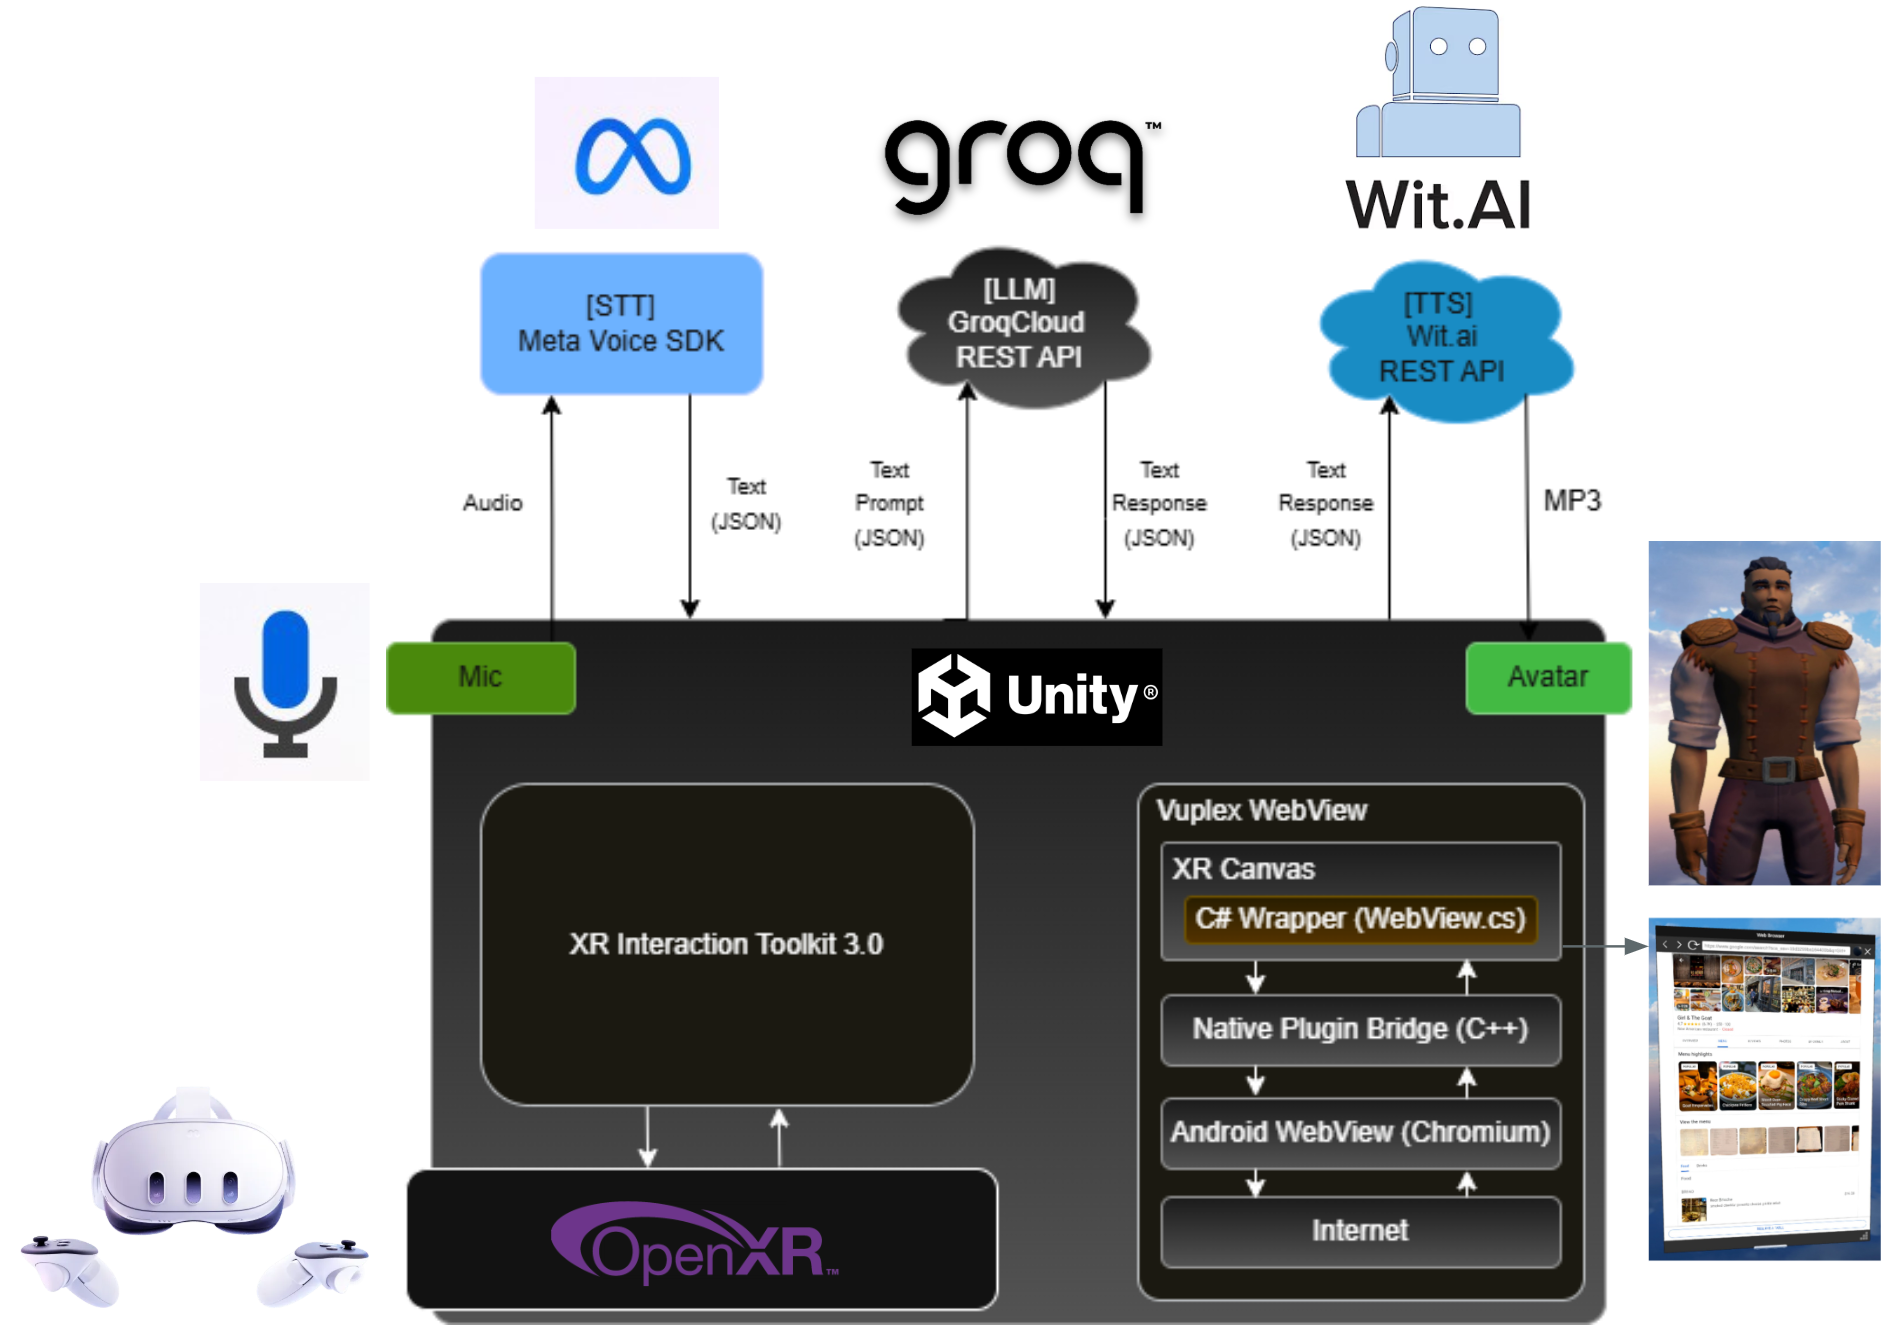
\includegraphics[width=0.9\textwidth]{fig/ss_mindpool/MP_System_Architecture_2.png}
    \caption{System Architecture Overview}
    \label{fig:System_Architecture}
    \end{figure}

\begin{itemize}
    \item \textbf{Unity 2022.3.5f1}: Unity was chosen as the primary development environment due to its rich ecosystem of XR tools, support for multiple platforms, and an extensive asset store. It also provides a user-friendly interface and well-maintained documentation, making it ideal for iterative development and testing of XR applications like MindPool especially with their Mixed Reality and Virtual Reality templates.
    
    \item \textbf{XR Interaction Toolkit (XRI) 3.0}: This toolkit was used for handling common XR interactions such as object grabbing, teleportation, and UI manipulation. XRI 3.0 simplifies multi-input support (controllers and hand tracking) and is tightly integrated with Unity's XR stack.
    
    \item \textbf{OpenXR}: OpenXR was selected for its cross-platform compatibility, allowing future deployment of MindPool to other headsets beyond the Meta ecosystem (e.g., HTC Vive, Valve Index, Varjo, HoloLens). This ensures long-term flexibility and scalability of the application.

    \item \textbf{Meta Voice SDK}: Integrated for enabling voice interactions, the Meta Voice SDK handles speech-to-text processing using \texttt{wit.ai}, enabling users to interact naturally with the AI Avatar and input content hands-free. This significantly improves accessibility and immersive experience.
    
    \item \textbf{Grok LLM}: The AI features such as the AI Note and AI Avatar rely on Grok LLM to process user inputs and generate meaningful natural language responses.

    \item \textbf{Vuplex 3D WebView (Modified)}: A customized version of the Vuplex browser asset was used to support multiple floating browser windows in XR. These windows replicate traditional browser UI elements (navigation buttons, URL bar) and can be manipulated from any distance.

    % \item \textbf{Unity Asset Store Skyboxes}: Free, high-quality skyboxes were used for immersive background environments. These include scenes like sunrise, sunset, space, and more, dynamically switchable by the user.

    \item \textbf{AcqKnowledge 5.0}: Used post-study to analyze physiological signals (e.g., heart rate, EDA, temperature) recorded by the Biopac Research Ring during user sessions.

    
\end{itemize}

\subsection{Hardware}

\begin{itemize}
    \item \textbf{Meta Quest 3}: MindPool was primarily developed and tested on Meta Quest 3, chosen for its support of mixed reality passthrough, improved resolution and performance, and growing user base. The headset provides all necessary features including hand tracking, voice input, and controller support.
    
    \item \textbf{Meta Quest 2, Quest 3s, and Quest Pro}: Additional testing was conducted on these Meta devices to ensure consistent user experience. MindPool’s input systems support both controller-based and hand-tracking modes using Meta’s APIs.

    \item \textbf{Biopac Research Ring (External Use)}: While not integrated directly into the application, the Biopac Research Ring was used in parallel during user studies to collect physiological data such as heart rate, EDA, and temperature. Some of these data was analyzed externally for evaluating stress and cognitive load.
\end{itemize}


% \subsection{Hardware and Platform Support}

% MindPool was developed and tested primarily on \textbf{Meta Quest 2}, \textbf{Meta Quest 3}, \textbf{Meta Quest 3s}, and \textbf{Meta Quest Pro} headsets. These devices support both controller-based and \textbf{hand-tracking input}, the latter of which was fully supported in MindPool using Meta’s Hand Tracking APIs.

% The application also leverages Meta’s system keyboard, which offers an improved UI, high-quality \textbf{haptic feedback}, and reliable \textbf{voice input}—significantly improving the text entry experience compared to custom-built XR keyboards.

% Compatibility was ensured using the OpenXR standard, which theoretically supports a broader range of XR devices including HTC Vive, Valve Index, Varjo, and HoloLens. However, actual testing and optimization were focused on Meta Quest headsets, which formed the target hardware for the study. No performance benchmarking under varying loads was conducted, although the final application build maintained a lean size of approximately \textbf{500 MB}—half the size of Noda’s 1 GB—resulting in lower storage overhead and faster load times.




\section{Core Features}



MindPool introduces a variety of enhancements compared to existing XR applications like Noda, focusing on usability, accessibility, and cognitive support. Table~\ref{tab:noda-comparison} summarizes key differences.

\begin{table}[h]
    \centering
    \caption{Feature comparison between MindPool and Noda}
    \label{tab:noda-comparison}
    \begin{tabular}{|p{3cm}|p{7cm}|p{5cm}|}
        \hline
        \textbf{Feature} & \textbf{MindPool} & \textbf{Noda} \\
        \hline
        Browser Instances & Multiple resizable browsers & Single browser instance \\
        \hline
        Note Structure & Title and content fields, movable, resizeable from any distance & Basic text nodes, proximity-limited manipulation \\
        \hline
        Link Creation & Connect notes, browsers from any distance & Requires physical proximity \\
        \hline
        Menu System & Minimalist head-following UI & Stationary menu \\
        \hline
        AI Support & AI Note + AI Avatar with content-aware voice responses (Grok LLM + TTS/STS) & Generate basic mind map with a prompt (Freemium) \\
        \hline
        Environment Options & 10 HD environments & Four free environments; additional options paywalled \\
        \hline
        Music Support & Stream any online music via additional browser (e.g., YouTube) & Built-in music, limited selection, most locked behind paywall \\
        \hline
        Keyboard Integration & Meta Quest System Keyboard & Custom VR keyboard with usability issues \\
        \hline
        Tutorial System & In-app video player with full-feature walkthrough & Step-by-step tutorial with restricted navigation \\
        \hline
        Controller Mapping & Visual floating labels for all buttons with clearly defined actions & Limited visual guidance \\
        \hline
        Accessibility & Voice input via AI Avatar benefits users with motor limitations & No AI Note or Avatar. Spotty Speech-to-Text \\
        \hline
        Size & 500 MB & 1 GB \\
        \hline
    \end{tabular}
\end{table}


% \begin{table}[h]
%     \centering
%     \caption{Feature comparison between MindPool and Noda}
%     \label{tab:noda-comparison}
%     \begin{tabular}{|p{4cm}|p{5cm}|p{5cm}|}
%         \hline
%         \textbf{Feature} & \textbf{MindPool} & \textbf{Noda} \\
%         \hline
%         Browser Instances & Multiple windows, resizable & Single instance only \\
%         \hline
%         Note Structure & Title + content fields & Simple text node \\
%         \hline
%         Link Creation & From any distance & Requires proximity \\
%         \hline
%         Menu System & Head-following minimalist UI & Fixed radial menu \\
%         \hline
%         AI Support & Conversational avatar + AI node & None \\
%         \hline
%         Environment Options & Multiple high-fidelity skyboxes & Limited selection, some paywalled \\
%         \hline
%         Music Support & Stream from browser & Built-in, limited \\
%         \hline
%         Persistence & Fast JSON-based resume & Session resume supported \\
%         \hline
%         Hand Tracking & Supported & Supported \\
%         \hline
%     \end{tabular}
% \end{table}

\begin{itemize}

    \item Enhanced Note System: Notes in MindPool have a title field and a content field, resembling modern digital note-taking apps. Users can move notes around either by grabbing the header (similar to desktop UI) or using a VR handle, from any distance. This provides a more intuitive and flexible experience compared to Noda's proximity-limited interaction model.

    \begin{figure}[h!]
      \centering
      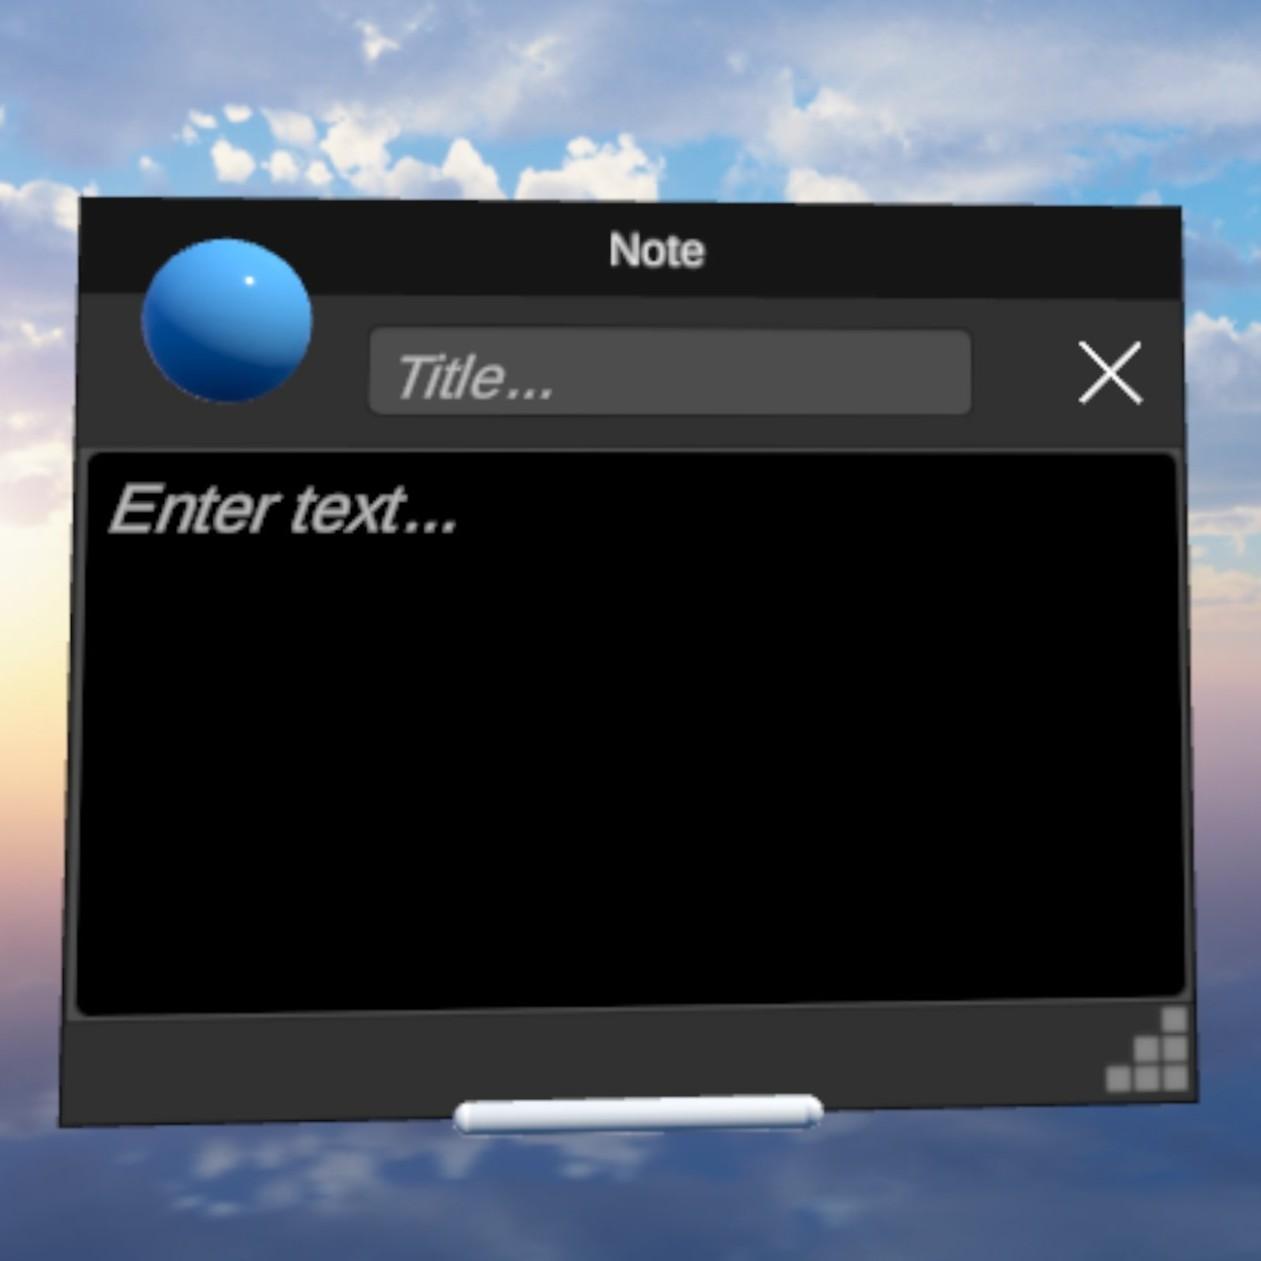
\includegraphics[width=0.48\textwidth]{fig/ss_mindpool/MP_Note.jpg} % Adjust width as needed
      \hfill % Adds horizontal space between the images
      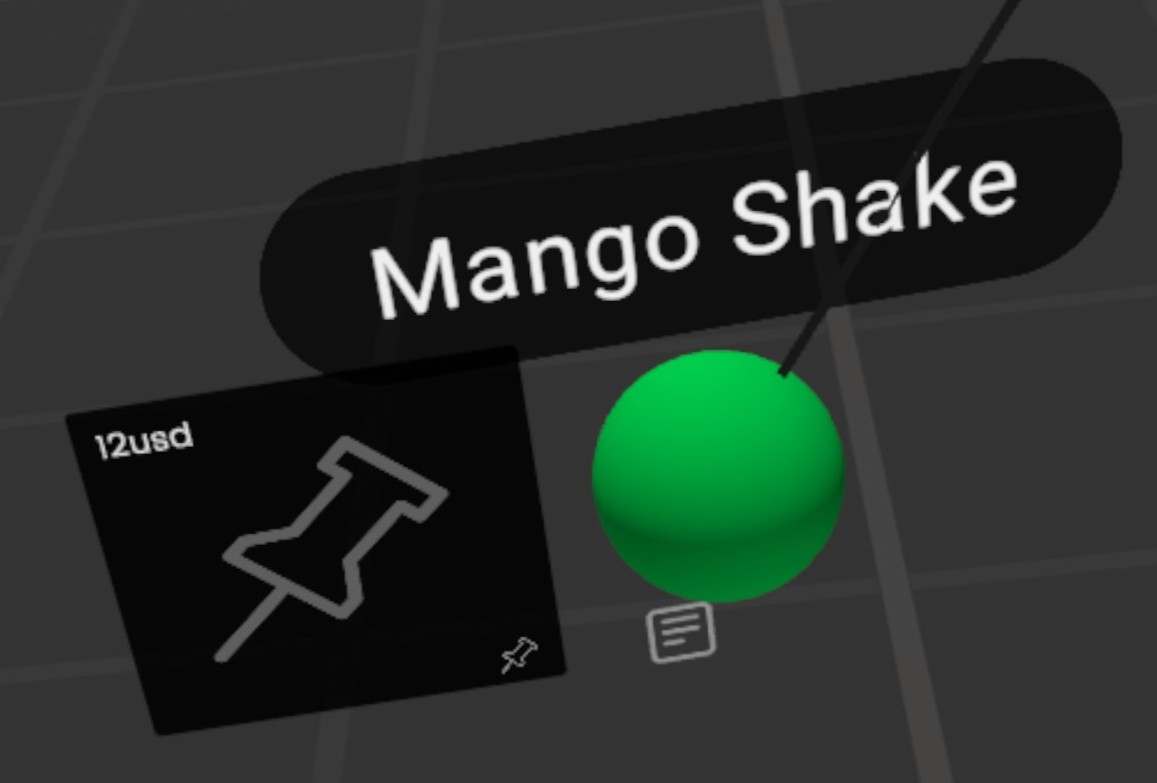
\includegraphics[width=0.48\textwidth]{fig/ss_noda/Noda_Note.jpg} % Adjust width as needed
      \caption{(Left) UI design of Mindpool's Note. (Right) UI design of Noda's Note.}
      \label{fig:sidebyside}
    \end{figure}


    \item Keyboard Integration: Instead of building a custom keyboard, MindPool leverages Meta Quest’s default system keyboard, which offers a highly polished and user-friendly typing experience, minimizing learning curve and input friction.

%     \begin{figure}[h]
%     \centering
%     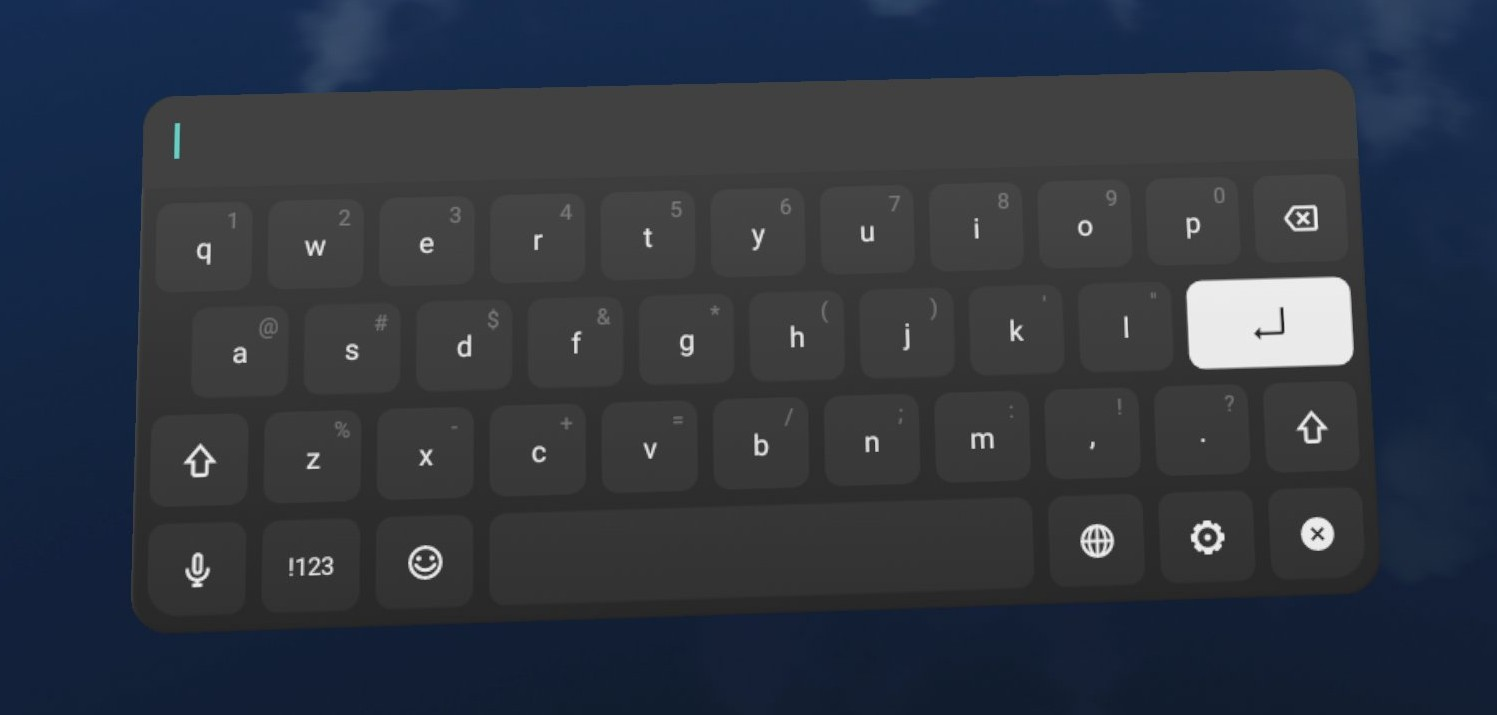
\includegraphics[width=0.75\textwidth]{fig/ss_mindpool/MP_Keyboard.jpg}
%     \caption{UI design of Meta's Keyboard used in MindPool.}
%     \label{fig:MP_Keyboard}
% \end{figure}

%  \begin{figure}[h]
%     \centering
%     \includegraphics[width=0.75\textwidth]{fig/ss_noda/Noda_KeyBoard.jpg}
%     \caption{UI design of Noda's Keyboard.}
%     \label{fig:Noda_Keyboard}
% \end{figure}

\begin{figure}[h!]
  \centering
  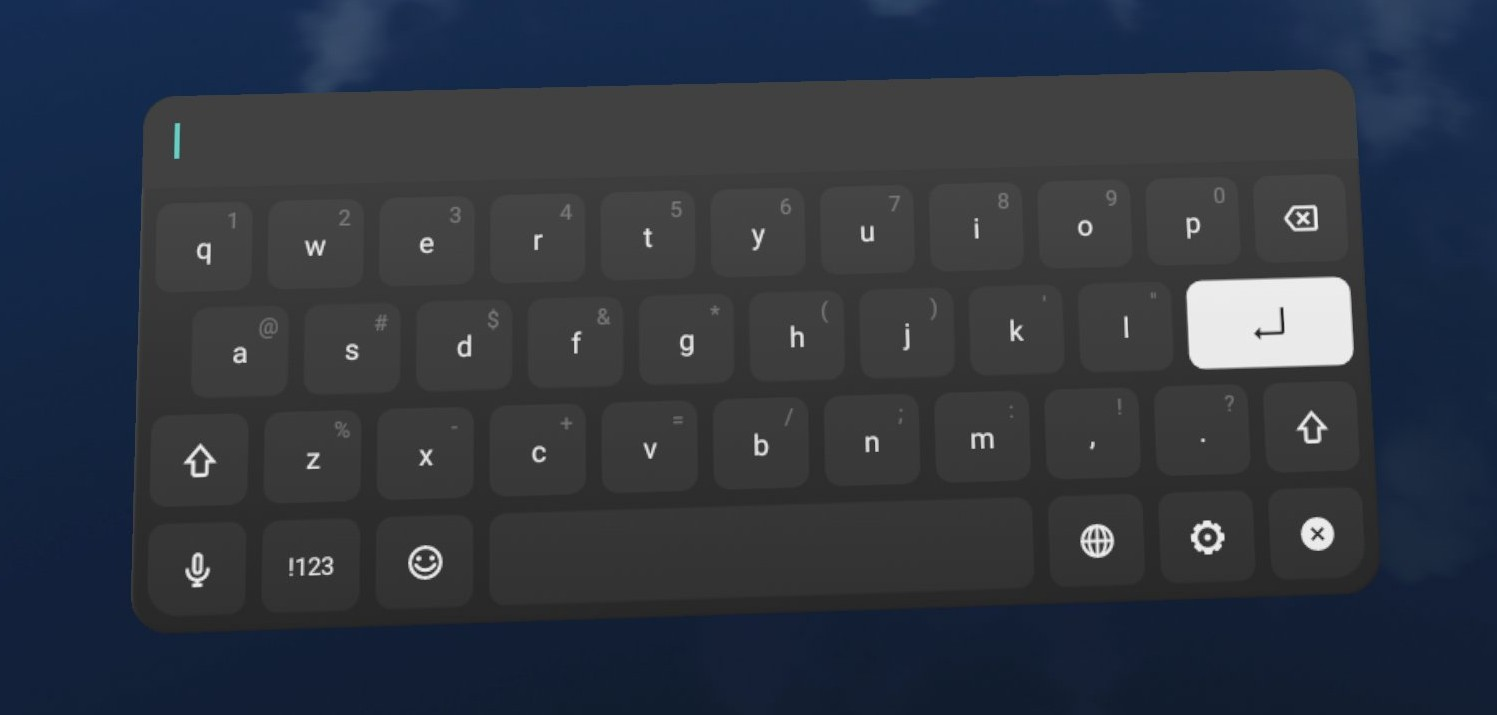
\includegraphics[width=0.48\textwidth]{fig/ss_mindpool/MP_Keyboard.jpg} % Adjust width as needed
  \hfill % Adds horizontal space between the images
  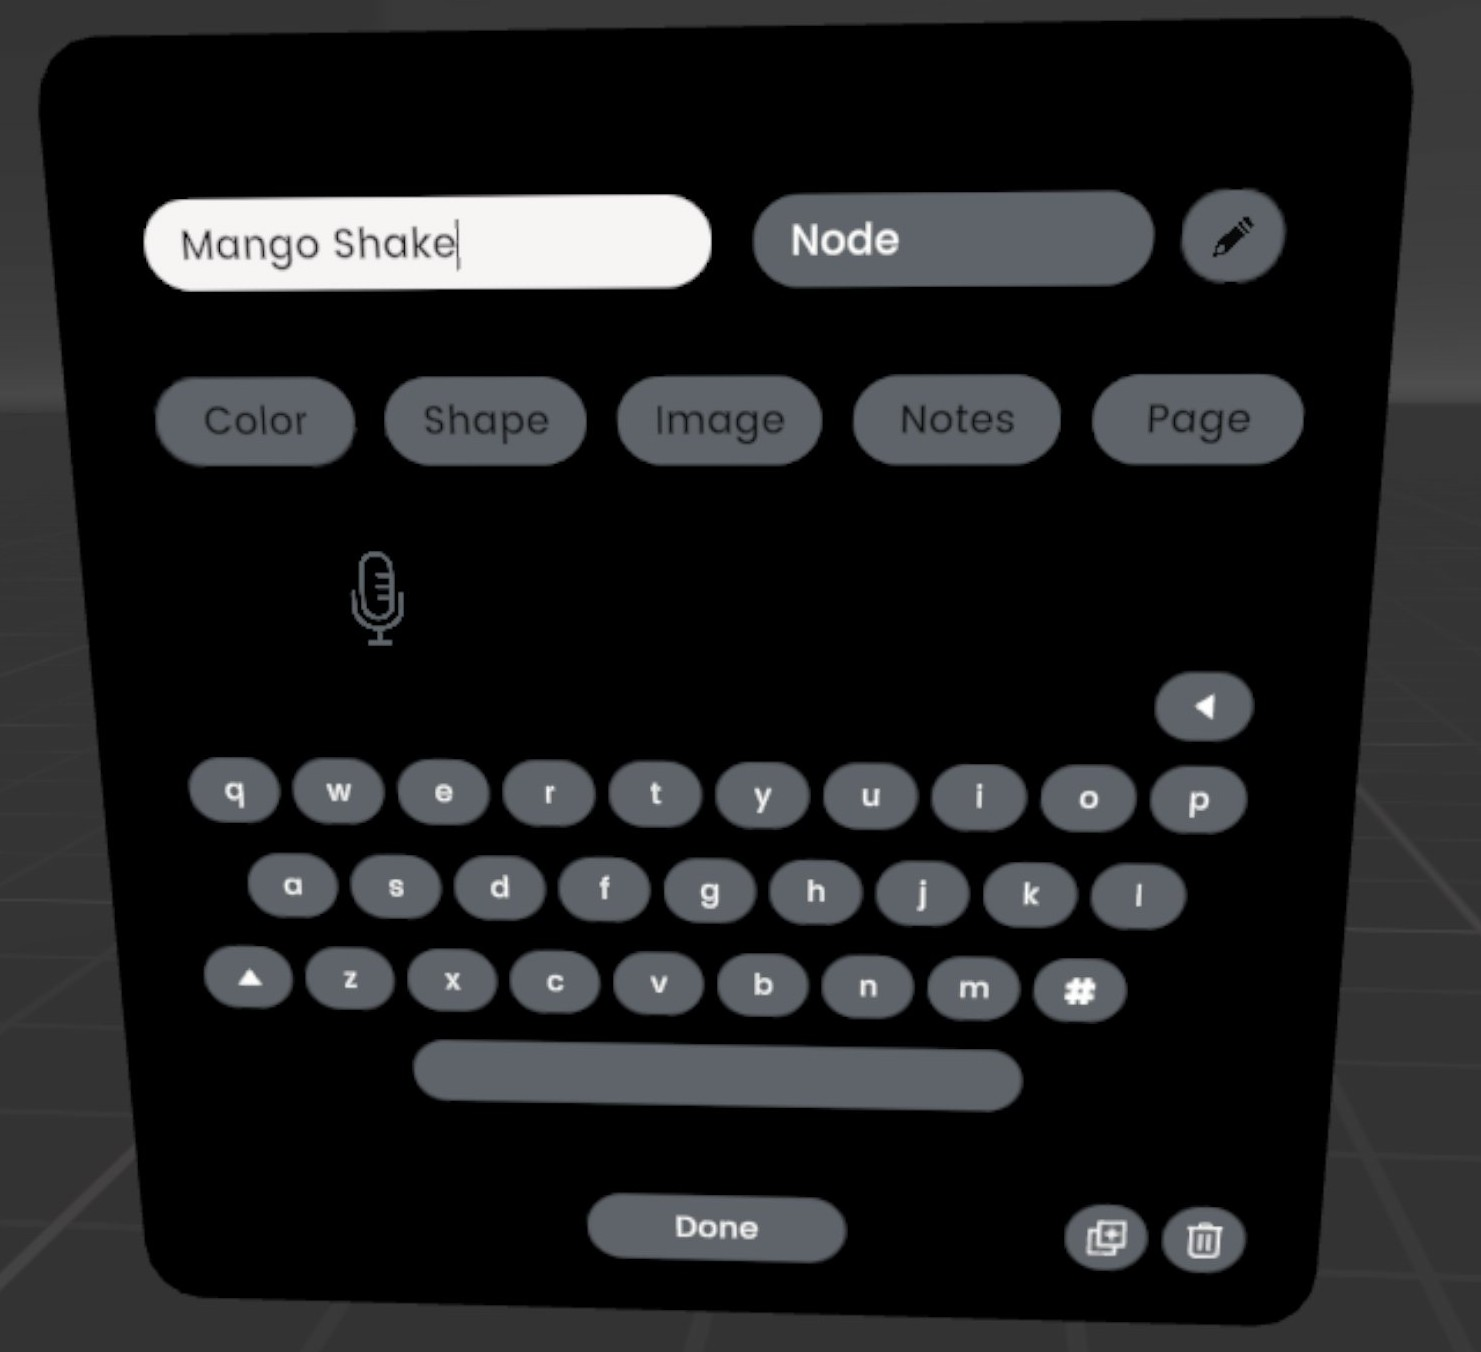
\includegraphics[width=0.48\textwidth]{fig/ss_noda/Noda_Keyboard2.jpg} % Adjust width as needed
  \caption{(Left) UI design of Meta's Keyboard used in MindPool. (Right) UI design of Noda's Keyboard for a node.}
  \label{fig:sidebyside}
\end{figure}
    
    \item Advanced Web Browsing: Using the Vuplex 3D WebView asset (which was extensively modified for XR use), MindPool allows users to spawn multiple browser windows simultaneously, resize them, and interact with them freely—an improvement over Noda, which only supports a single browser instance. The MindPool browser design mirrors conventional 2D browsers, with navigation buttons (back, forward, reload, close) and a visible URL bar placed at the top, enhancing familiarity and reducing cognitive overhead. Browsers and notes can be grabbed from any distance, unlike Noda which requires close proximity.

\begin{figure}[h!]
  \centering
  
\includegraphics[width=0.48\textwidth]{fig/ss_mindpool/MP_Browser.jpg} % Adjust width as needed
  \hfill % Adds horizontal space between the images
  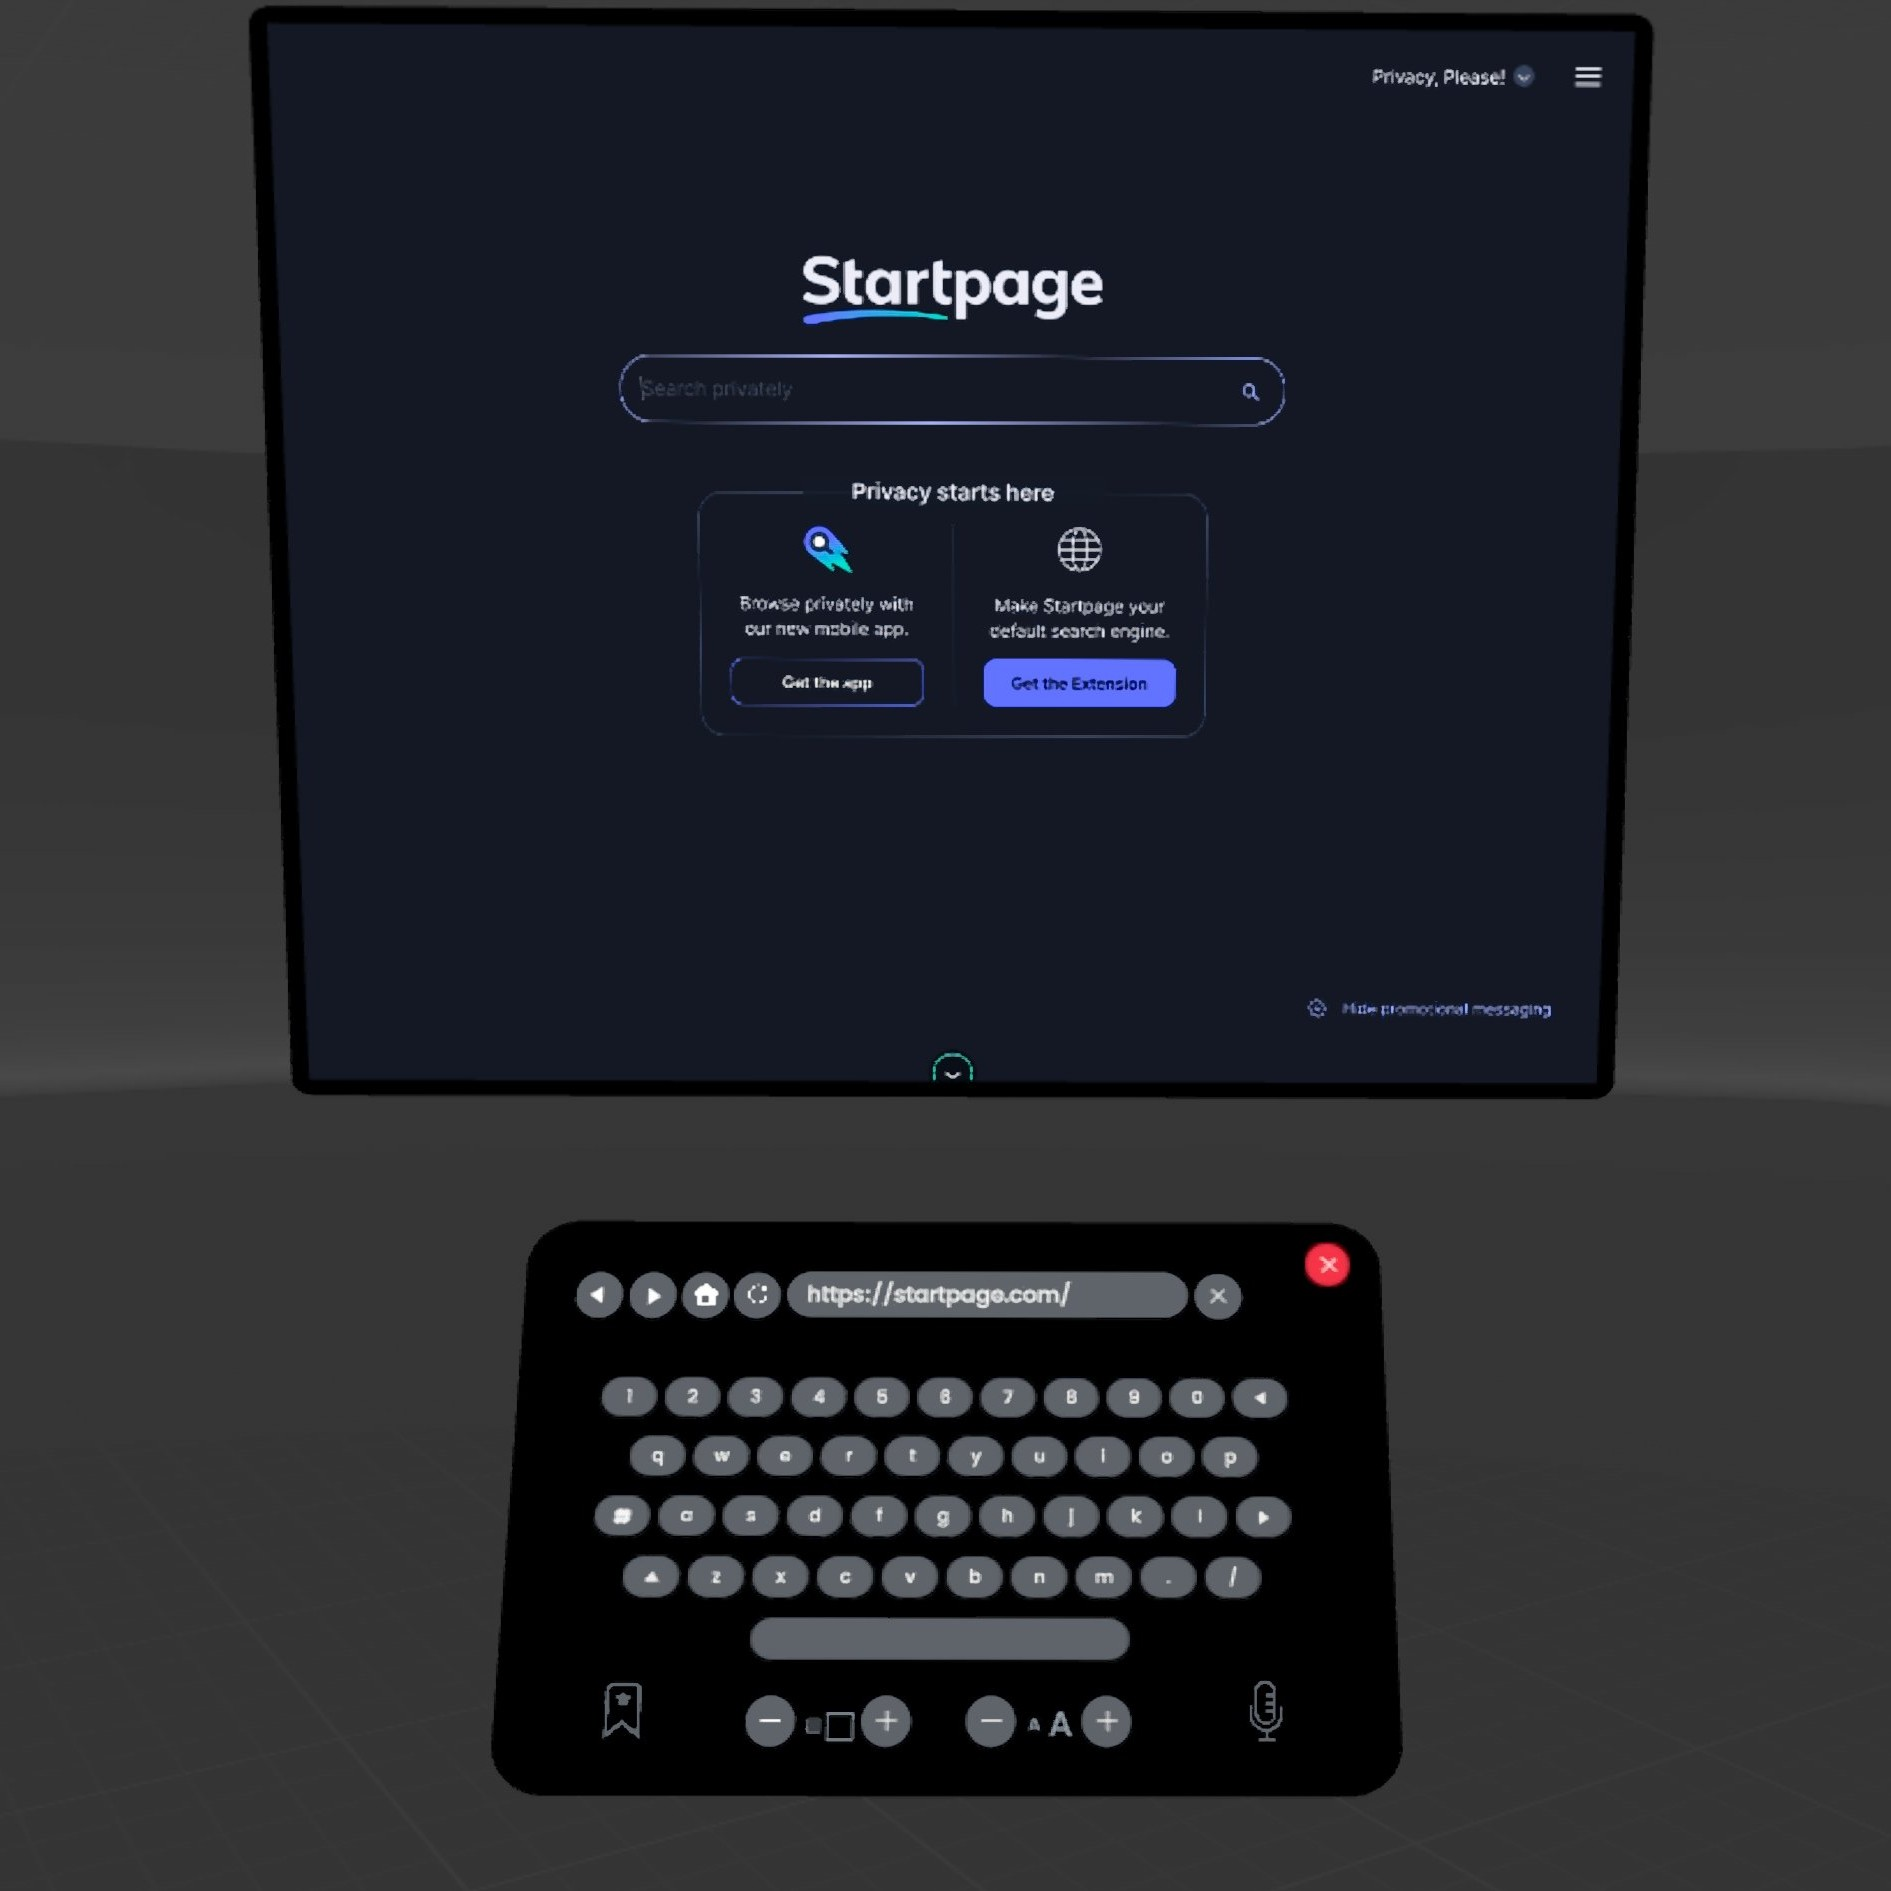
\includegraphics[width=0.48\textwidth]{fig/ss_noda/Noda_Browser.jpg} % Adjust width as needed
  \caption{(Left) UI design of Mindpool's browser. (Right) UI design of Noda's browser with an attached keyboard.}
  \label{fig:sidebyside}
\end{figure}
    
    
    
    \item Link Creation Flexibility: Creating connections between notes or browsers involves dragging from a node's sphere connector, similar to Noda. However, MindPool allows link creation from any distance, not requiring physical closeness to objects, which improves flow and usability.
    \item Streamlined User Interface and Menu System: MindPool’s menu is designed to be minimalist and follows the user’s head position for easy access. Unlike Noda’s menu system, it provides quick access to key functions without crowding the workspace.

% \begin{figure}[h!]
%   \centering
%   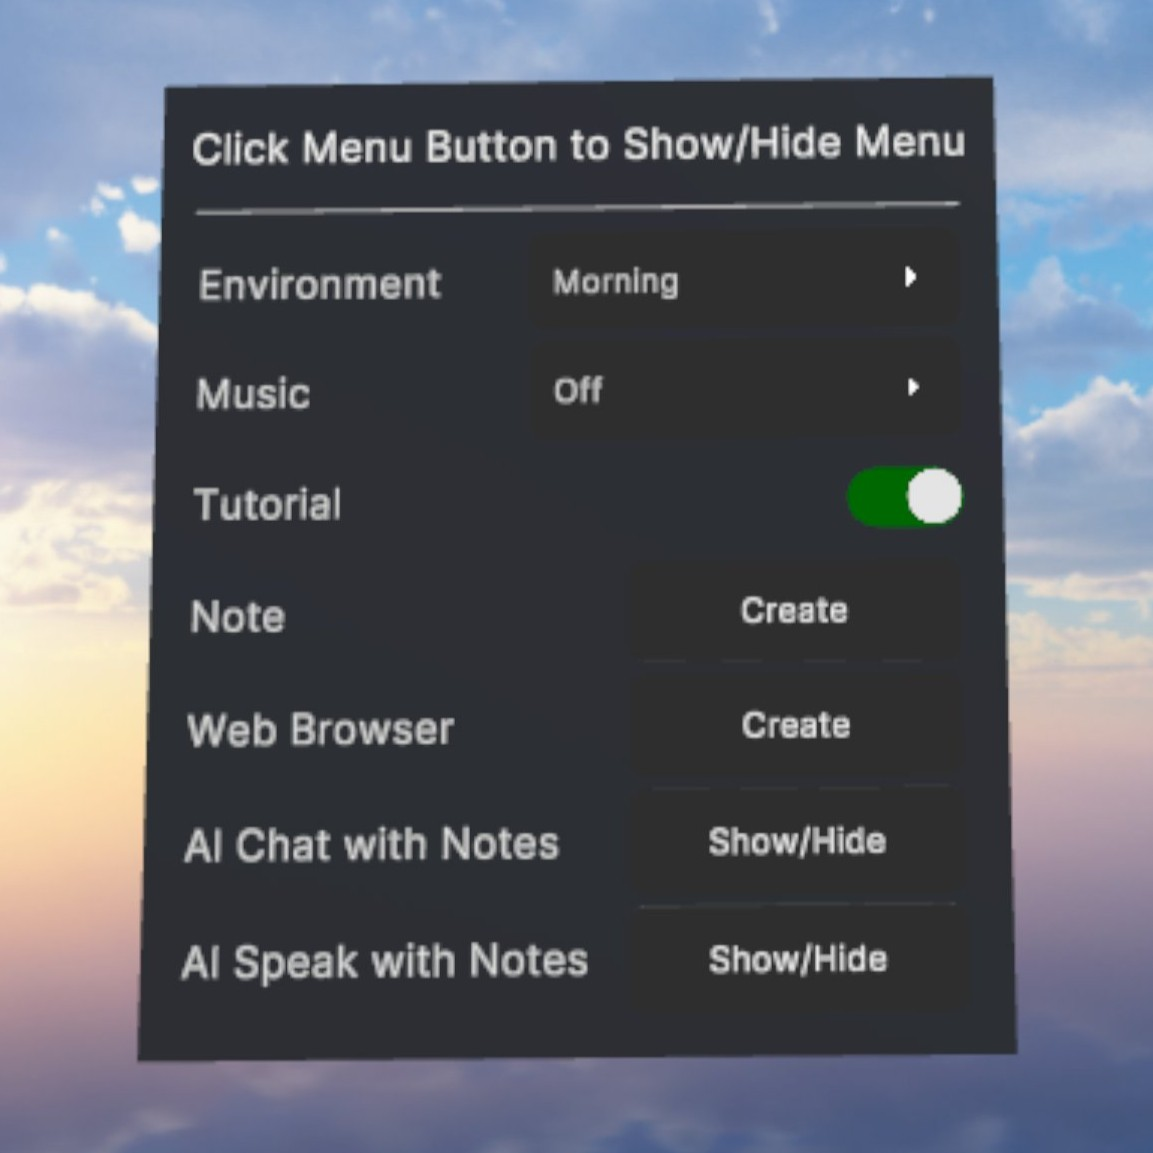
\includegraphics[width=0.48\textwidth]{fig/ss_mindpool/MP_Menu.jpg} % Adjust width as needed
%   \hfill % Adds horizontal space between the images
%   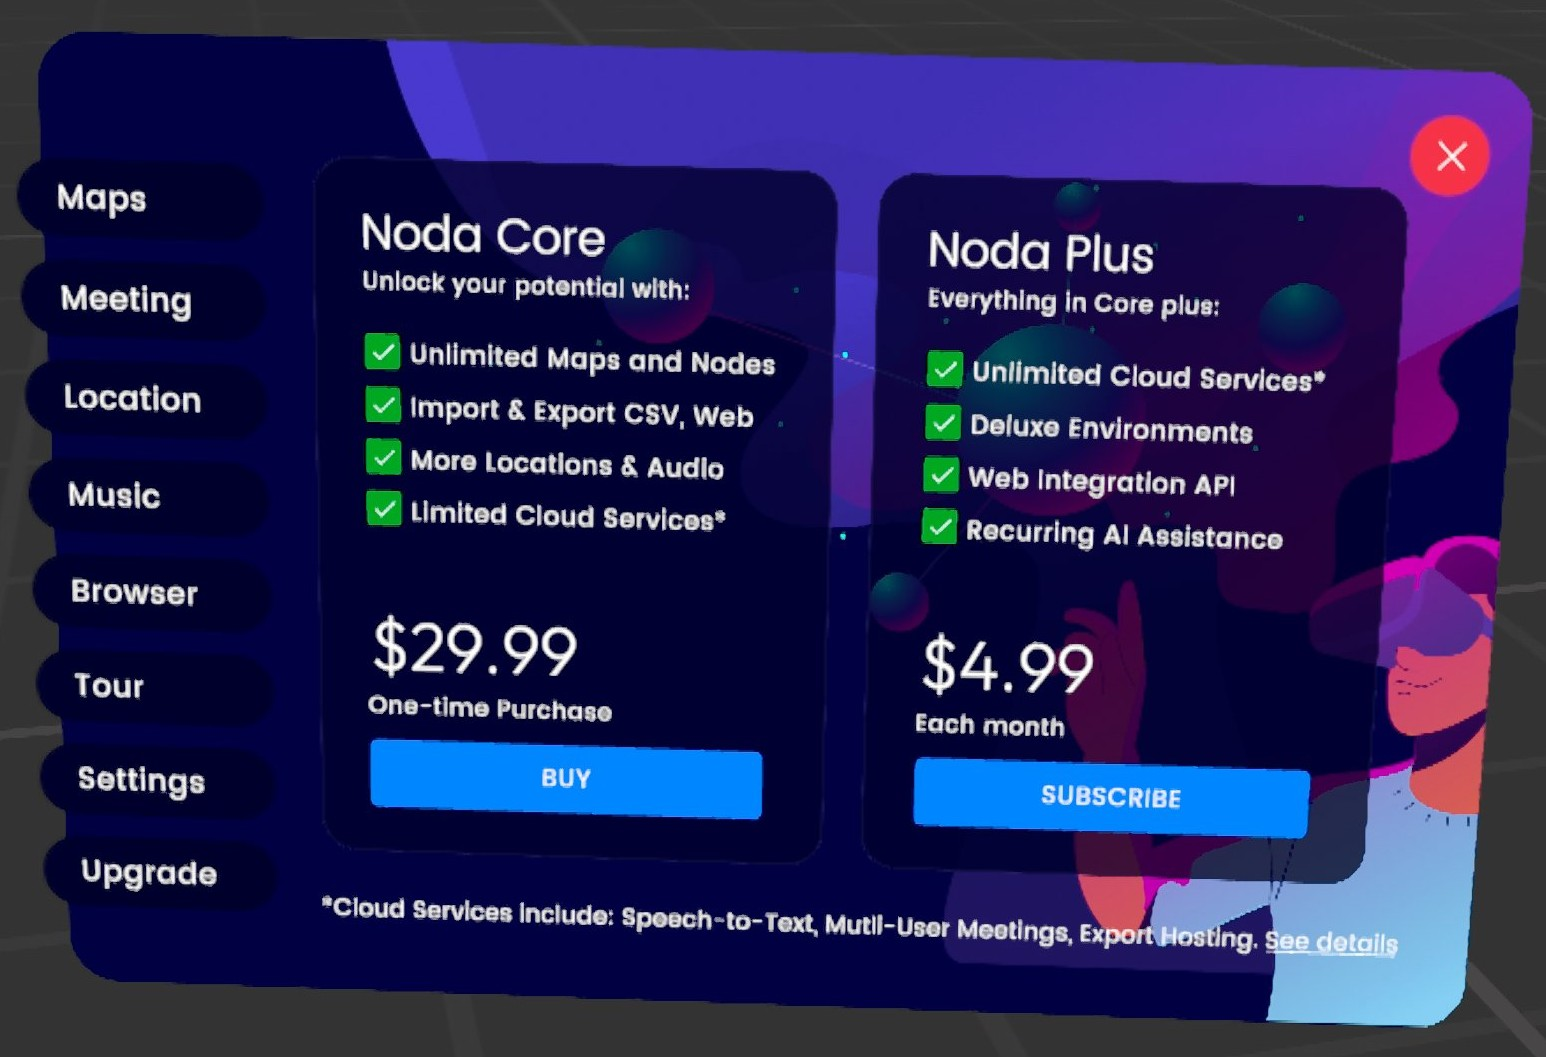
\includegraphics[width=0.48\textwidth]{fig/ss_noda/Noda_menu.jpg} % Adjust width as needed
%   \caption{(Left) UI design of MindPool's Menu. (Right) UI design of Noda's Menu.}
%   \label{fig:sidebyside}
% \end{figure}
    
    \item In-App Tutorial Video Player: A 7-minute tutorial video provides comprehensive onboarding for new users, covering all essential operations. This contrasts with Noda’s more restrictive follow-along tutorials that require sequential task completion and cover only partial functionality.

\begin{figure}[h!]
  \centering
  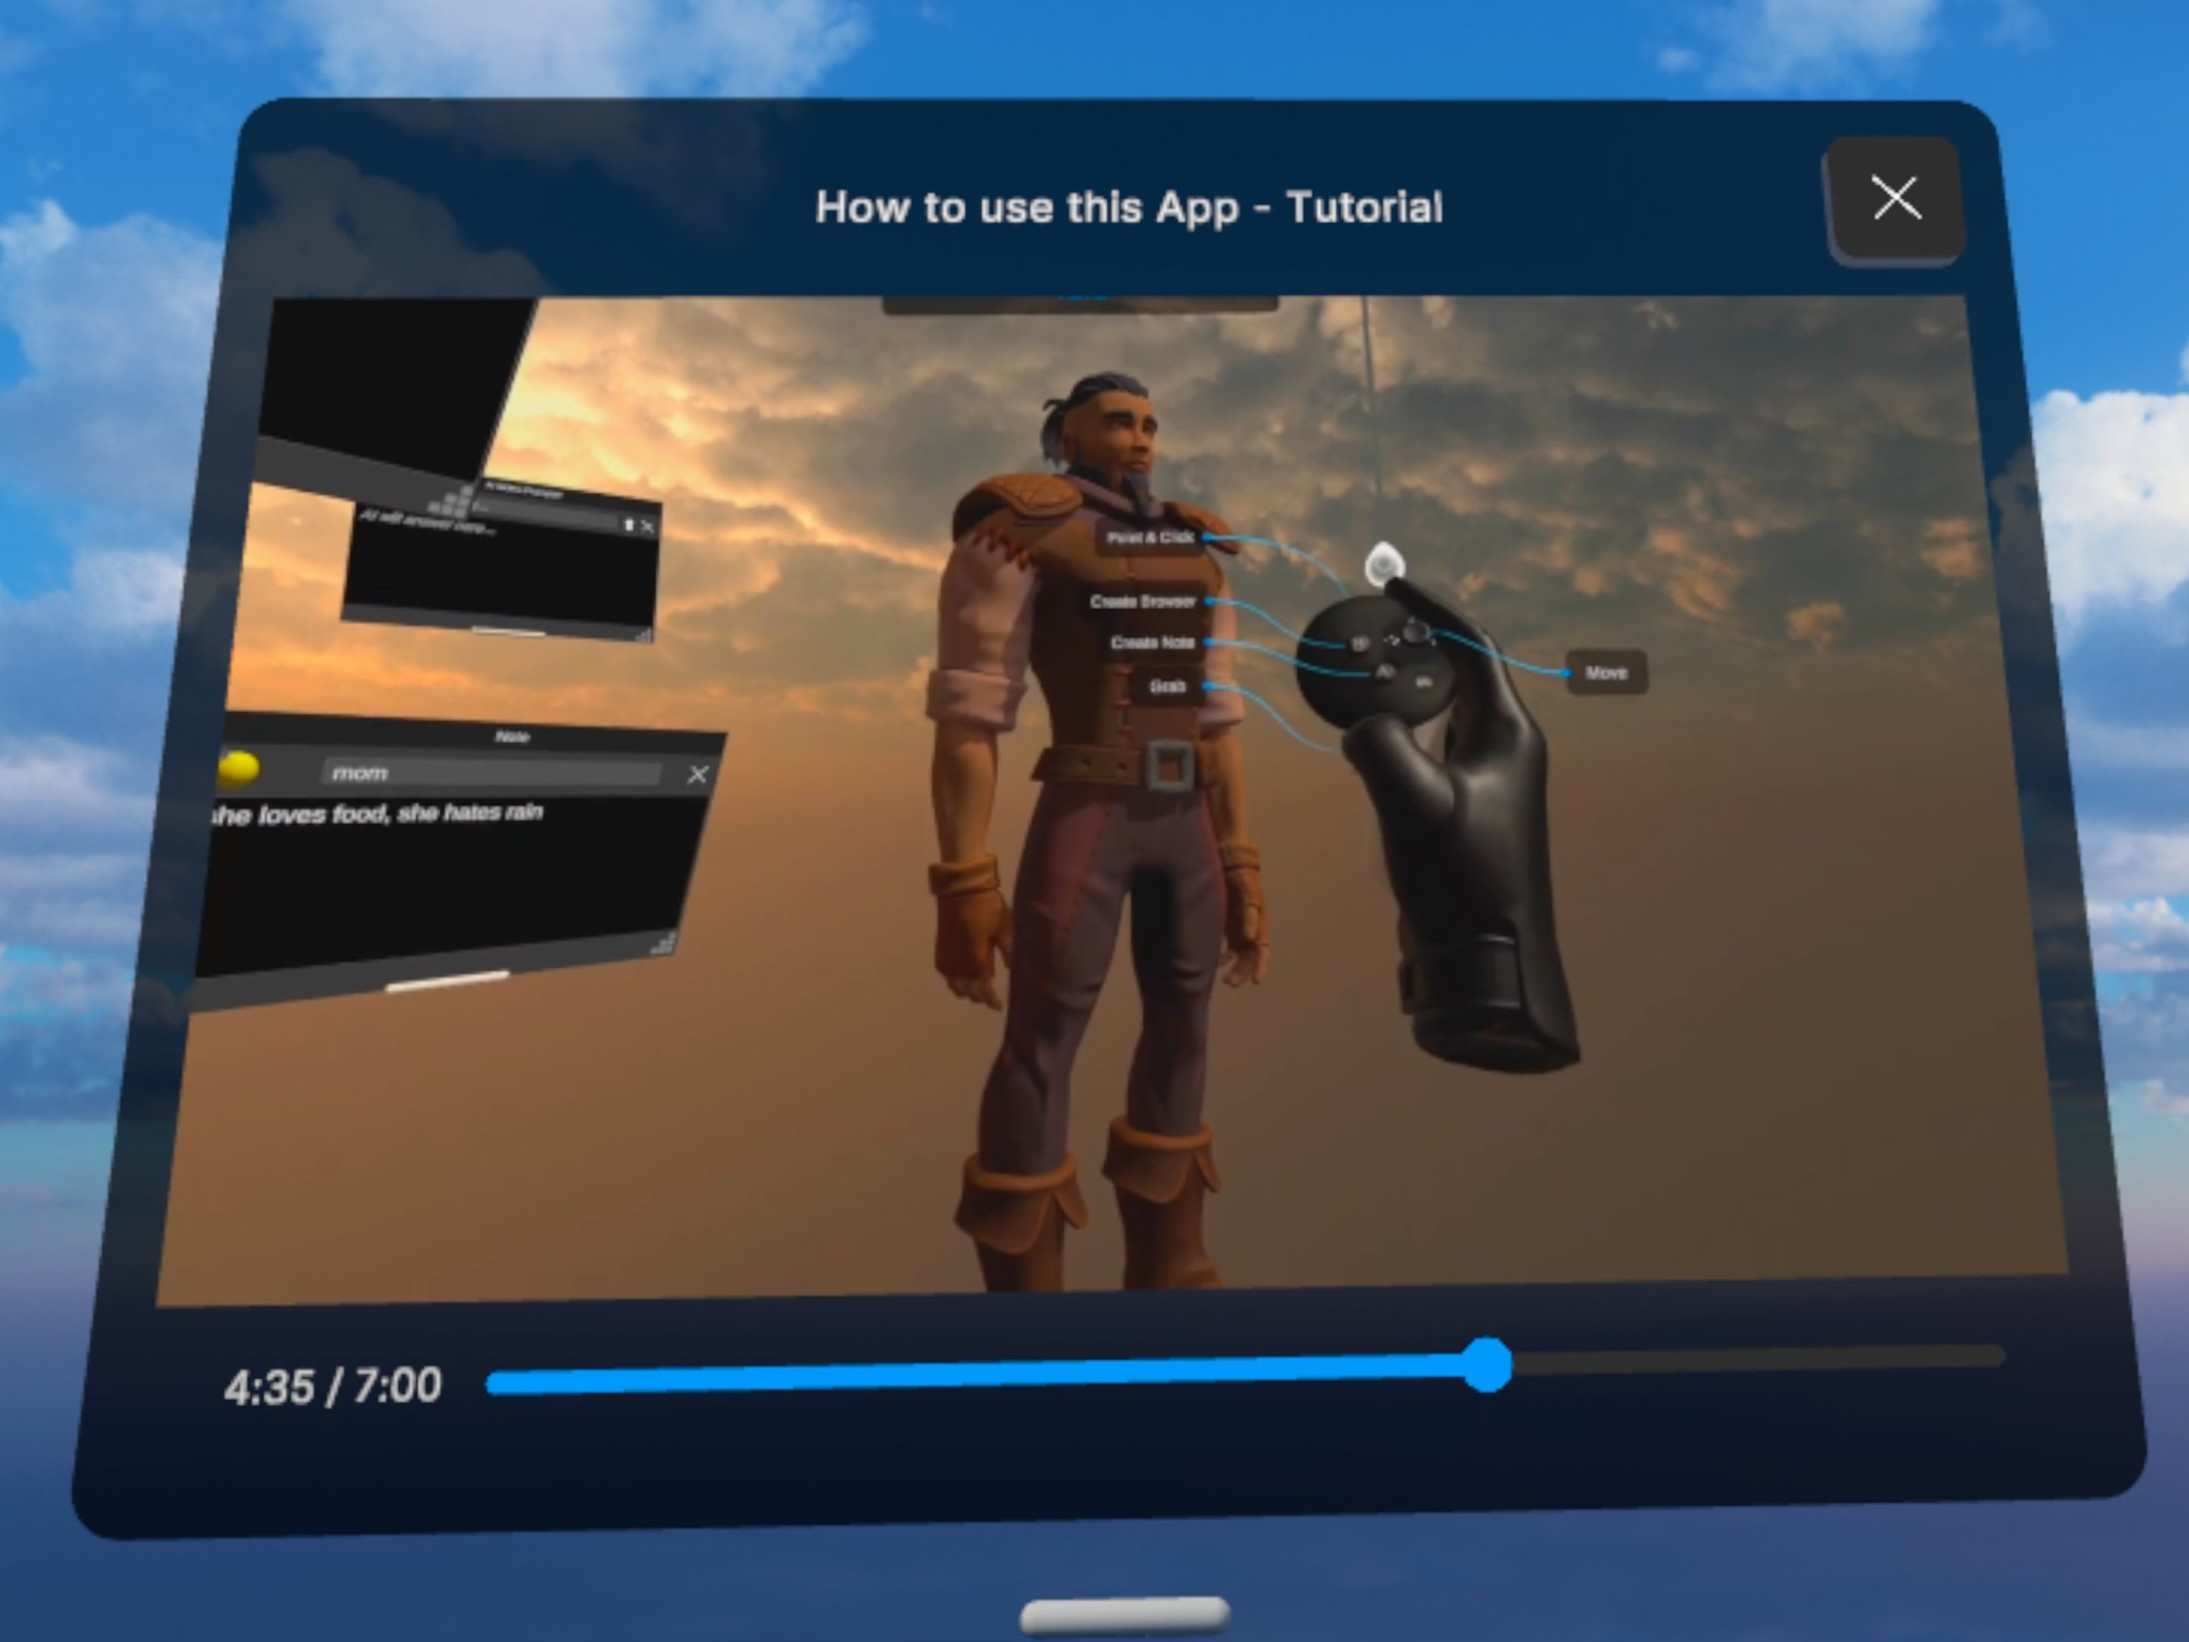
\includegraphics[width=0.48\textwidth]{fig/ss_mindpool/MP_Tutorial.jpg} % Adjust width as needed
  \hfill % Adds horizontal space between the images
  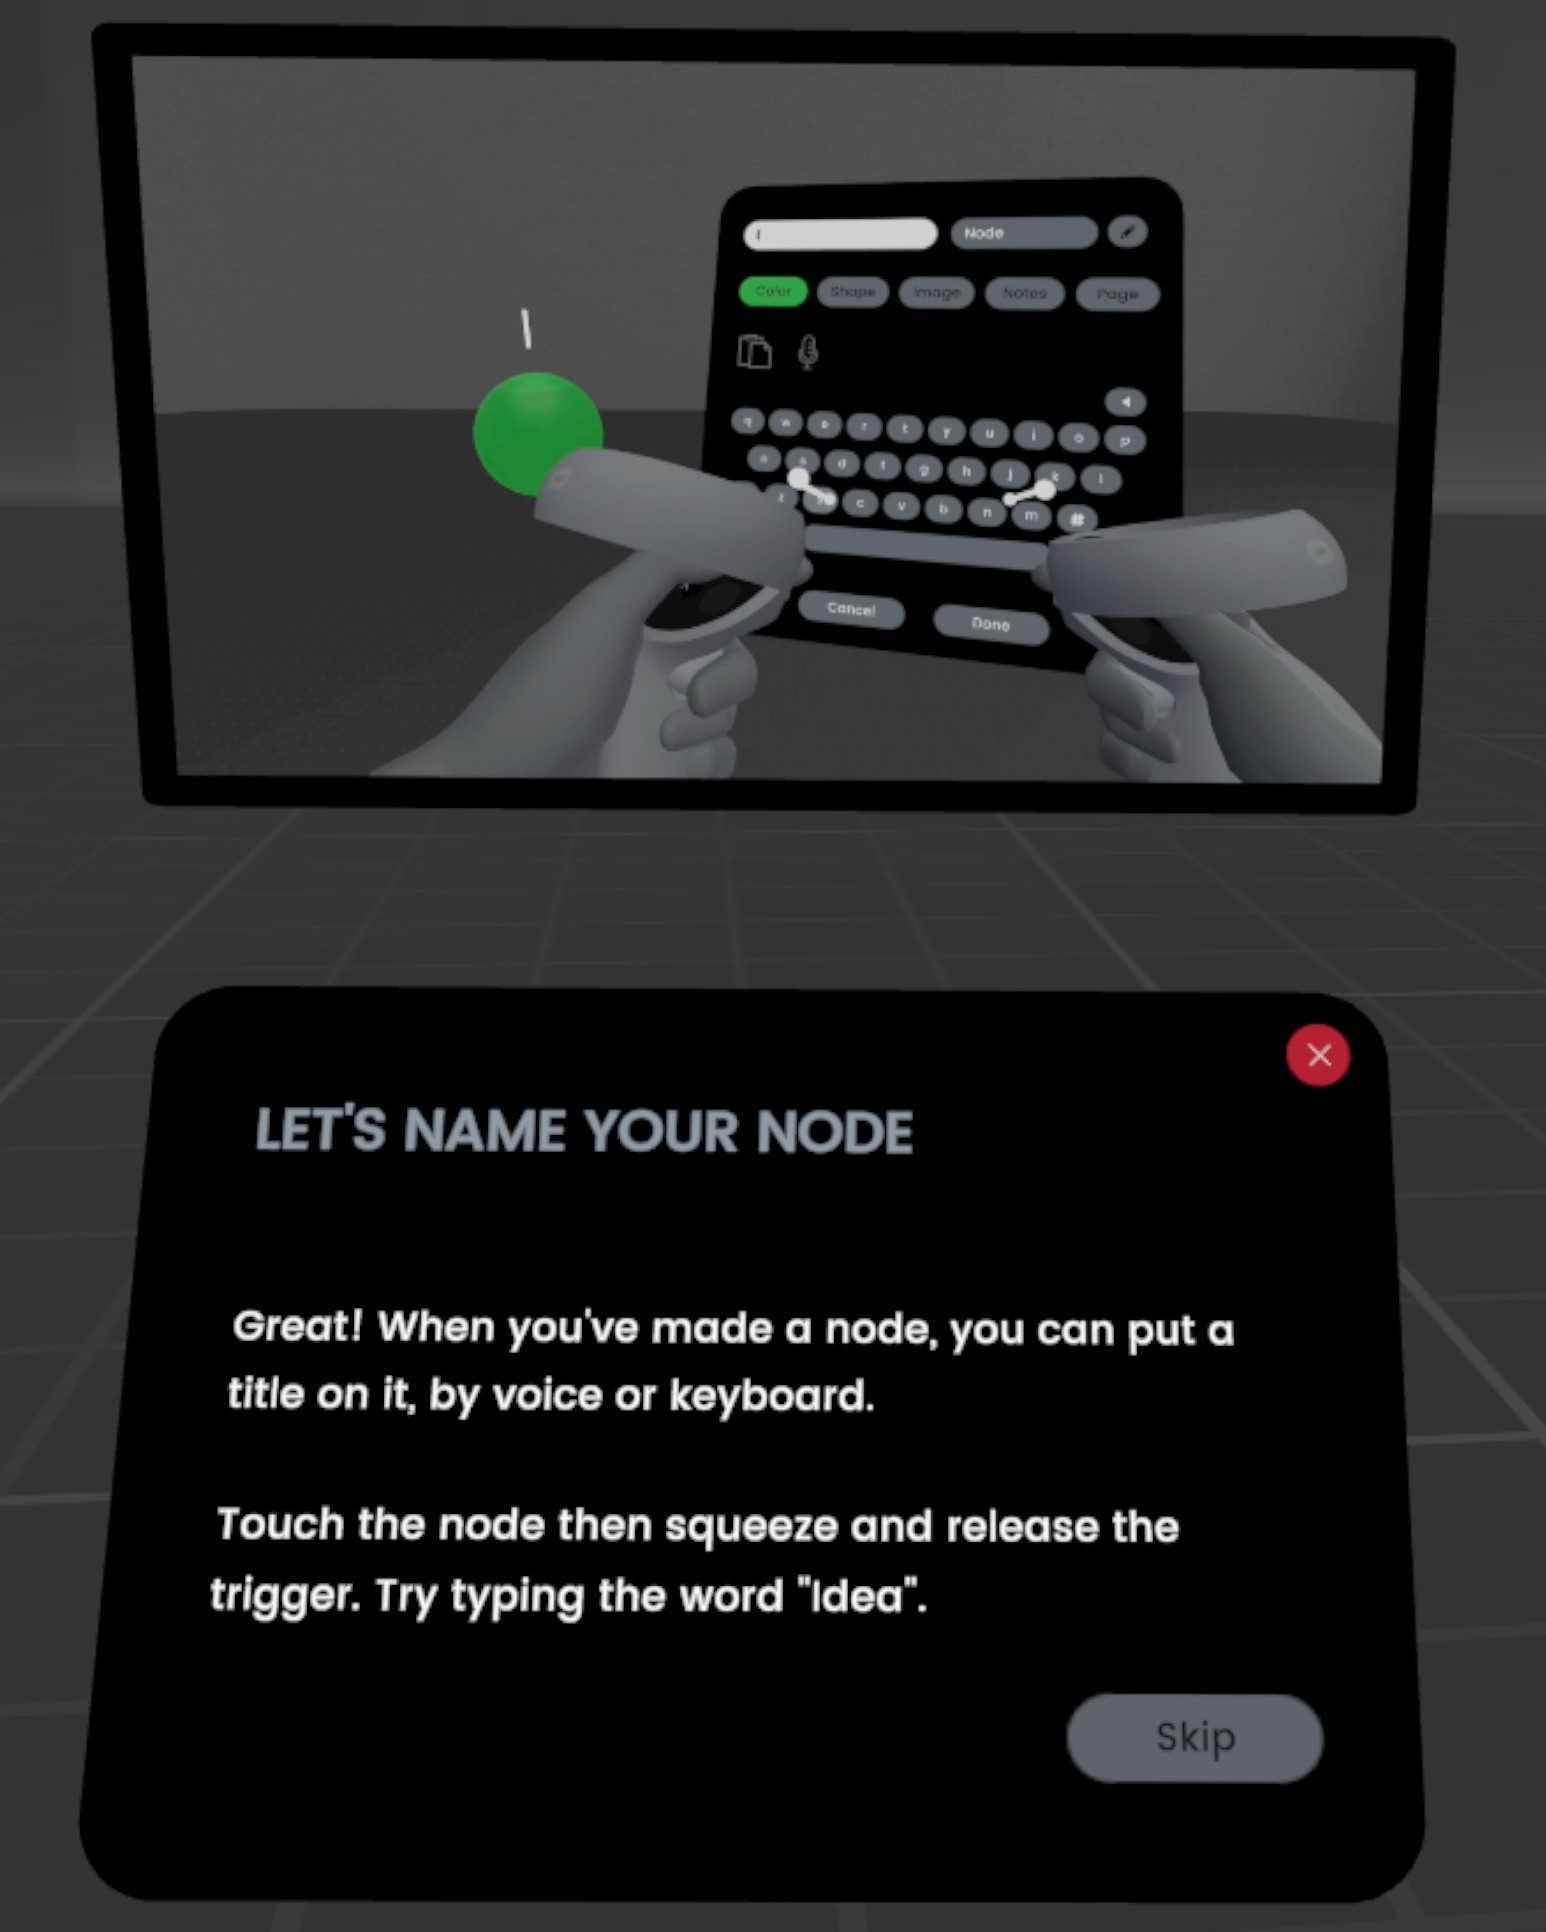
\includegraphics[width=0.48\textwidth]{fig/ss_noda/Noda_Tutorial.jpg} % Adjust width as needed
  \caption{(Left) Mindpool's Tutorial Video Player. (Right) Noda's Tutorial.}
  \label{fig:sidebyside}
\end{figure}
    
    \item Clear Control Mapping with Visual Cues: All controller buttons are mapped with visual floating labels that describe their functions:

    \begin{figure}[h!]
  \centering
  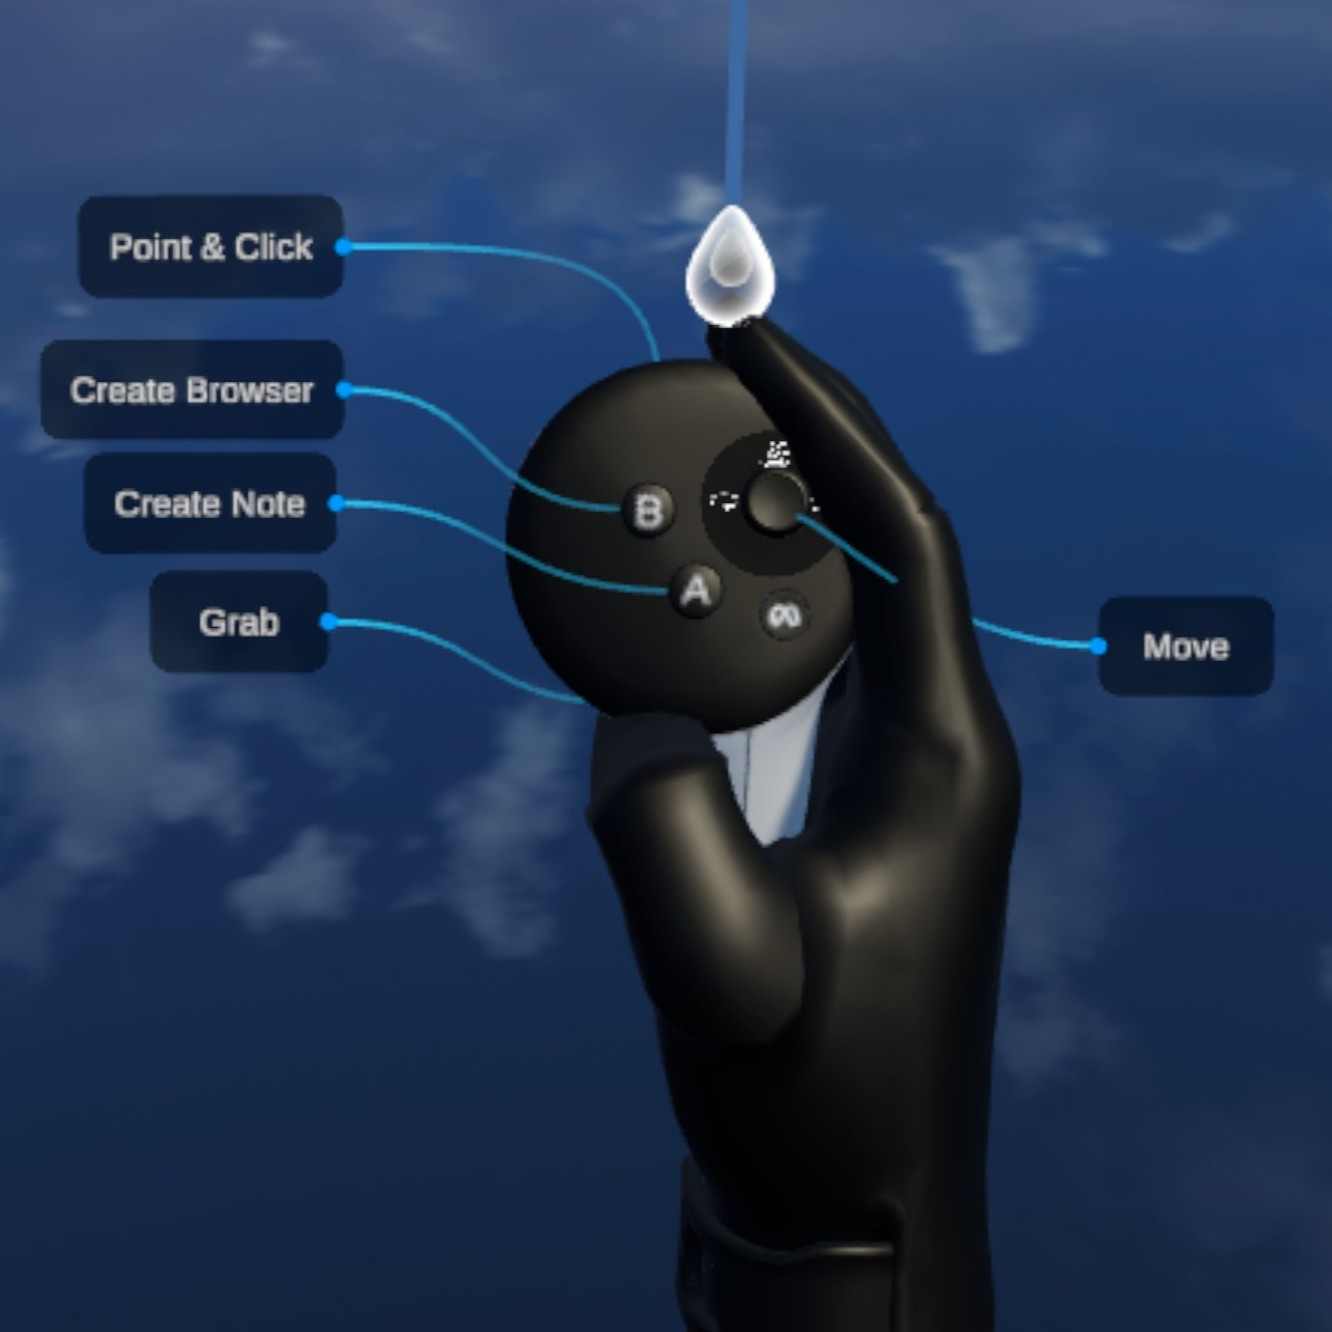
\includegraphics[width=0.48\textwidth]{fig/ss_mindpool/MP_Controller.jpg} % Adjust width as needed
  \hfill % Adds horizontal space between the images
  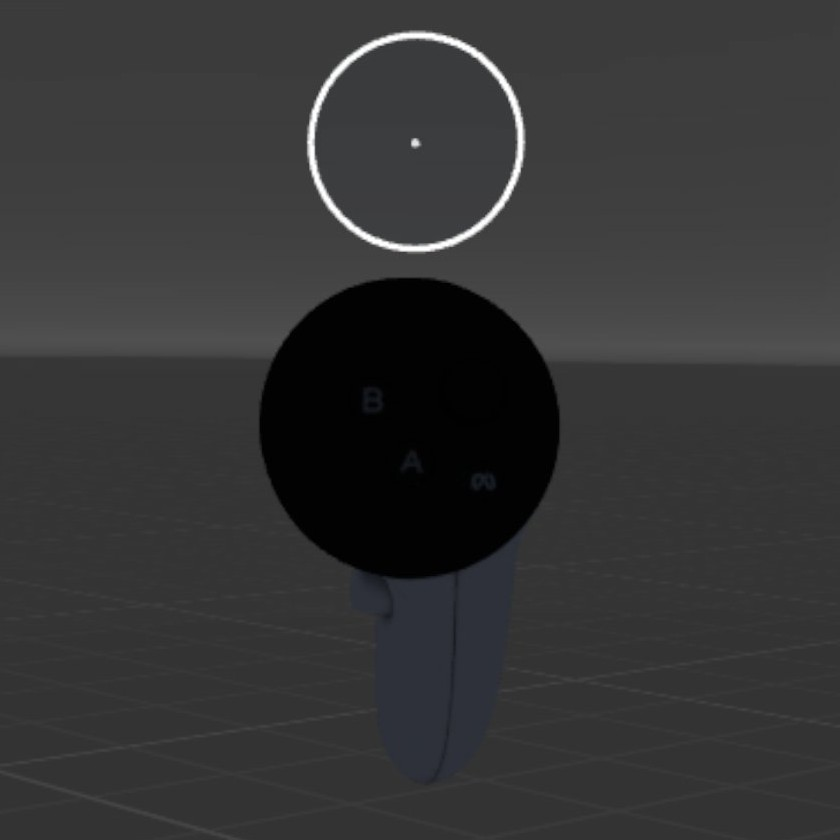
\includegraphics[width=0.48\textwidth]{fig/ss_noda/Noda_Controller.jpg} % Adjust width as needed
  \caption{(Left) MindPool's Controller. (Right) Noda's Controller.}
  \label{fig:sidebyside}
\end{figure}
    
    \begin{itemize}
        \item A button: Create new note
        \item B button: Spawn a new browser
        \item Hold Y button: Activate voice input for AI Avatar
        \item Right joystick: Move within the environment
        \item Grab button: Move or grab items
        \item Trigger button: Point and select
    \end{itemize}
    
    \item Environment and Background Options: MindPool offers a wider array of high-quality immersive environments, including sunrise, sunset, outer space, Milky Way, and passthrough mode, leveraging free, high-quality skyboxes from the Unity Asset Store. Noda also provides some complimentary immersive environments (four options). However, a more extensive selection is locked behind a paywall.
    
    \item Background Music Flexibility: Users can open a browser to stream any music of their choice (e.g., YouTube background audio) while mind mapping. Noda restricts background music to a limited built-in selection, with most options locked behind a paywall.
    
    \item AI Assistance and Conversational Avatar:
    
    \begin{itemize}
        \item AI Note: A specialized node that reads all notes and browser content to generate intelligent responses based on user prompts, using Grok LLM for query processing.
        \item AI Avatar: A humanoid conversational agent capable of understanding spoken questions (speech-to-text using Meta’s Voice SDK and wit.ai) and responding verbally (text-to-speech with animated hand gestures), offering a natural, personalized interaction experience. The inclusion of an AI Avatar also enhances accessibility by allowing users to interact with the system through voice commands rather than relying solely on physical controllers or text input, making the app more inclusive for individuals with motor impairments or limited typing proficiency.

    \begin{figure}[h]
    \centering
    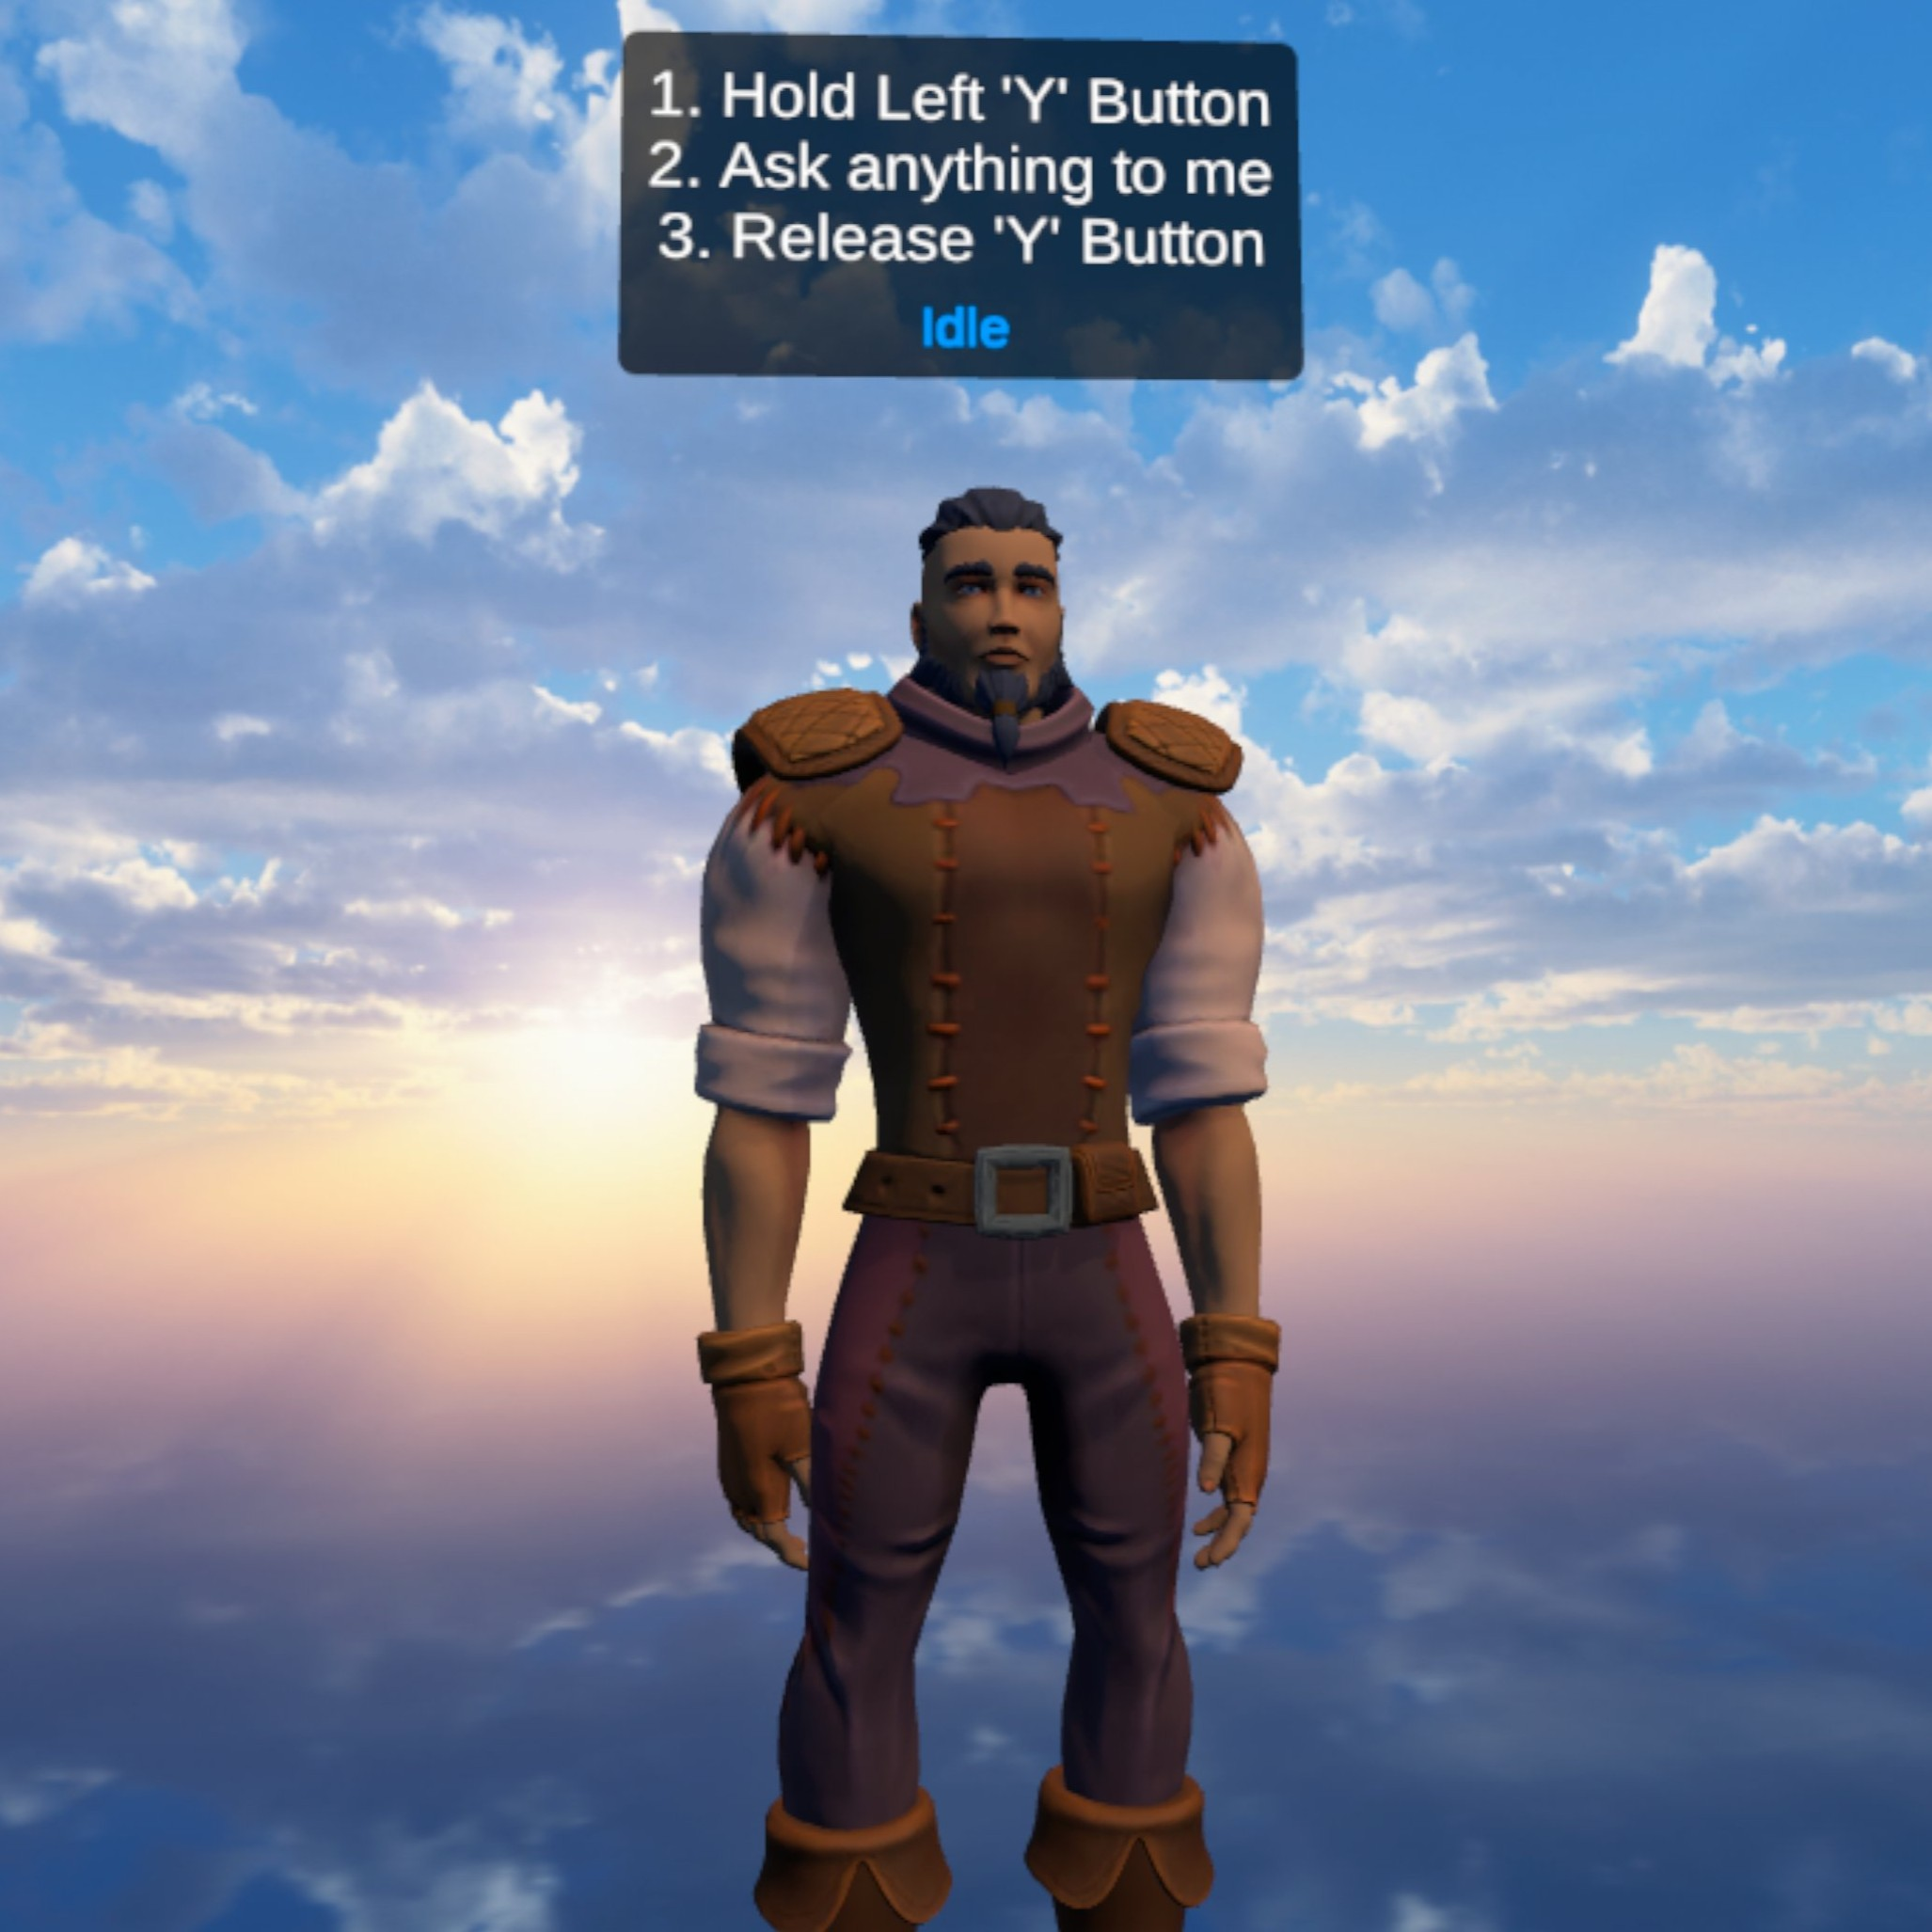
\includegraphics[width=0.9\textwidth]{fig/ss_mindpool/MP_AI_Avatar.jpg}
    \caption{AI Avatar used in MindPool.}
    \label{fig:MP_Keyboard}
    \end{figure}

Figure~\ref{fig:AI_Architecture} illustrates the architecture of the AI features integrated into the application. It presents a Unity-based conversational avatar pipeline that incorporates real-time speech-to-text (STT) using the Meta Voice SDK, natural language processing via the Groq Cloud LLM REST API, and text-to-speech (TTS) synthesis through the Wit.ai REST API.

\begin{figure}[h]
    \centering
    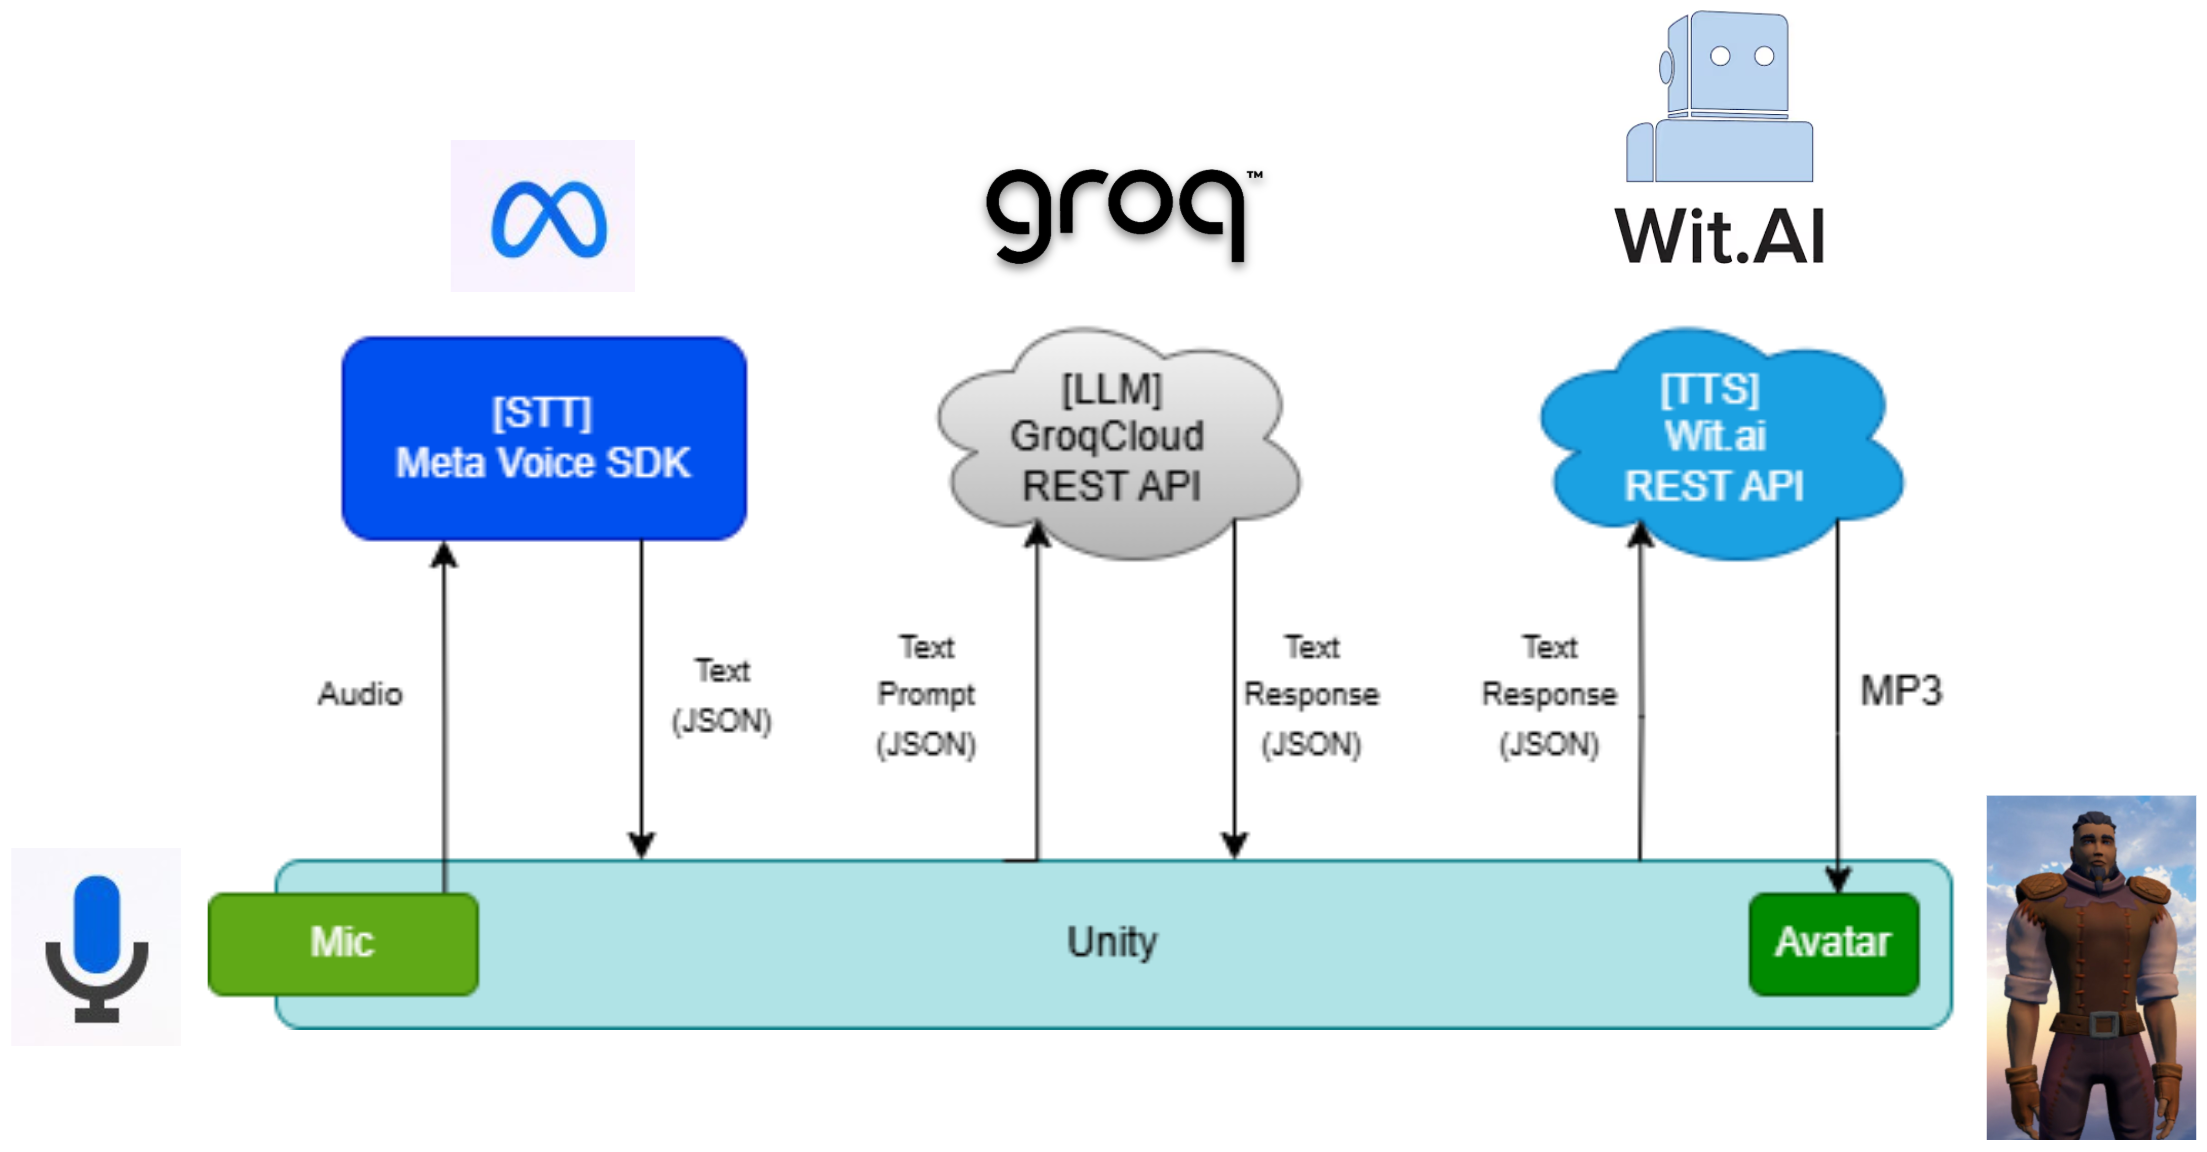
\includegraphics[width=1\textwidth]{fig/ss_mindpool/MP_AI_Architecture.png}
    \caption{End-to-End Voice Interaction Pipeline for XR AI Avatar}
    \label{fig:AI_Architecture}
    \end{figure}

    \end{itemize}
    
    \item Auto-Save and Resume Functionality: MindPool automatically saves all session data—including note contents, positions, orientations, and link connections—into a JSON file upon exit. Upon relaunch, the system reloads the previous workspace, allowing seamless session resumption. Although this feature is also present in Noda, MindPool implements it with lightweight file handling and quick load times.
    \item Hand Tracking Compatibility: MindPool supports both controller-based interaction and hand-tracking input using Meta’s Hand Tracking APIs, allowing users to drop their controllers and interact naturally via hand gestures, similar to Noda.
    \item Performance and Size Optimization: MindPool maintains a relatively small application size (approximately 500 MB) compared to Noda’s larger footprint (approximately 1 GB), ensuring faster downloads, smoother updates, and reduced storage impact on devices.
\end{itemize}

\section{Development Outcome Summary}

MindPool was developed with an emphasis on providing an improved intuitive, accessible, and cognitively supportive XR mind mapping experience. The key design principles guiding development included familiar UI, interaction flexibility, and support for multimodal input (voice, hand tracking, and controllers). These decisions were intended to reduce cognitive load, encourage user motivation, and improve overall usability.

Compared to existing XR mind mapping tools like Noda, MindPool introduces several unique contributions: an AI-enhanced note assistant (AI Note), a conversational humanoid avatar for natural voice interaction, a browser system that supports multiple simultaneous windows, a dual-field note interface, improved control mapping, a customizable environment system, and lightweight file-saving for seamless session resumption. Furthermore, the app includes a video tutorial player and controller visual cues for onboarding and guidance, and it leverages Meta’s system keyboard for better text input.

% The features implemented aligned with the research objectives of the study—namely, evaluating how immersive tools can improve motivation, usability, and cognitive workload in mind mapping tasks. While not all performance or hierarchy features were implemented, the innovations in interaction design and AI support make MindPool a valuable platform for studying user experience and physiological responses in immersive knowledge work.




% \section{App Development}

% \subsection{Development Environment and Platform Compatibility}

% The XR application developed for this study, \textbf{MindPool}, was built using Unity 2022.3.5f1 along with the XR Interaction Toolkit 3.0. It was configured with OpenXR to ensure broad compatibility across major virtual reality platforms. Although OpenXR supports a variety of headsets (e.g., Meta Quest, Valve Index, HTC Vive, Varjo, and Microsoft HoloLens), MindPool was specifically optimized and tested on Meta devices: Meta Quest 2, Meta Quest 3, Meta Quest 3s, and Meta Quest Pro. This ensures a consistent and performant user experience during data collection, while preserving future extensibility.

% \subsection{System Architecture and Technical Stack}

% MindPool’s architecture follows a modular structure to separate interaction, data persistence, user interface, and AI functionality. Key components include:

% \begin{itemize}
%     \item \textbf{XR Toolkit:} Unity XR Interaction Toolkit 3.0 for cross-platform input and interaction handling.
%     \item \textbf{Web Browsing:} Vuplex 3D WebView, customized to support multiple, independent browser instances.
%     \item \textbf{AI Services:} Grok LLM for semantic understanding of notes and browsing content; Meta Voice SDK and \texttt{wit.ai} for speech input/output.
%     \item \textbf{Persistence Layer:} Session data is saved in a lightweight JSON format, storing spatial layout, note contents, and connections for seamless resume functionality.
% \end{itemize}

% \subsection{User Interface and Interaction Design}

% MindPool's interface prioritizes spatial clarity, low cognitive load, and familiarity for new users. Design elements include:

% \begin{itemize}
%     \item A minimalist radial menu that follows the user's head pose.
%     \item Browser windows that mimic desktop UI layouts, with familiar navigation buttons and a top-aligned URL bar.
%     \item Notes with separate title and content fields, movable either by the header bar or a VR handle.
%     \item Interaction cues such as floating visual labels over controller buttons.
% \end{itemize}

% \begin{figure}[h]
%     \centering
%     \includegraphics[width=0.75\textwidth]{figures/note_ui.png}
%     \caption{UI design for the MindPool note object with title and content fields.}
%     \label{fig:note-ui}
% \end{figure}

% \subsection{Key Features and Functional Enhancements}

% MindPool integrates several advanced features aimed at improving the XR mind mapping experience, categorized as follows:

% \paragraph{Note-Taking and Linking}
% \begin{itemize}
%     \item Title and content fields for structured note organization.
%     \item Distance-independent note manipulation and link creation.
% \end{itemize}

% \paragraph{Web Browsing Integration}
% \begin{itemize}
%     \item Multiple browser windows with draggable, resizable interfaces.
%     \item Familiar toolbar buttons and visible URL bar to reduce learning curve.
% \end{itemize}

% \paragraph{AI-Assisted Tools}
% \begin{itemize}
%     \item \textbf{AI Note:} Automatically generates context-aware responses from user content.
%     \item \textbf{AI Avatar:} Conversational agent using voice input/output, powered by Meta’s voice stack and animated gestures.
% \end{itemize}

% \paragraph{Environmental and Audio Options}
% \begin{itemize}
%     \item Selectable immersive environments (e.g., outer space, sunrise).
%     \item Background music via browser access to streaming platforms like YouTube.
% \end{itemize}

% \paragraph{Accessibility and Input}
% \begin{itemize}
%     \item Full hand tracking support via Meta’s Hand Tracking API.
%     \item Intuitive controller mappings with floating cue labels.
% \end{itemize}

% \paragraph{Persistence and Optimization}
% \begin{itemize}
%     \item JSON-based auto-save and resume.
%     \item Application size optimized to ~500 MB, improving startup and update times.
% \end{itemize}



% \subsection{Design Rationale and Iteration Process}

% The design philosophy behind MindPool emphasizes accessibility, reduced cognitive friction, and alignment with real-world metaphors (e.g., dragging notes by headers). Iterative development was driven by early feedback from pilot users and testing sessions, which revealed pain points such as Noda’s interaction proximity constraints and browser limitations. These insights guided the implementation of distance-independent interactions, richer UI components, and AI augmentation.

% \subsection{Conclusion}

% MindPool provides a robust, user-centered platform for immersive mind mapping, addressing the limitations of existing XR tools. It serves as a testbed for evaluating the impact of enhanced features on user motivation, usability, and cognitive load, supporting the comparative objectives of this thesis.





\section{Experimental Design}

This study employed a within-subjects experimental design to systematically compare user experiences across three mind mapping platforms: a traditional 2D application (XMind), an established XR mind mapping app (Noda), and the newly developed XR application with AI enhancements (MindPool). Each participant engaged with all three platforms, allowing for direct intra-individual comparisons while minimizing the impact of inter-individual variability. Figure~\ref{fig:Exp_Design} shows an example flow of the study's experimental design.

\begin{figure}
    \centering
    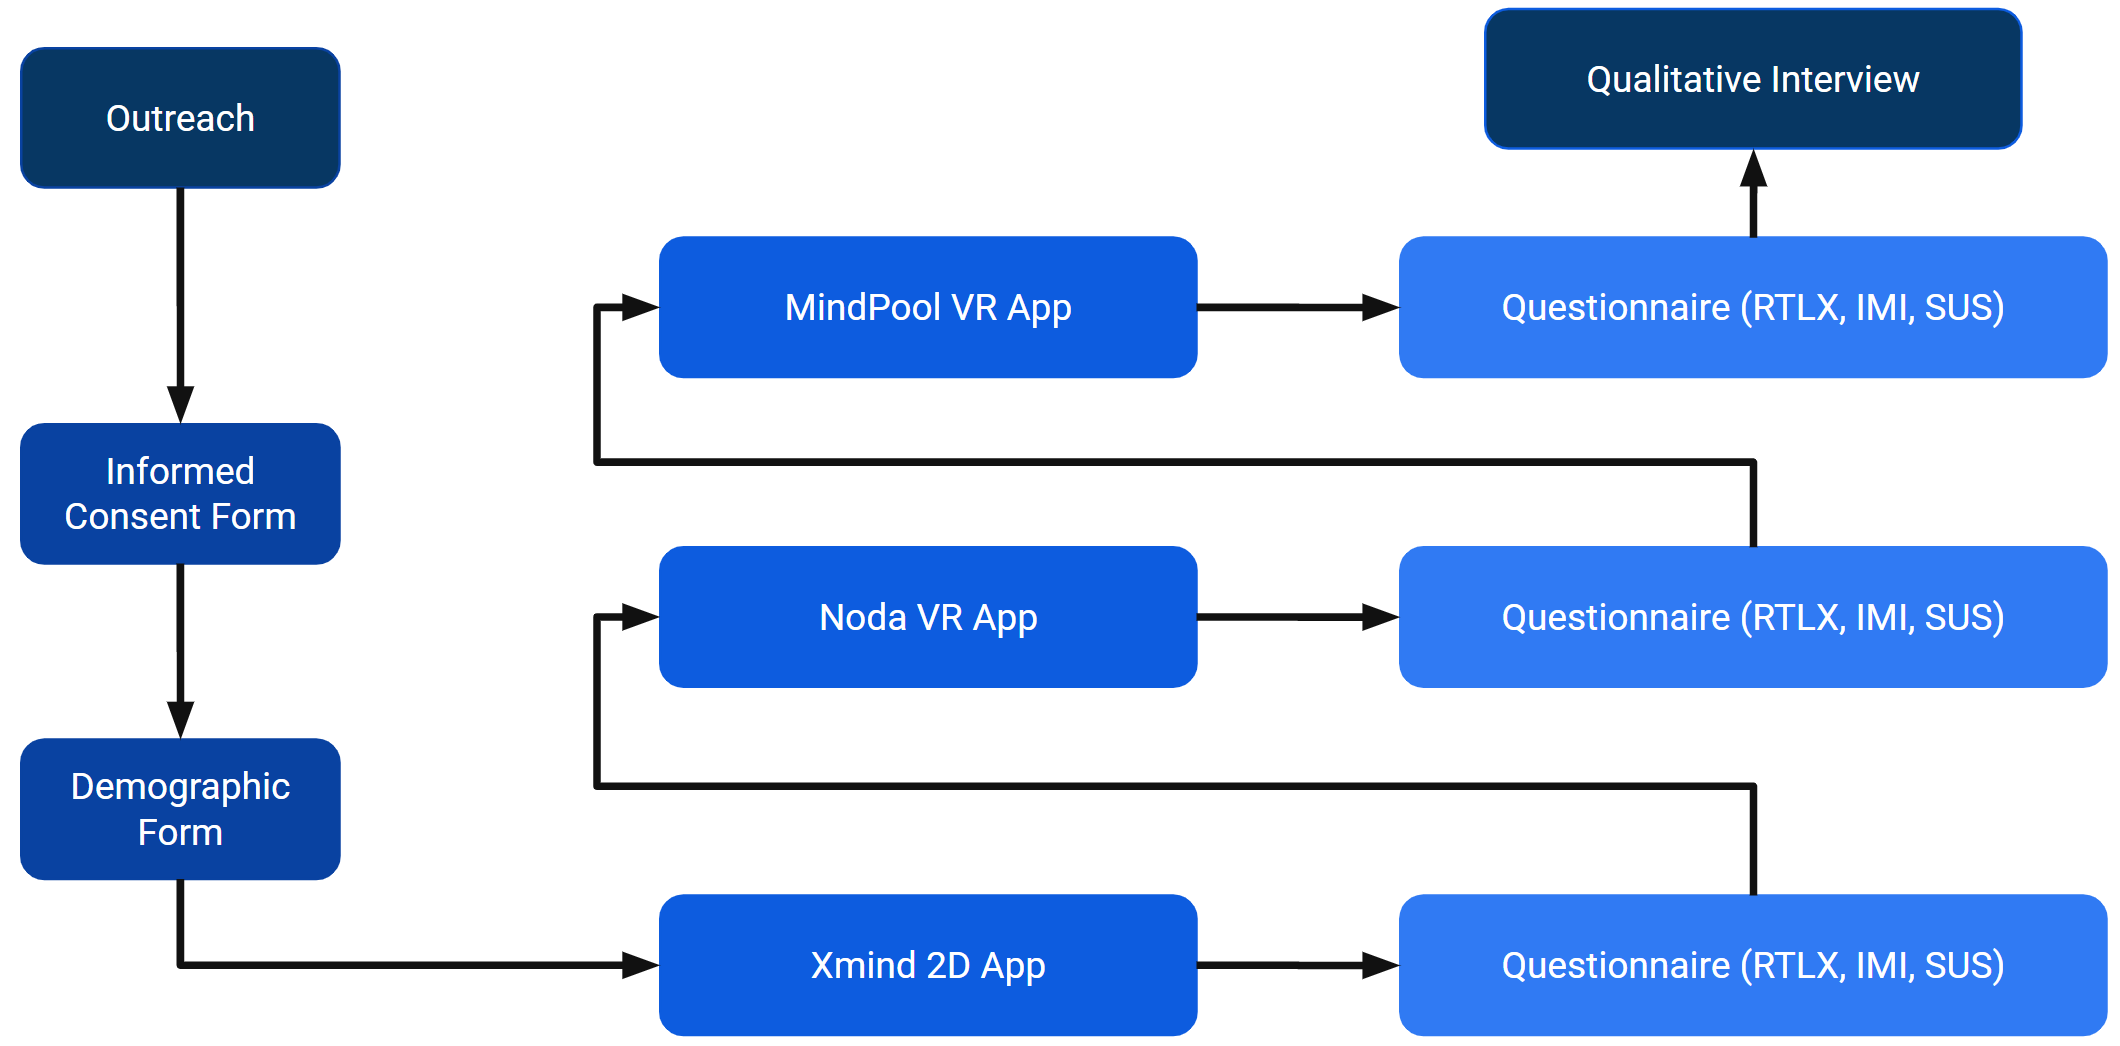
\includegraphics[width=1\linewidth]{fig/Exp_Design.png}
    \caption{Experimental Design Flow}
    \label{fig:Exp_Design}
\end{figure}

\subsection{Task Description}
Participants were assigned a structured, standardized mind mapping task designed to simulate a practical information organization scenario. The task involved:
\begin{enumerate}
    \item Researching top-rated restaurants in Chicago using an in-app or external browser.
    \item Creating a hierarchical mind map starting with a central node titled "Chicago."
    \item Adding two child nodes, each representing the names of two restaurants found via Google search.
    \item For each restaurant node, adding two dish nodes representing selected menu items, with an additional information under each dish listing its price.
    \item Structuring all nodes into a tree-like top-down hierarchy to ensure consistency across conditions.
    \item Creating the connections between nodes to form a mind map
    \item Answering two analytic questions based on the completed map:
    \begin{enumerate}
        \item "Which dish was the cheapest?"
        \item "Which dish was the most expensive?"
    \end{enumerate}
\end{enumerate}
The mind mapping procedure was kept identical across all three apps, ensuring that task complexity and cognitive demands remained consistent.

% \begin{figure}[h!]
%   \centering
%   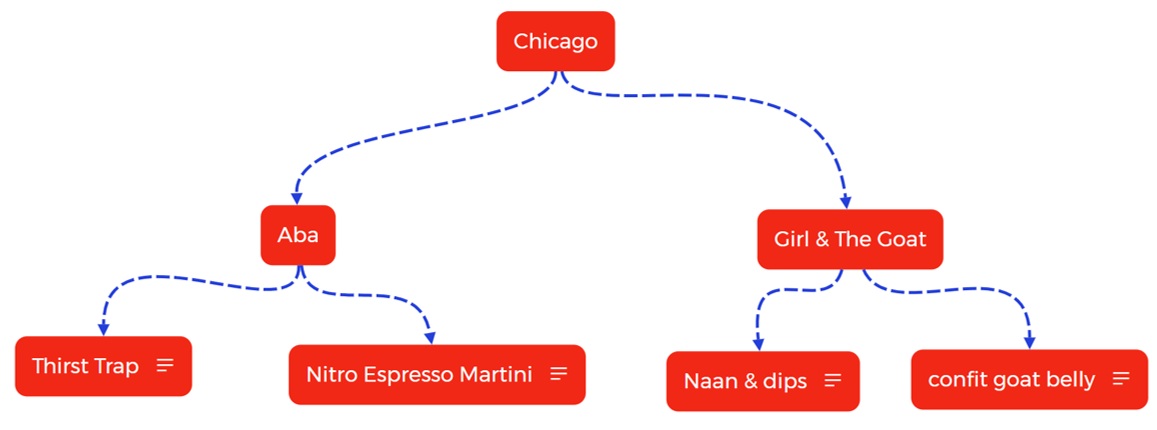
\includegraphics[width=0.32\textwidth]{fig/ss_xmind/2D_task.png} % Adjust width
%   \hfill
%   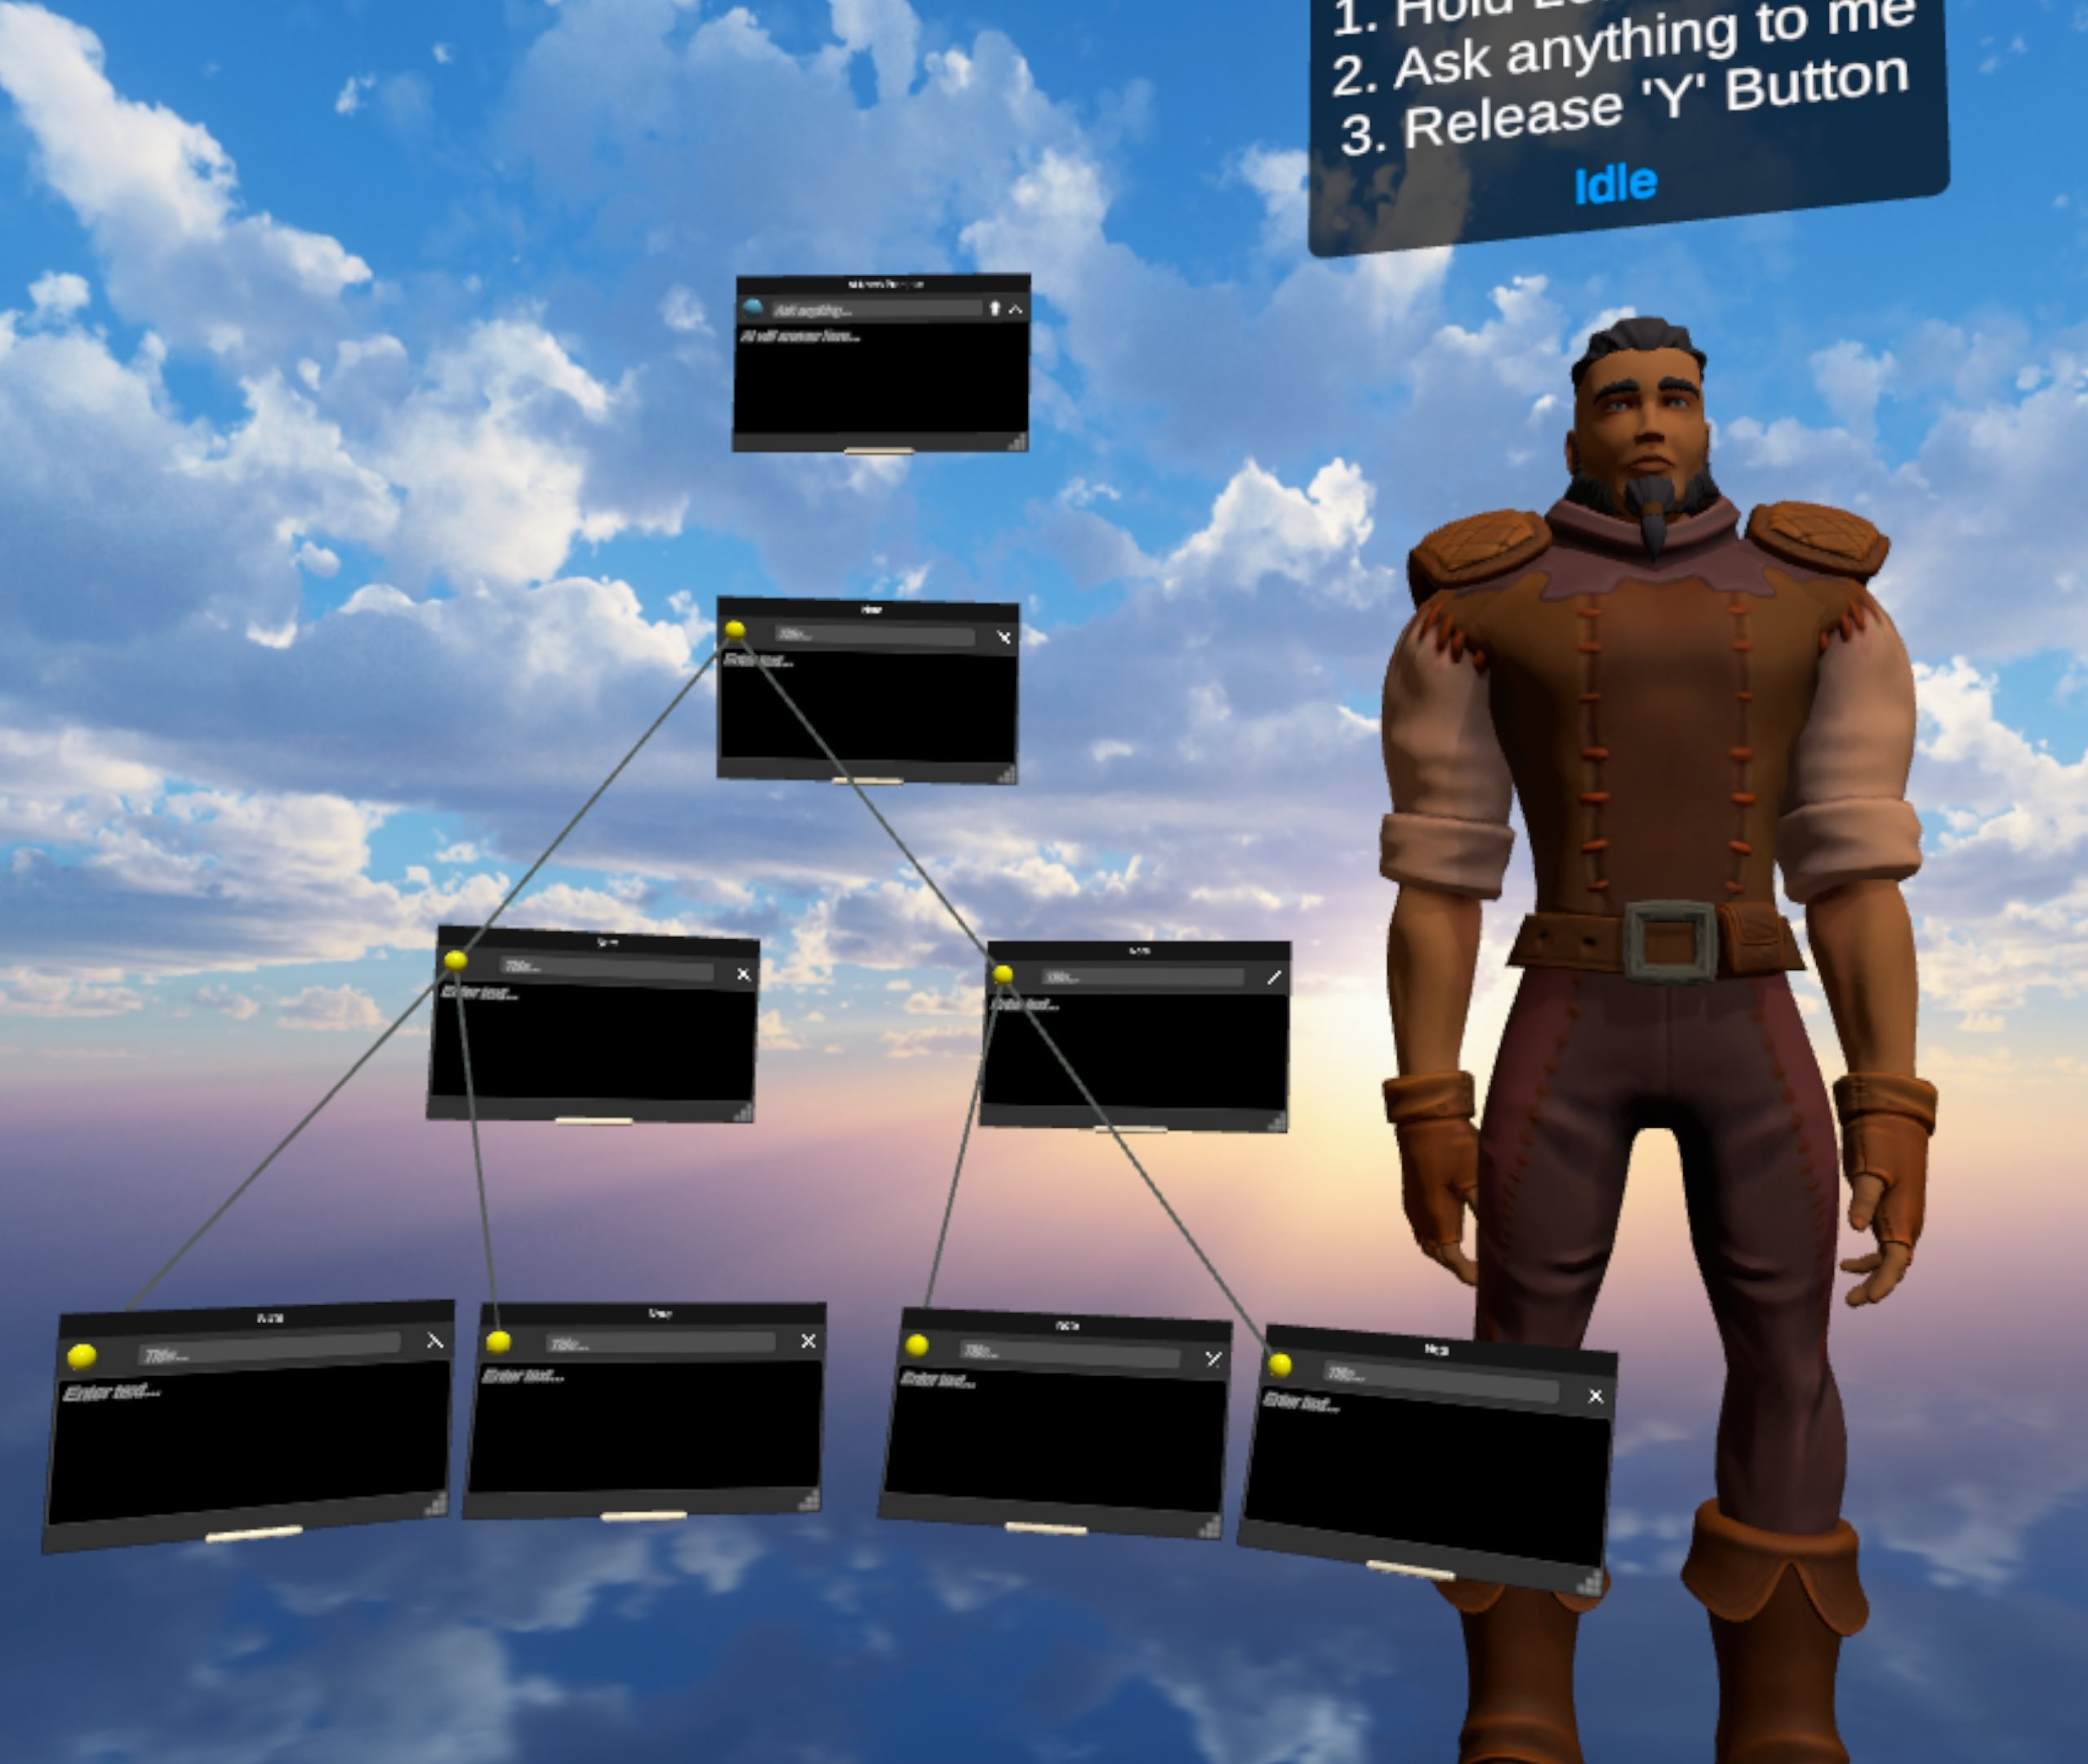
\includegraphics[width=0.32\textwidth]{fig/ss_mindpool/MP_task2.jpg} % Adjust width
%   \hfill
%   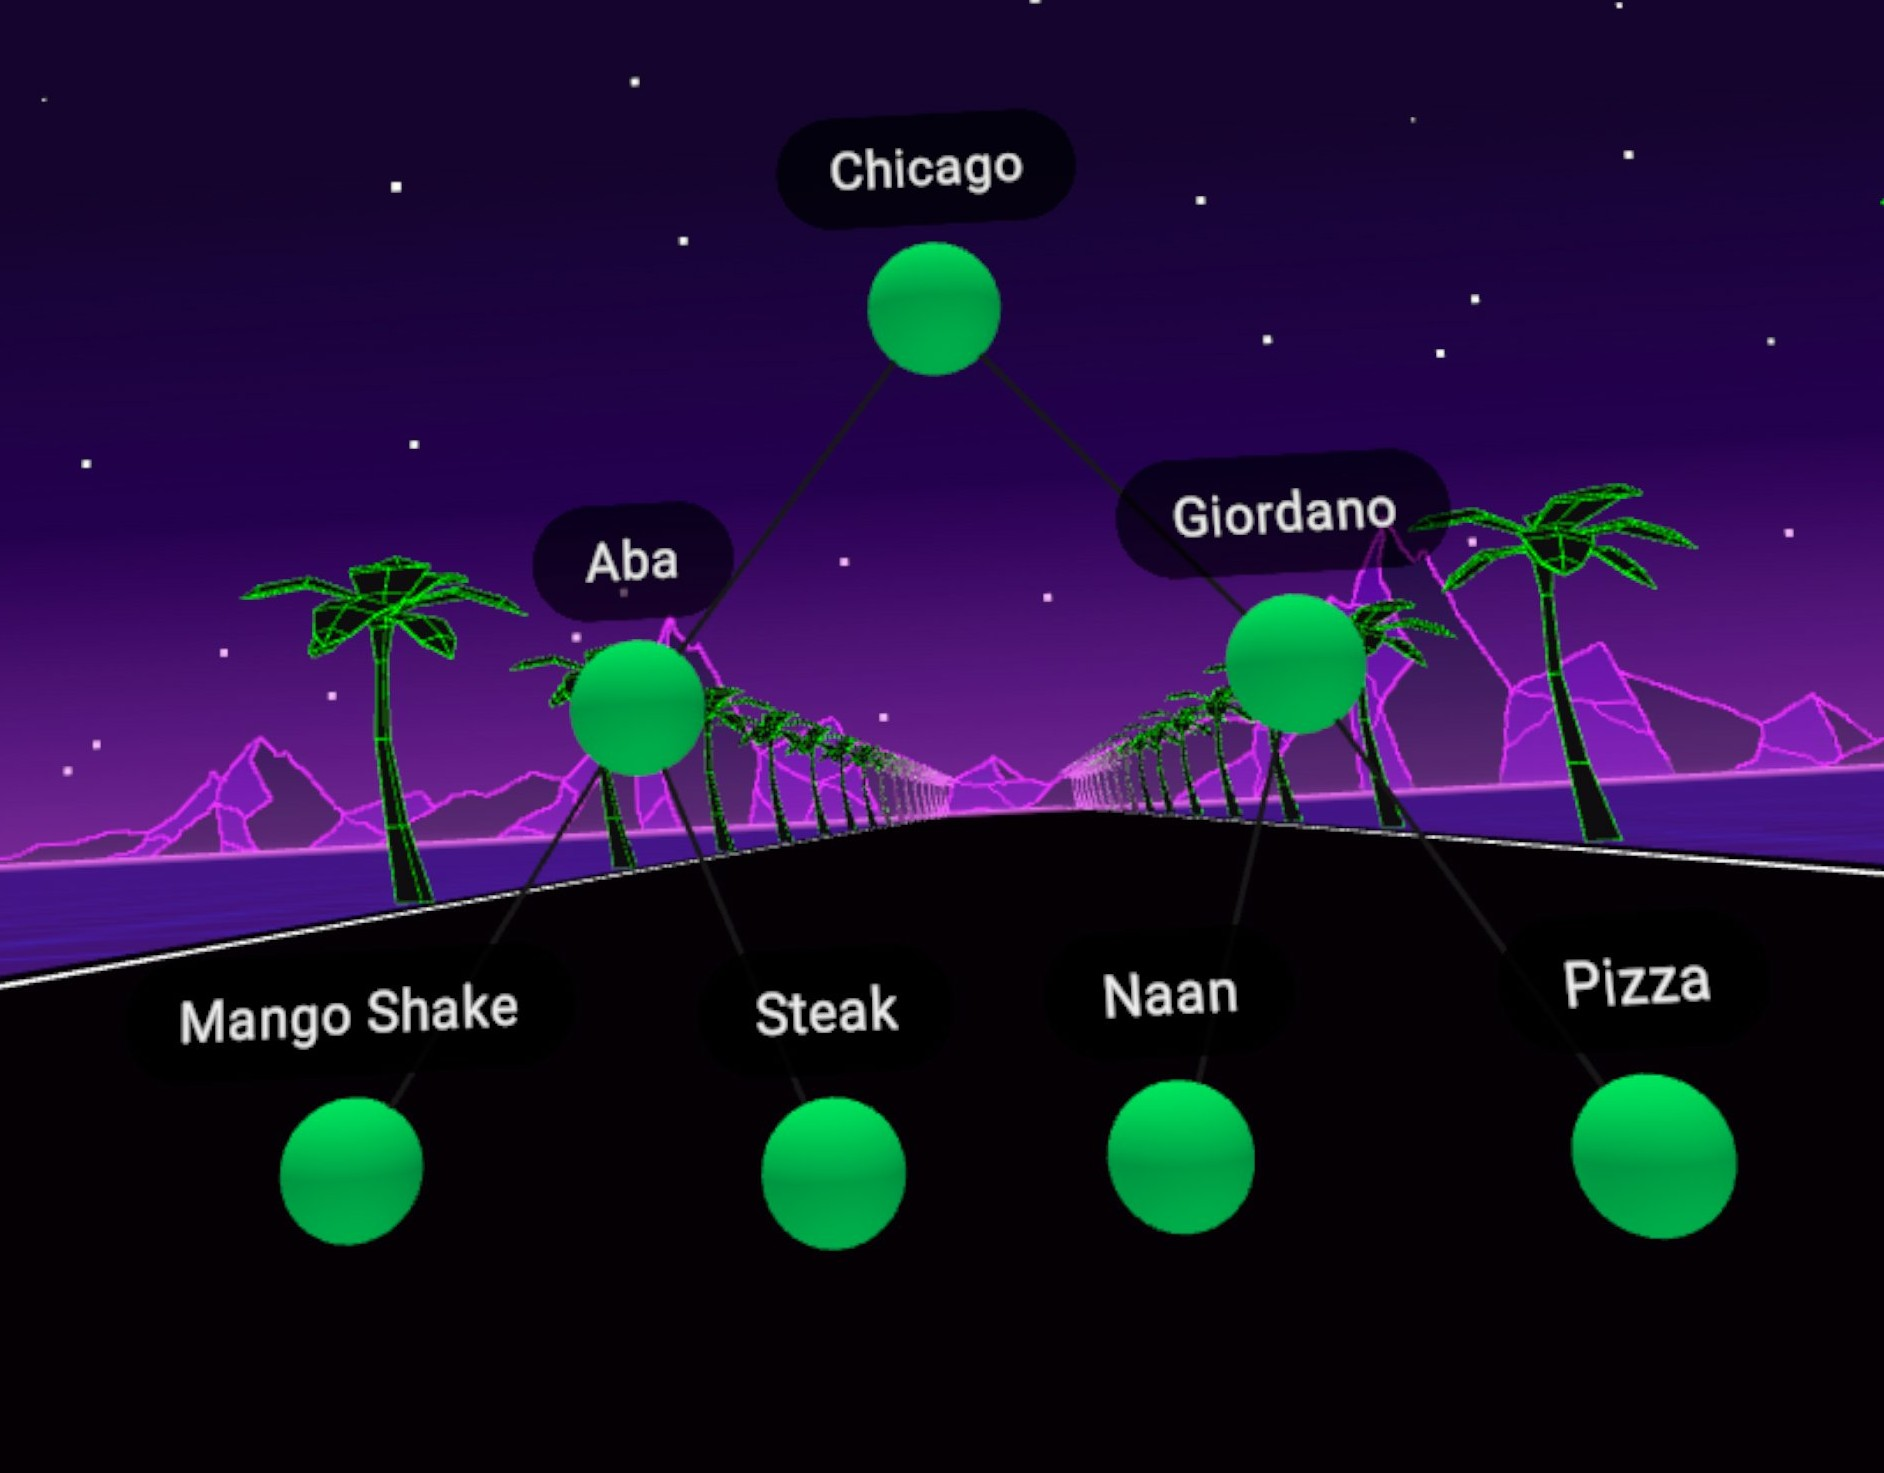
\includegraphics[width=0.32\textwidth]{fig/ss_noda/Noda_task2.jpg} % Adjust width
%   \caption{Three images side by side}
%   \label{fig:threeimages}
% \end{figure}

\begin{figure}[h!]
  \centering
  \begin{subfigure}{\textwidth} % Top image spans the full width
    \centering
    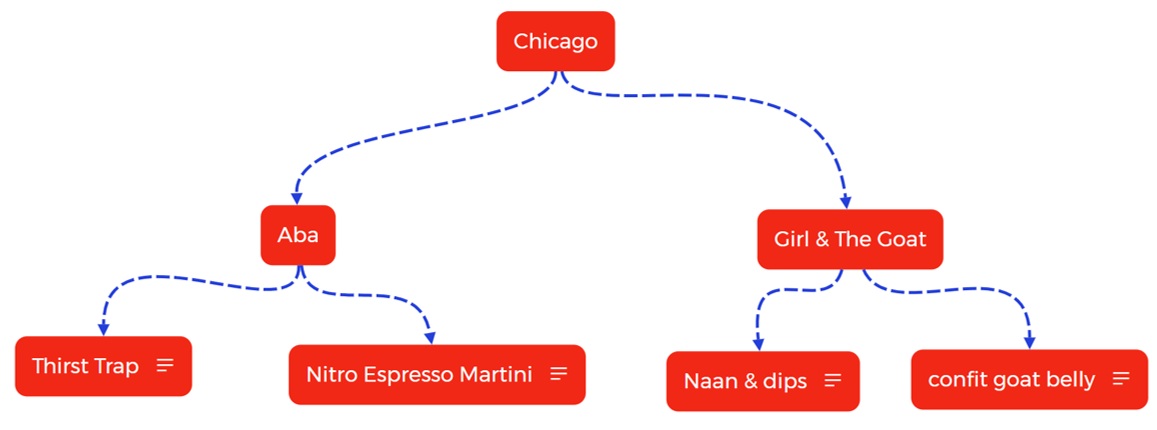
\includegraphics[width=0.5\textwidth]{fig/ss_xmind/2D_task.png} % Adjust width as needed
    \caption{Xmind (2D)}
    \label{fig:top}
  \end{subfigure}
  \bigskip % Add vertical space between the top and bottom rows

  \begin{subfigure}{0.48\textwidth} % First image in the bottom row
    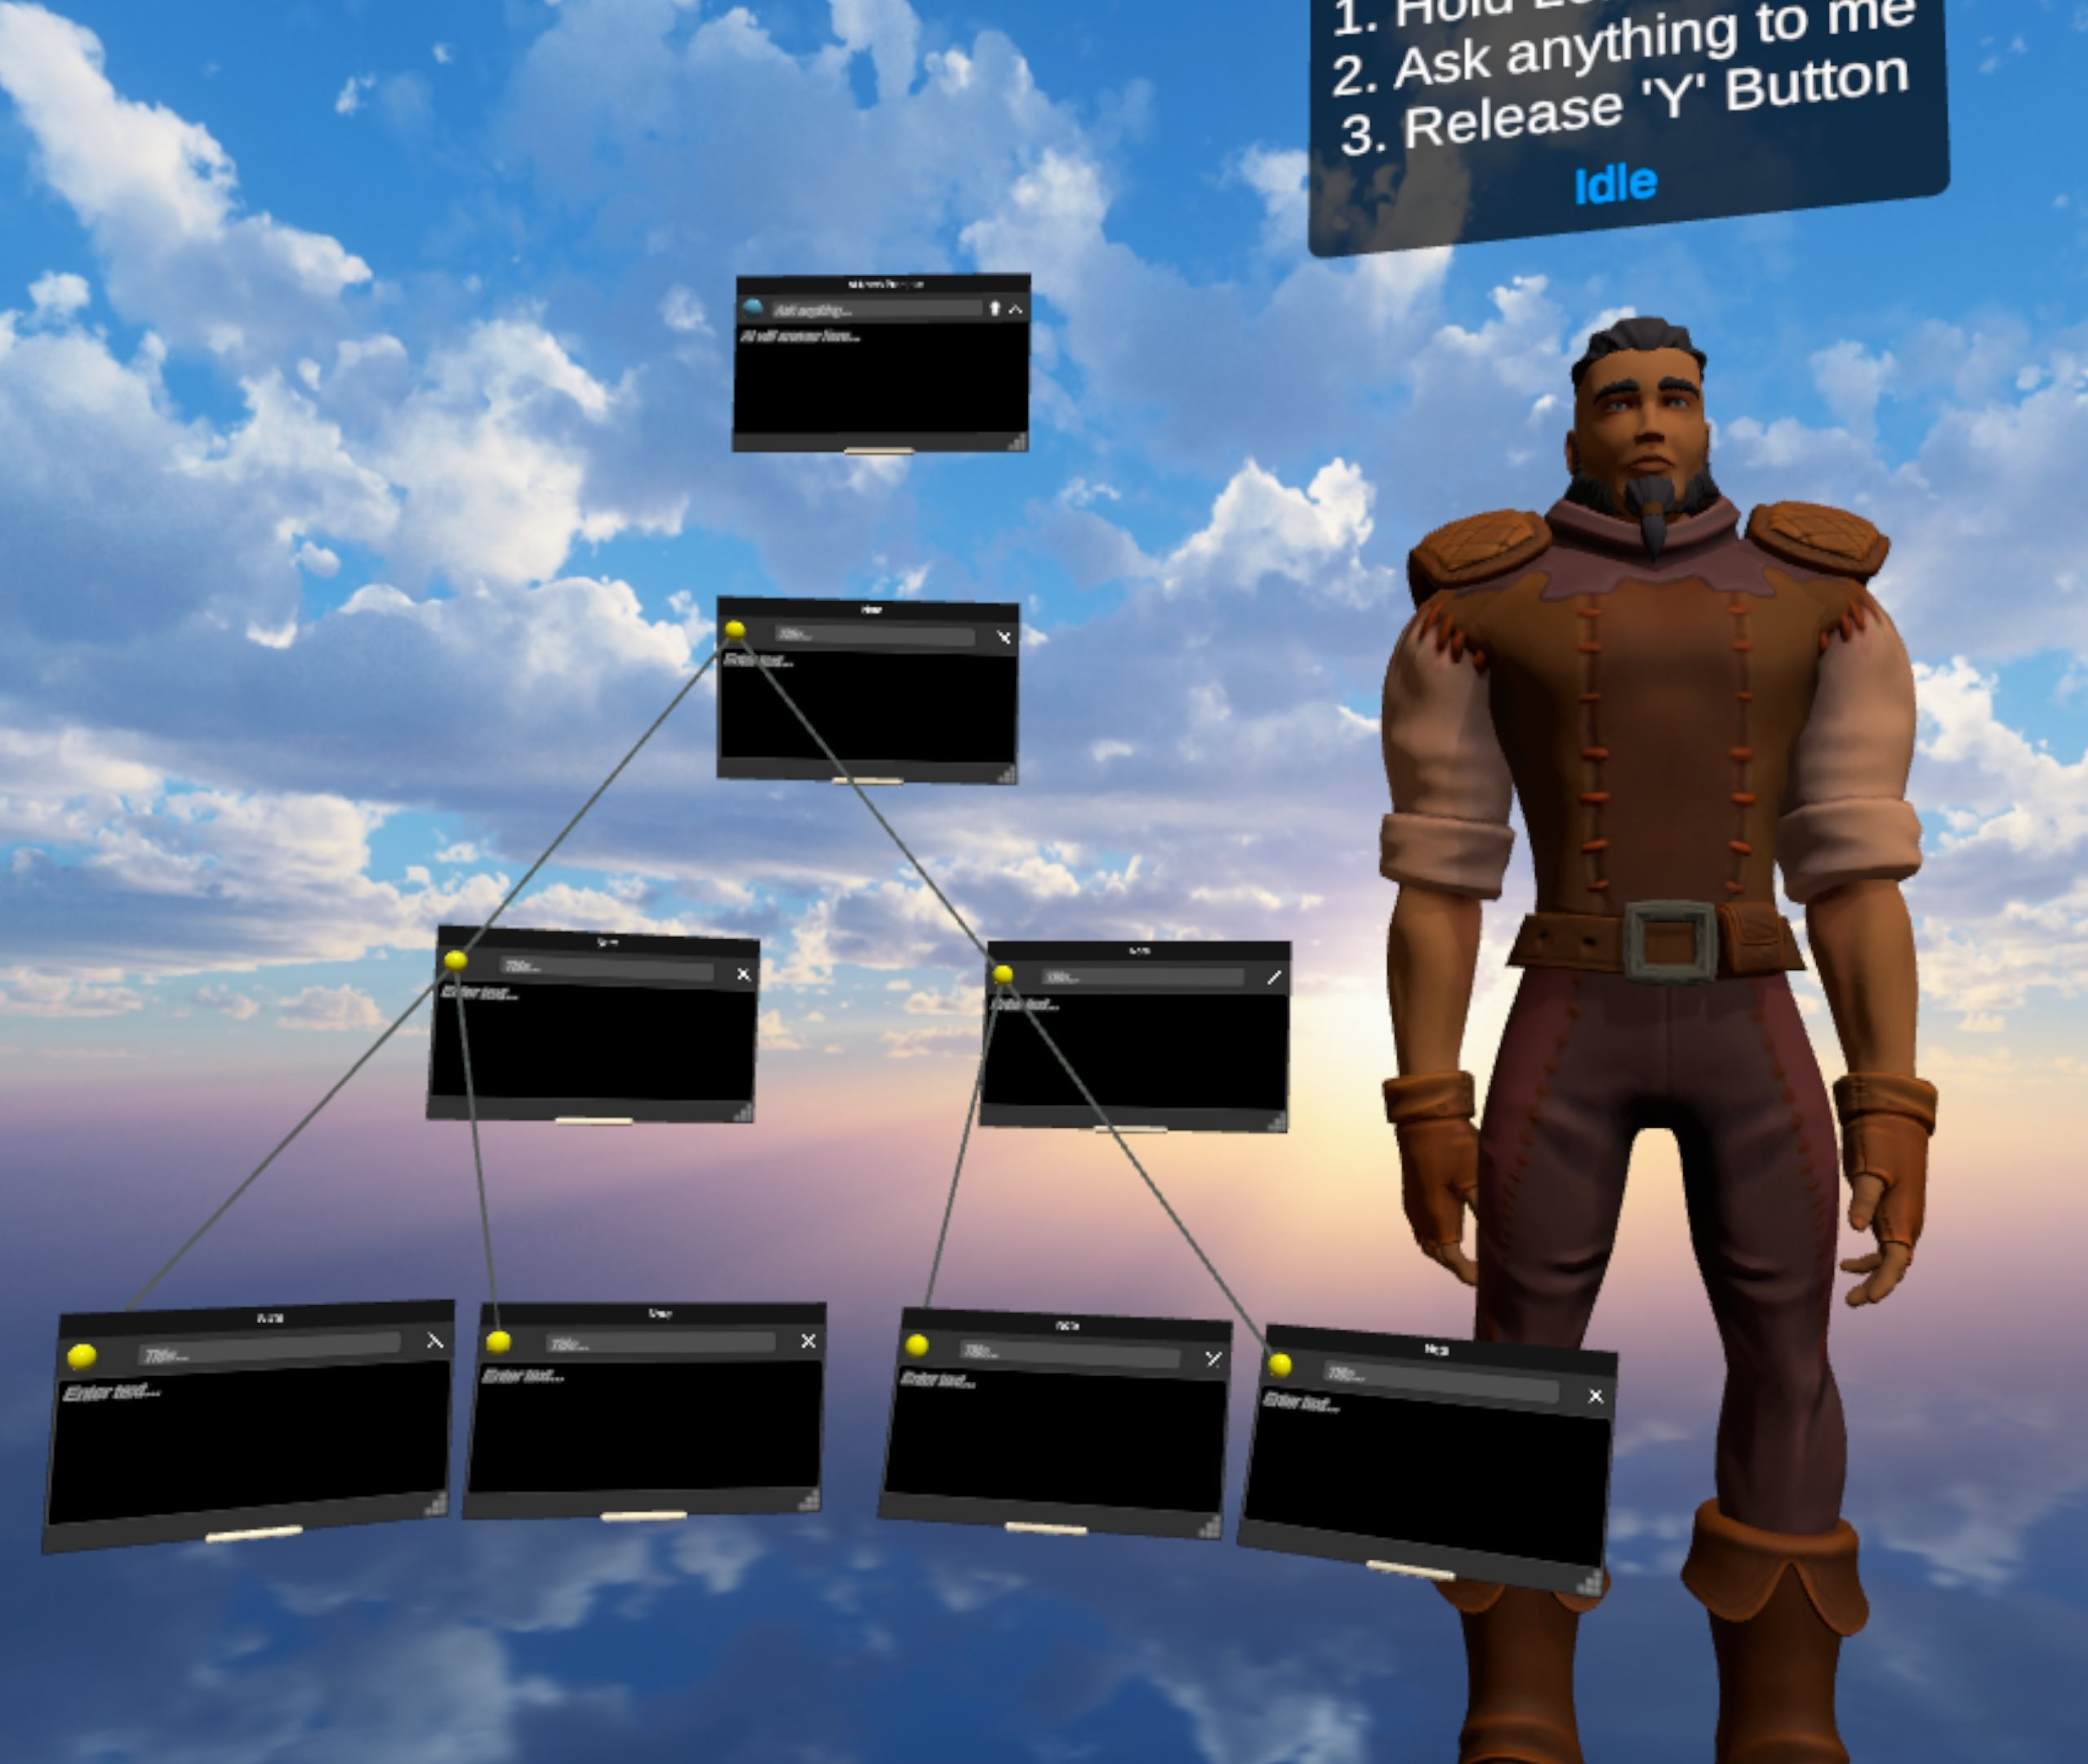
\includegraphics[width=\textwidth]{fig/ss_mindpool/MP_task2.jpg}
    \caption{MindPool (VR)}
    \label{fig:bottomleft}
  \end{subfigure}
  \hfill
  \begin{subfigure}{0.48\textwidth} % Second image in the bottom row
    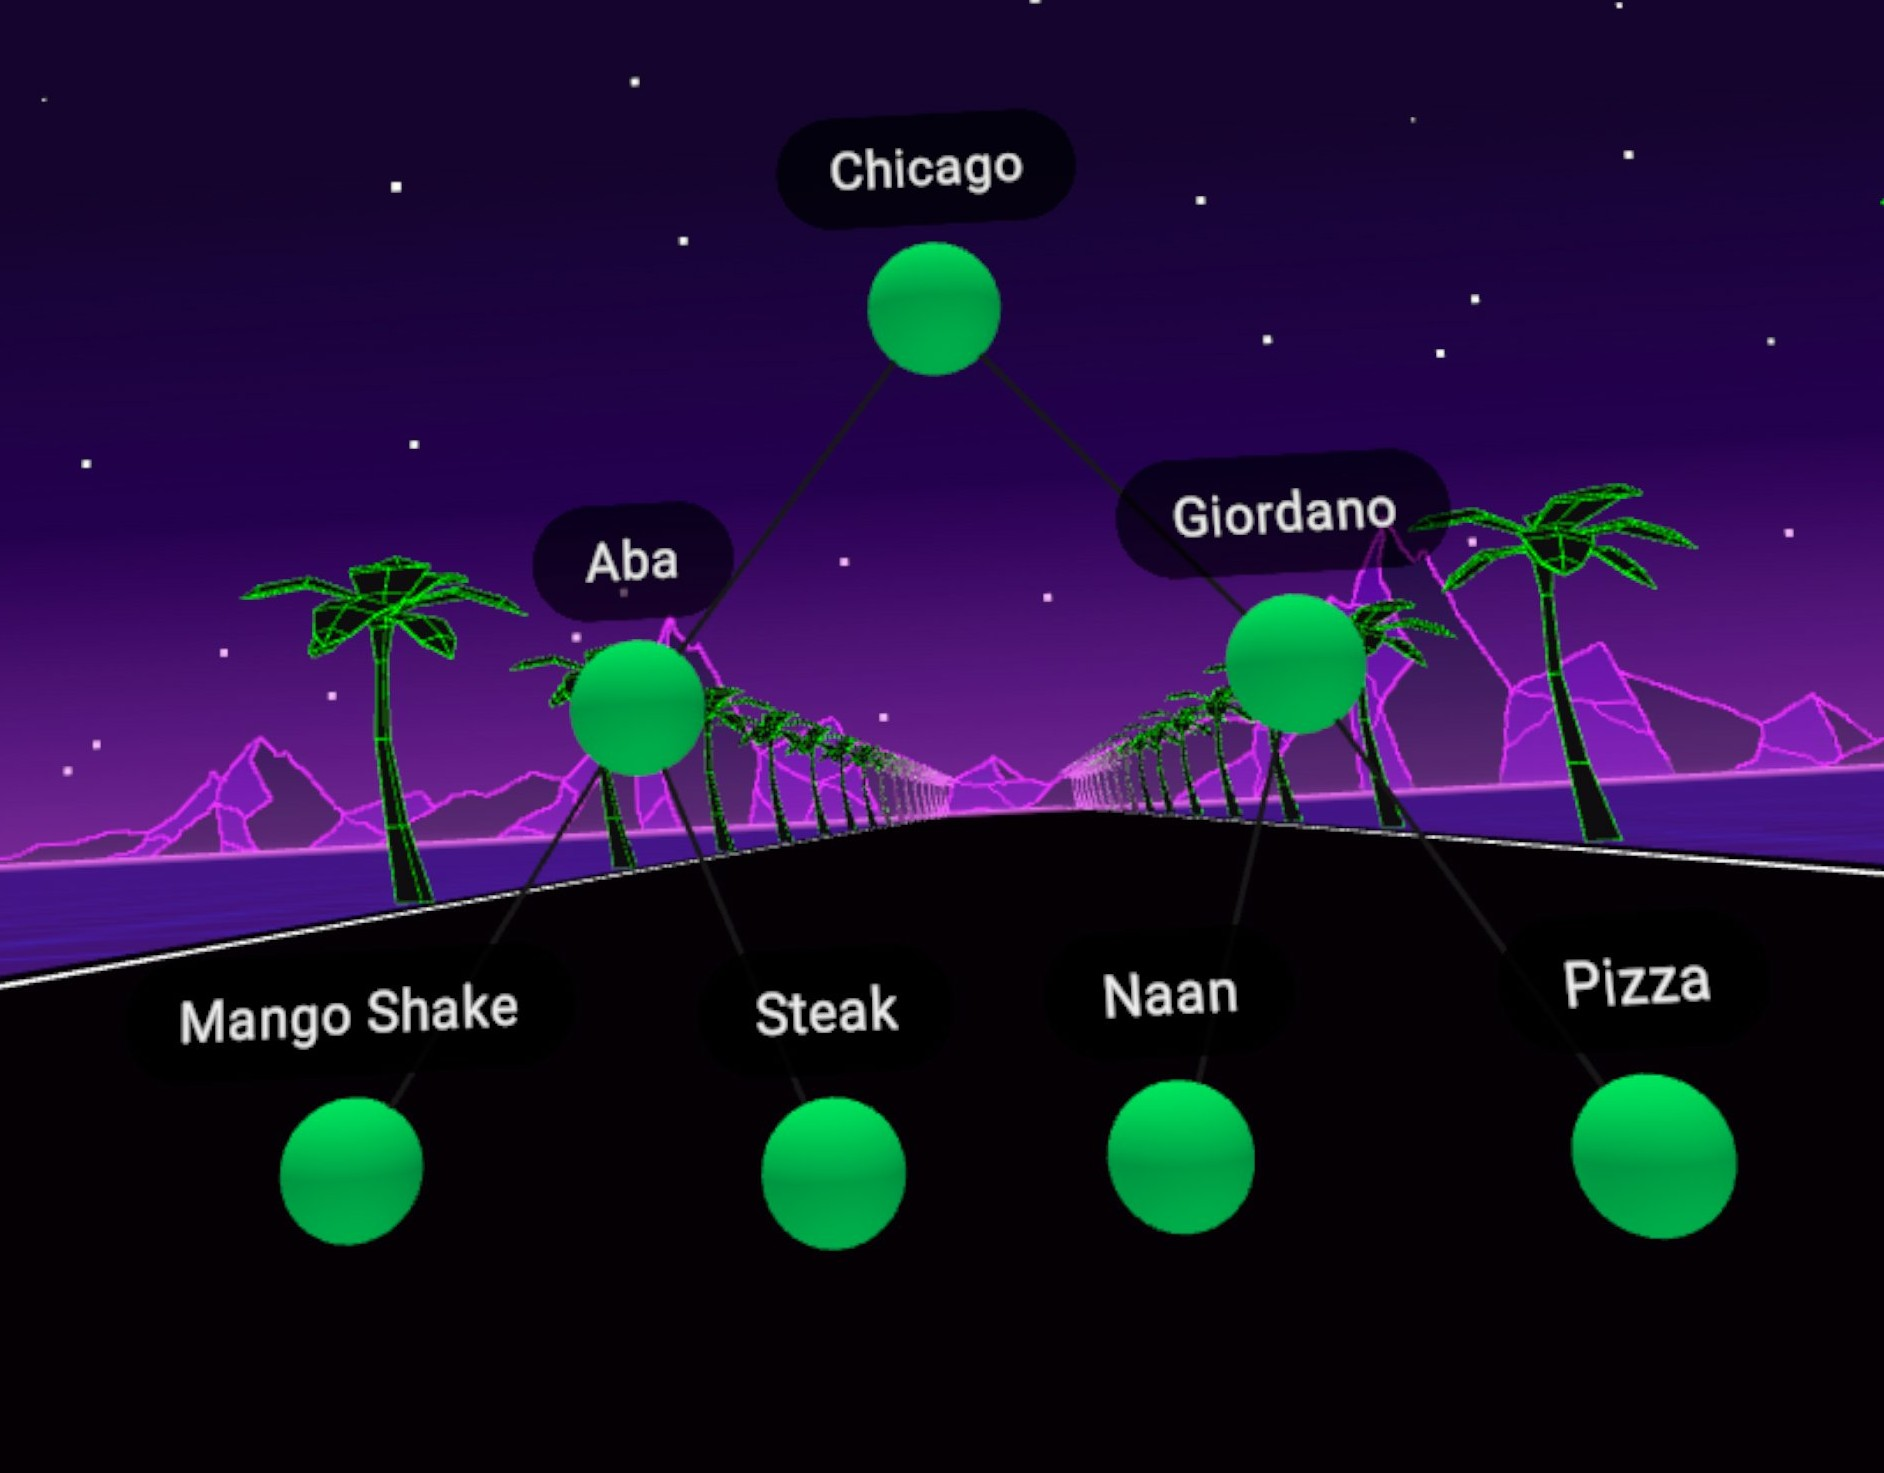
\includegraphics[width=\textwidth]{fig/ss_noda/Noda_task2.jpg}
    \caption{Noda (VR)}
    \label{fig:bottomright}
  \end{subfigure}

  \caption{Screenshots of the tasks completed by participants in each app}
  \label{fig:combined_arrangement}
\end{figure}

\subsection{Platform Conditions}
\begin{itemize}
    \item XMind v25.01.01061 (2D Desktop App): Participants completed the mind map using the XMind desktop application on a standard monitor and keyboard setup.
    \item MindPool (XR App with AI Enhancements): Participants used the MindPool app with AI-enabled features (AI Note and Conversational Avatar) available but not required for task completion.
\end{itemize}

\subsection{Counterbalancing to Mitigate Order Effects}
To control for potential learning, fatigue, or novelty effects, participants were randomly assigned into three counterbalanced groups:
\begin{itemize}
    \item Group 1: 2D (XMind) → XR (MindPool) → XR (Noda)
    \item Group 2: XR (Noda) → XR (MindPool) → 2D (XMind)
    \item Group 3: XR (MindPool) → XR (Noda) → 2D (XMind)
\end{itemize}
Each group contained a mix of male and female participants to maintain gender balance across conditions.

\subsection{Session Flow}
Each app session consisted of:
\begin{enumerate}
    \item A brief familiarization or tutorial segment (2-10 depending on app).
    \item The main restaurant mind mapping task (5-20 minutes depending on app).
    \item Post-task questionnaire completion (RTLX, IMI, SUS).
    \item Physiological data recording throughout the task phases.
\end{enumerate}
The total session time per participant was approximately 1 to 1.5 hours, including setup, breaks, debriefing, and qualitative interviews.



\section{Data Collection}

Data collection in this study followed a multi-method approach, combining physiological measurements, standardized questionnaires, and qualitative feedback to comprehensively assess participant experience across the three app conditions (XMind, Noda, MindPool).


\subsection{Participant Data}

A total of 10 participants (5 male, 5 female) were recruited for this study. Participants were recruited through a combination of word-of-mouth communication and posts in student Discord groups targeting university and college communities. Interested individuals contacted the research team and were screened for eligibility. No financial incentive or course credit was provided; participation was entirely voluntary.

\begin{table}[h!]
\centering
\begin{tabular}{|p{1cm}|p{1cm}|p{2cm}|p{2cm}|p{2cm}|p{2cm}|p{1cm}|p{2cm}|}
\hline
Id & Age & Gender & Education & Experience with VR & Experience with Computers & Hours using VR last month & Hours creating mindmaps last month\\ \hline
1 & 23 & Female & Master's & Quite a bit & Quite a bit & 5 & 1 \\ \hline
2 & 22 & Female & Bachelor's & Slightly & Very much & 0 & 0 \\ \hline
3 & 25 & Female & Master's & Quite a bit & Very much & 1 & 0 \\ \hline
4 & 20 & Male & Bachelor's & Slightly & Very much & 1 & 1 \\ \hline
5 & 23 & Female & Bachelor's & Neutral & Quite a bit & 0 & 0 \\ \hline
6 & 25 & Female & Master's & Not at all & Very much & 0 & 0 \\ \hline
7 & 20 & Male & Bachelor's & Slightly & Very much & 0 & 0 \\ \hline
8 & 23 & Male & Master's & Slightly & Very much & 0 & 0 \\ \hline
9 & 20 & Male & Bachelor's & Very much & Very much & 20 & 0 \\ \hline
10 & 25 & Male & Master's & Quite a bit & Very much & 4 & 2 \\ \hline
\end{tabular}
\caption{Participant's Demographic}
\label{table:demographic}
\end{table}

Participants were required to be fluent in English and have no known motor, visual, or cognitive impairments that would affect their ability to complete the experimental tasks. Prior experience with XR devices or mind mapping tools was not required, as the study aimed to evaluate usability across a general user base.

\subsubsection{Demographic Overview}

Participants varied in age, educational background, and familiarity with VR technology. Before starting the study, participants completed a demographic questionnaire that collected information on their age, gender, handedness, VR experience, and prior use of mind mapping tools.
A detailed list of participants’ ages, genders, current education, and experiences with VR, computers, and mind mapping can be found in Table~\ref{table:demographic}. As all participants were predominantly right-handed, handedness was not presented as a variable in the table.


\subsubsection{Group Assignment and Counterbalancing}

To control for potential order effects—such as learning, fatigue, or novelty—participants were randomly assigned to one of three counterbalanced groups:

\begin{itemize}
    \item Group 1 (n=3): XMind → MindPool → Noda
    \item Group 2 (n=3): Noda → MindPool → XMind
    \item Group 3 (n=4): MindPool → Noda → XMind
\end{itemize}

Each group included a mix of male and female participants to maintain gender balance. The counterbalanced structure ensured that each application (2D and XR) was experienced in every possible order position across the participant pool, thereby minimizing systematic bias.

\subsubsection{Ethical Compliance}

All participants provided written informed consent before participation, in accordance with IRB-approved protocols. Participants were briefed about the study objectives, experimental procedures, their right to withdraw at any time without penalty, and the confidentiality measures employed to protect their data. Personal identifiers were anonymized during data analysis to ensure privacy.

\subsection{Physiological Data}

Physiological signals were collected using the Biopac Research Ring, a wearable sensor device worn on the left-hand index finger of each participant. The following signals were continuously recorded:

\begin{itemize}
    \item Heart Rate (HR) and Heart Rate Variability (HRV) via photoplethysmography (PPG)
    \item Electrodermal Activity (EDA) for sympathetic nervous system activation
    \item Skin Temperature (SKT) for peripheral thermal response monitoring
\end{itemize}

Physiological data were recorded only during the task phase for each app, corresponding to the 10-minute period when participants were actively engaged in creating their mind maps. A separate physiological recording session was initiated for each application to ensure clear data segmentation and prevent cross-condition contamination.

All physiological signals were securely stored for post-processing and feature extraction as detailed in Section 3.5.

\subsection{Questionnaire Data}

After completing the task in each app, participants completed a set of three validated questionnaires:

\begin{itemize}
    \item NASA Raw Task Load Index (RTLX): Assessed subjective workload across six dimensions (Mental Demand, Physical Demand, Temporal Demand, Performance, Effort, Frustration).
    \item Intrinsic Motivation Inventory (IMI): Evaluated user motivation through subscales measuring Interest/Enjoyment, Perceived Competence, Effort/Importance, and Pressure/Tension. 
    \item System Usability Scale (SUS): Measured perceived ease of use, satisfaction, and learnability.
\end{itemize}

Questionnaires were administered electronically immediately after each task to capture fresh impressions and minimize recall bias.

\subsection{Qualitative Data}

At the end of the experimental session, participants provided open-ended qualitative feedback through guided interview questions:

\begin{enumerate}
    \item Which app did you find most enjoyable and why?
    \item Which app was the easiest to use and why?
    \item Which app was the easiest to get started with, including finding a tutorial, learning how to use it, and understanding its features on your own?
    \item In which app did you feel it was easiest to organize your thoughts without feeling overwhelmed and will use regularly? Will your answer change if you were to make a much larger and complicated mind map?
    \item Did you find the AI features (AI Note, AI Avatar) useful in improving your mind mapping experience? How did interacting with the AI avatar (speaking/listening) compare to traditional typing or browsing?
    \item What did you like or dislike about each app, and if you could add or change one feature to improve your favorite app, what would it be?
\end{enumerate}

Additionally, spontaneous verbal remarks made by participants during the sessions were noted. These observations included comments on ease of use, system responsiveness, interface design, and any usability frustrations or appreciations.

Qualitative responses were later analyzed thematically to supplement and contextualize the quantitative data.

\section{Signal Processing}

Physiological data collected during the task phases were analyzed to extract insights into participants’ cognitive load and engagement. Due to signal quality observations and preliminary inspection, only PPG-derived heart rate variability (HRV) analysis was carried forward for detailed investigation.

\subsection{Heart Rate Variability (HRV) Analysis}

The primary physiological metric used in this study was heart rate variability (HRV), derived from photoplethysmography (PPG) signals recorded by the Biopac Research Ring. Data acquisition and analysis were performed using AcqKnowledge software (BIOPAC Systems, Inc.).

HRV is a measure of the variation in time intervals between consecutive heartbeats, often used as an indicator of autonomic nervous system activity. One commonly used time-domain HRV metric is the Root Mean Square of Successive Differences (RMSSD), which quantifies short-term variability by measuring the magnitude of variability between successive inter-beat intervals (IBIs) \cite{taskforce1996}. RMSSD is calculated as follows:

\[
\text{RMSSD} = \sqrt{ \frac{1}{N-1} \sum_{i=1}^{N-1} (IBI_{i+1} - IBI_i)^2 }
\]

where \( IBI_i \) represents the time interval (in milliseconds) between successive PPG peaks. This metric is particularly sensitive to parasympathetic (vagal) activity and is widely used to assess stress and cognitive load.

Although HRV can be computed manually by detecting peaks in the PPG signal, calculating inter-beat intervals, and then applying the above formula, AcqKnowledge provides an automated solution. The software performs preprocessing steps internally—including bandpass filtering, peak detection, artifact rejection, and IBI computation—once the HRV analysis function is activated. This allows for consistent and efficient analysis across sessions.

\begin{itemize}
    \item \textbf{Focus Area Selection:} For each participant and each app session, a specific focus area was manually selected within AcqKnowledge, corresponding precisely to the time window during which the participant was actively performing the mind mapping task (excluding tutorial phases).
    \item \textbf{Automated HRV Analysis:} Using AcqKnowledge’s built-in HRV analysis module, key HRV metrics were automatically computed over the selected task focus areas. Extracted features included:
    \begin{itemize}
        \item Mean Heart Rate (in beats per minute)
        \item Root Mean Square of Successive Differences (RMSSD) (in milliseconds)
    \end{itemize}
\end{itemize}

These HRV analysis results were then used to compare physiological responses across the three app conditions (XMind, Noda, MindPool), offering insights into differences in user stress and cognitive load during the mind mapping tasks.


\subsection{Electrodermal Activity (EDA) and Skin Temperature (SKT)}

During the experiment, we recorded electrodermal activity (EDA) and skin temperature (SKT) signals in addition to our primary modalities. While the SKT data exhibited minimal variation across sessions and participants, suggesting limited utility for our current research questions, the EDA data presented a different challenge. Although collected, a thorough analysis of the EDA signals was not undertaken within the scope of this thesis. This decision was primarily driven by the need for further investigation into reliable and appropriate analytical methodologies that align with our specific research objectives, a process that extended beyond the current project timeline. Consequently, to maintain a focused analysis on our core research questions, both EDA and SKT data were excluded from the final analysis presented herein. We believe that future research endeavors should prioritize the application of suitable analytical methods to the collected EDA signals, potentially uncovering valuable insights that complement the findings of this study.

\section{Ethical Consideration}

All procedures conducted in this study adhered to ethical standards for research involving human participants. Institutional Review Board (IRB) approval was obtained prior to the commencement of participant recruitment and data collection.

Before participation, each individual was provided with a detailed informed consent form outlining the purpose of the study, the procedures involved, potential risks and benefits, the voluntary nature of participation, and confidentiality assurances. Participants were informed that they could withdraw from the study at any time without any penalty or loss of benefits.

To protect participant privacy, no personally identifiable information was collected beyond basic demographic data (e.g., age range, gender, VR experience level), and all data were anonymized prior to analysis. Physiological data, questionnaire responses, and qualitative feedback were stored securely on password-protected systems accessible only to the authorized researchers.

Participants were also informed that there would be no financial compensation for participation and that the study was purely voluntary. Any questions or concerns raised by participants before, during, or after the study were addressed promptly and respectfully.

\newpage

\chapter{Results}

\section{Questionnaire Analysis}



\subsection{Descriptive Statistics}

Descriptive statistics were calculated for each questionnaire category—Cognitive Load (RTLX), Intrinsic Motivation (IMI), and Usability (SUS)—across the three apps: XMind (2D), Noda (VR), and MindPool (custom VR) and are shown in Figure~\ref{fig:rtlx-breakdown},~\ref{fig:imi-breakdown},~\ref{fig:sus-usability}.

\begin{figure}[hbt!]
    \centering
    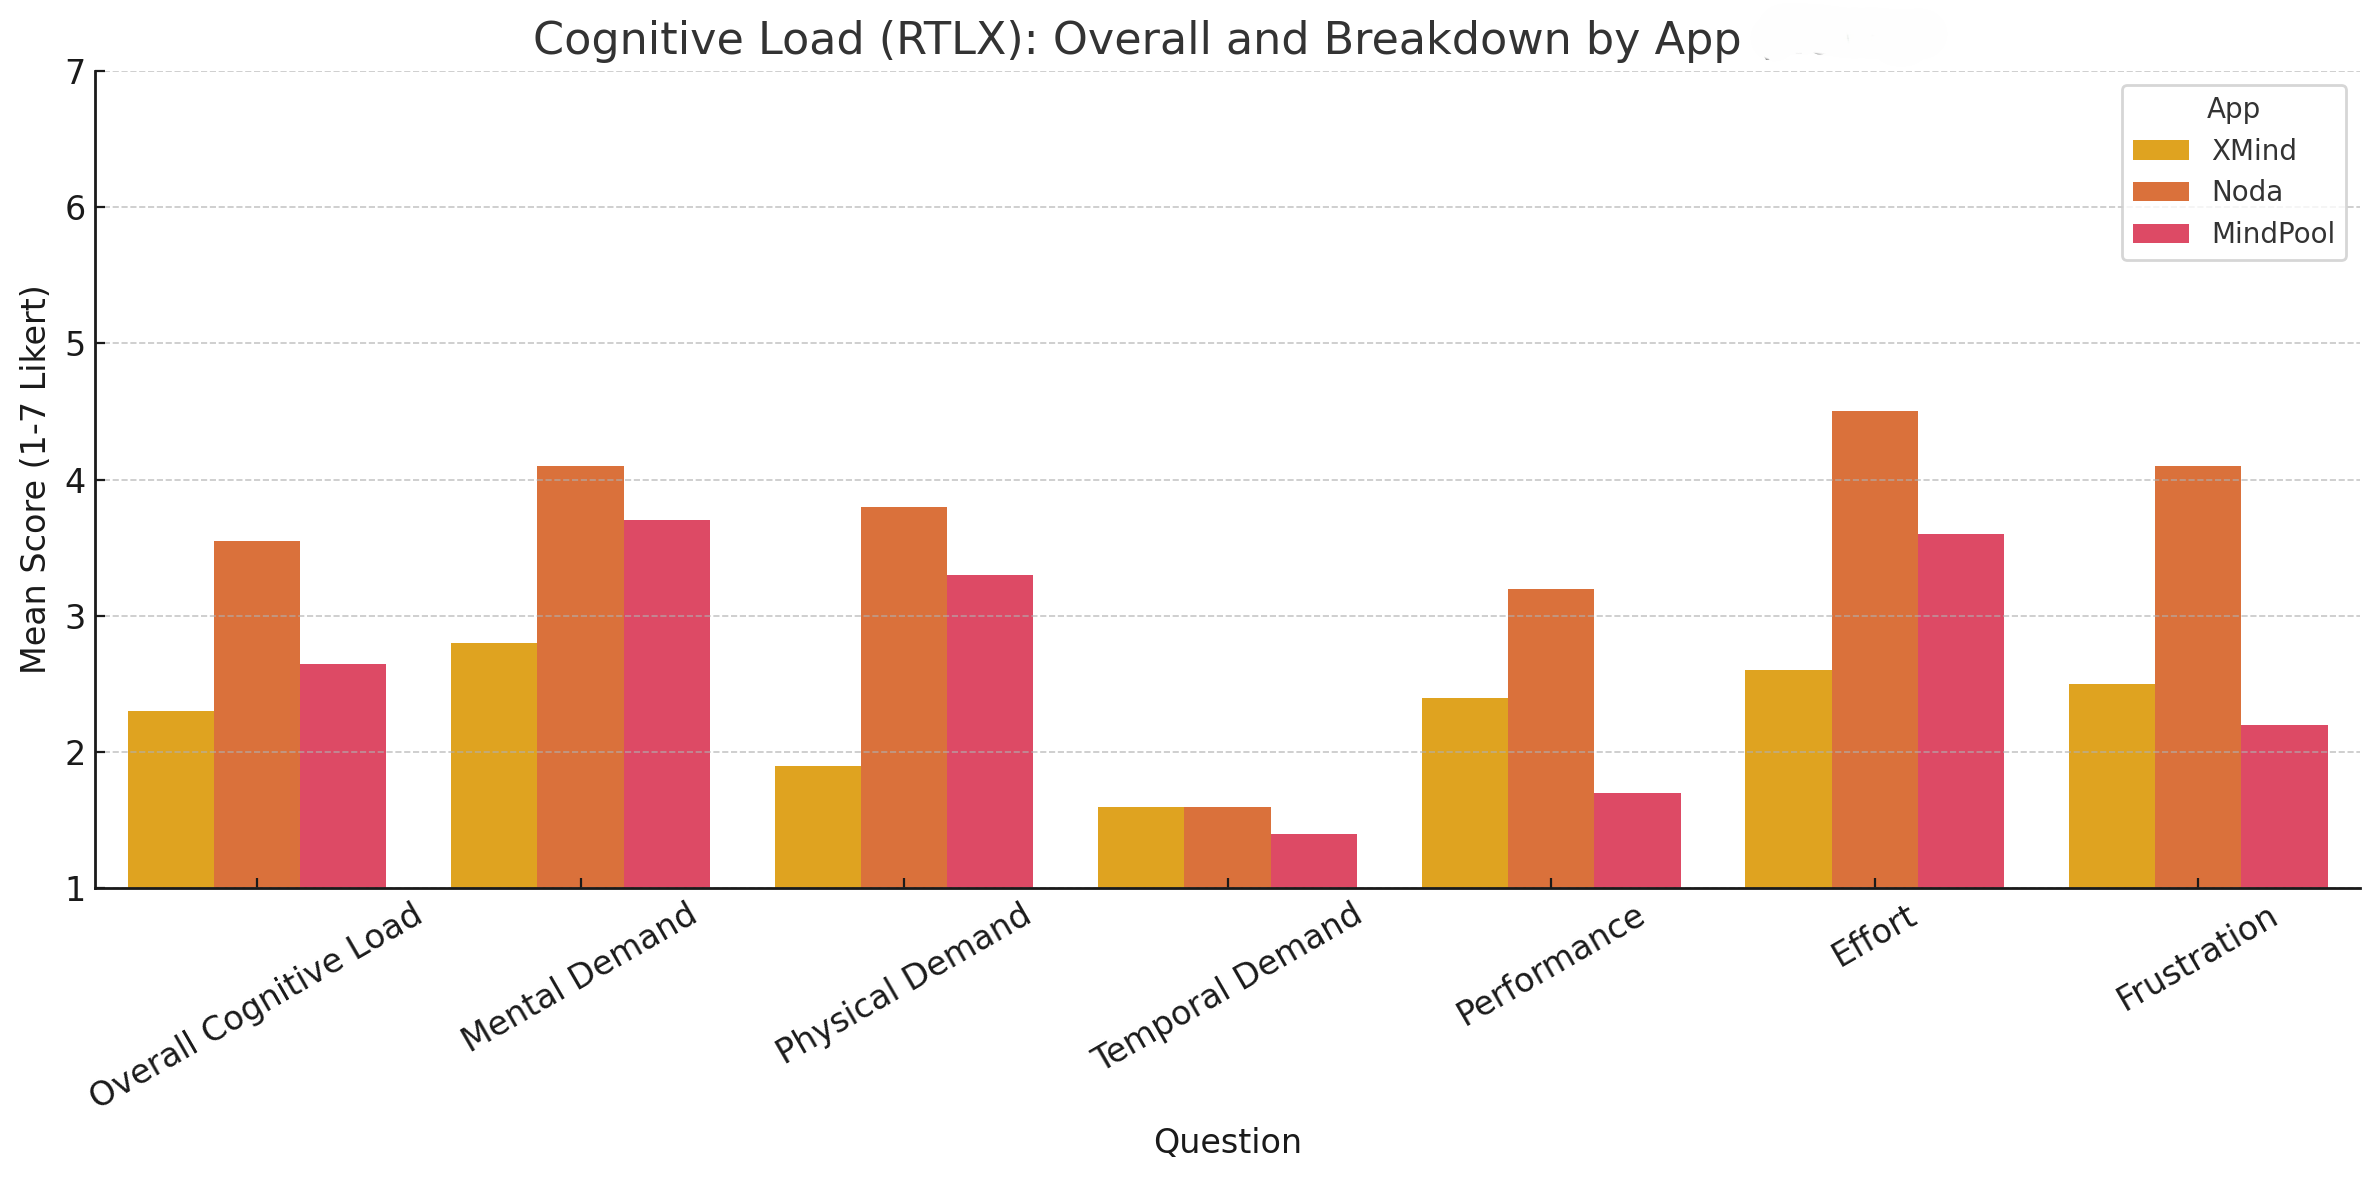
\includegraphics[width=\textwidth]{fig/Questionnaire/rtlx.png}
    \caption{Cognitive Load (RTLX): Overall and Breakdown by App}
    \label{fig:rtlx-breakdown}
\end{figure}

In terms of cognitive load, XMind consistently received the lowest scores across both the overall RTLX composite and most individual subscales, indicating the lowest perceived mental and physical burden among the three apps. In contrast, Noda yielded the highest cognitive load ratings across all dimensions, suggesting it imposed the greatest cognitive demands. MindPool fell between the two: its overall cognitive load score was closer to XMind, while its mental demand, physical demand, and effort scores were more similar to Noda. However, for performance and frustration, MindPool's scores aligned more closely with XMind. These results suggest that MindPool offers a balanced cognitive experience, combining elements of both 2D and VR interaction in a way that potentially mitigates the drawbacks of each.

\begin{figure}[hbt!]
    \centering
    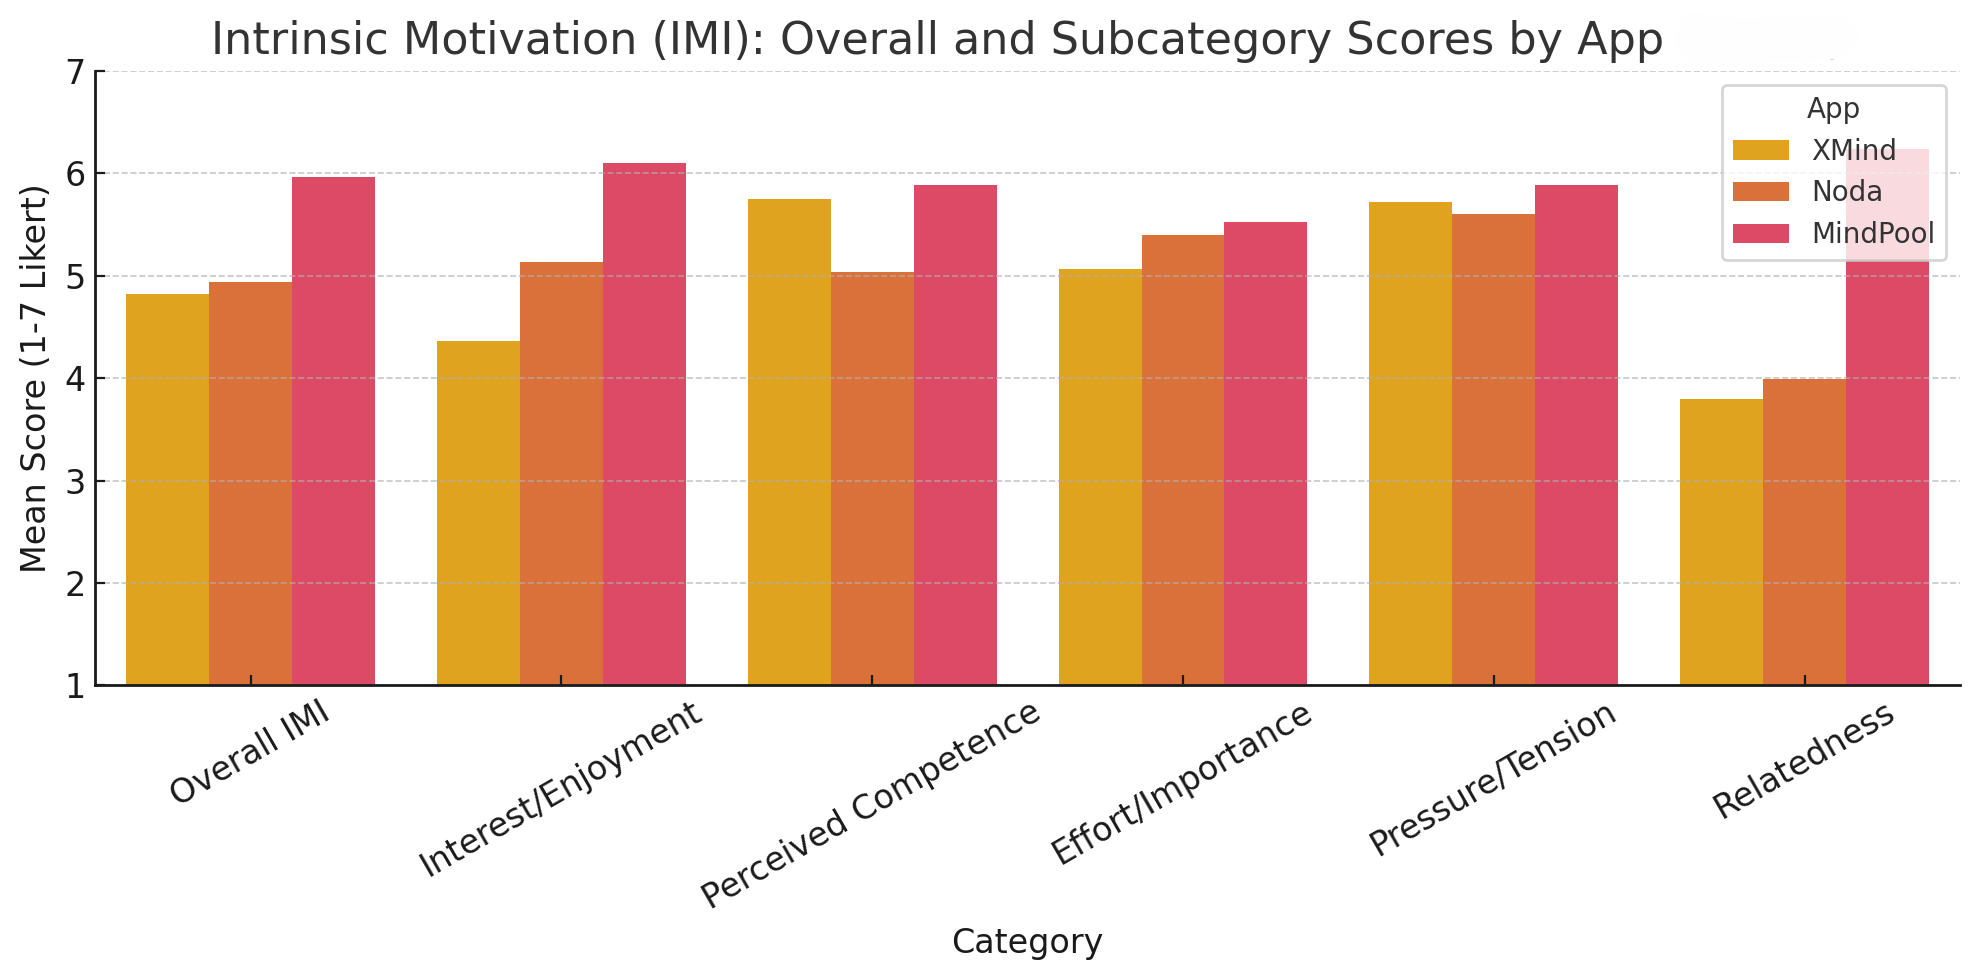
\includegraphics[width=\textwidth]{fig/Questionnaire/imi.png}
    \caption{Intrinsic Motivation (IMI): Overall and Subcategory Scores by App}
    \label{fig:imi-breakdown}
\end{figure}

In the domain of intrinsic motivation, MindPool consistently received the highest ratings across the IMI subscales, indicating greater levels of user engagement, enjoyment, and perceived competence. XMind, while performing well in terms of cognitive simplicity, showed the lowest motivational scores, suggesting that its traditional 2D format may offer less stimulating or immersive experiences. Noda generally ranked between the two, though it occasionally scored the lowest in subcategories such as relatedness and perceived competence. These patterns highlight MindPool’s strength in fostering user motivation through enhanced interactivity and immersive features, while also suggesting potential engagement limitations in the more conventional 2D interface of XMind. 

\begin{figure}[hbt!]
    \centering
    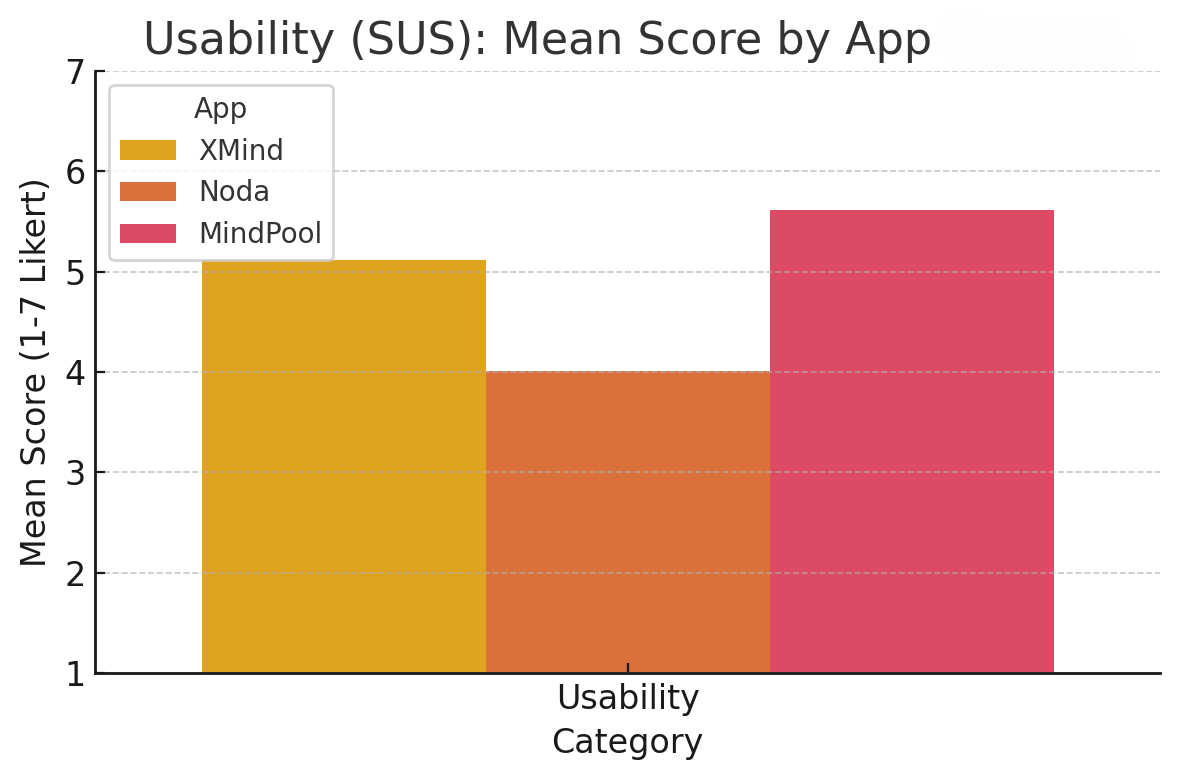
\includegraphics[width=0.6\textwidth]{fig/Questionnaire/sus.png}
    \caption{Usability (SUS): Mean Score by App}
    \label{fig:sus-usability}
\end{figure}

Regarding usability, MindPool received the highest average SUS scores, suggesting it was perceived as the most intuitive and functionally integrated app. XMind followed closely behind, indicating that its familiar 2D interface was also generally well-received in terms of ease of use. Noda, by contrast, scored the lowest, reflecting greater perceived complexity or inconsistency in user interaction. These findings highlight the effect of the usability enhancements introduced in MindPool and suggest that it is one step closer to bridging the gap between immersive VR functionality and user-friendly design.


\subsection{Inferential Statistics}

To examine whether the observed differences in questionnaire responses between XMind, Noda, and MindPool were statistically significant, Friedman tests were conducted for each main category and subcategory. The results are shown in Table~\ref{tab:friedman-results}.

\begin{table}[h!]
    \centering
    \caption{Friedman Test Results for Questionnaire Subscales}
    \label{tab:friedman-results}
    \begin{tabular}{|c|c|c|p{2.2cm}|}
        \hline
        \textbf{Category} & \textbf{Friedman Statistic} & \textbf{$p$ - value} & \textbf{Significant ($p < 0.05$)} \\
        \hline
        RTLX (Cognitive Load) - Overall & 6.200 & 0.045 & Yes \\
        RTLX - Mental Demand & 4.563 & 0.102 & No \\
        RTLX - Physical Demand & 4.788 & 0.091 & No \\
        RTLX - Temporal Demand & 1.333 & 0.513 & No \\
        RTLX - Performance & 6.897 & 0.032 & Yes \\
        RTLX - Effort & 4.563 & 0.102 & No \\
        RTLX - Frustration & 3.722 & 0.156 & No \\
        IMI (Intrinsic Motivation) - Overall & 12.760 & 0.002 & Yes \\
        IMI - Interest/Enjoyment & 18.200 & 0.00011 & Yes \\
        IMI - Perceived Competence & 6.722 & 0.035 & Yes \\
        IMI - Effort/Importance & 4.563 & 0.102 & No \\
        IMI - Pressure/Tension & 3.722 & 0.156 & No \\
        IMI - Relatedness & 8.000 & 0.018 & Yes \\
        SUS (Usability) - Overall & 7.200 & 0.027 & Yes \\
        \hline
    \end{tabular}
\end{table}

\textbf{Interpretation:}

Statistically significant differences were observed across several key categories, providing evidence that participants' experiences varied meaningfully between the three apps.

\begin{itemize}
    \item \textbf{Cognitive Load (RTLX)} differed significantly across the apps ($\chi^2 = 6.20$, $p = 0.045$), suggesting that users perceived distinct differences in mental workload depending on the interface. Notably, the subcategory \textbf{Performance} also showed significance ($p = 0.032$), indicating that users’ satisfaction with their own task performance was influenced by the app they used.
    
    \item Other subscales of RTLX, such as mental demand, effort, and frustration, did not reach significance. This may be due to high inter-participant variability or a limited sample size, which can reduce statistical power. Still, the presence of significant differences in overall RTLX and performance underscores that perceived cognitive burden is a meaningful differentiator.

    \item \textbf{Intrinsic Motivation (IMI)} showed the most robust differences. Overall motivation was highly significant ($p = 0.002$), and subscales including \textbf{Interest/Enjoyment} ($p < 0.001$), \textbf{Perceived Competence} ($p = 0.035$), and \textbf{Relatedness} ($p = 0.018$) revealed that participants were more engaged, felt more capable, and felt better supported by some apps than others. This suggests that differences in design and interactivity directly impact users’ intrinsic motivation.

    \item The \textbf{Usability (SUS)} scores also revealed significant differences ($p = 0.027$), affirming that not all interfaces were equally intuitive or easy to use. Given that SUS is widely used in HCI evaluations, this finding reinforces that usability remains a major factor in user satisfaction and task performance.

    \item The lack of significant differences in subscales like temporal demand and pressure/tension may be due to the fact that all participants completed very similar, well-structured tasks. Because the experience was controlled and predictable, participants likely felt neither rushed nor anxious, resulting in similar scores across all apps
\end{itemize}

These findings collectively suggest that MindPool’s improvements over Noda—especially in motivational design and usability—were impactful, and that 2D interfaces like XMind may still offer cognitive efficiency, though possibly at the expense of user engagement.


\subsection{Post-hoc Analysis}

For each questionnaire category where the Friedman test indicated a statistically significant difference between apps, Wilcoxon signed-rank tests were conducted to identify where those differences occurred. The full results are presented in Table~\ref{tab:wilcoxon-results}.

\begin{table}[h!]
    \centering
    \caption{Post-hoc Wilcoxon Test Results for Significant Categories}
    \label{tab:wilcoxon-results}
    \begin{tabular}{|c|c|p{2cm}|c|c|}
        \hline
        \textbf{Category} & \textbf{Comparison} & \textbf{Wilcoxon Statistic} & \textbf{p-value} & \textbf{Significant} \\
        \hline
        RTLX - Overall & XMind vs Noda & 4.0 & 0.014 & Yes \\
        RTLX - Overall & XMind vs MindPool & 14.5 & 0.193 & No \\
        RTLX - Overall & Noda vs MindPool & 9.5 & 0.084 & No \\
        RTLX - Performance & XMind vs Noda & 8.0 & 0.293 & No \\
        RTLX - Performance & XMind vs MindPool & 5.0 & 0.121 & No \\
        RTLX - Performance & Noda vs MindPool & 10.0 & 0.105 & No \\
        IMI - Overall & XMind vs Noda & 1.0 & 0.005 & Yes \\
        IMI - Overall & XMind vs MindPool & 1.0 & 0.005 & Yes \\
        IMI - Overall & Noda vs MindPool & 9.0 & 0.073 & No \\
        IMI - Interest/Enjoyment & XMind vs Noda & 1.0 & 0.005 & Yes \\
        IMI - Interest/Enjoyment & XMind vs MindPool & 1.0 & 0.005 & Yes \\
        IMI - Interest/Enjoyment & Noda vs MindPool & 4.0 & 0.014 & Yes \\
        IMI - Perceived Competence & XMind vs Noda & 3.0 & 0.008 & Yes \\
        IMI - Perceived Competence & XMind vs MindPool & 6.0 & 0.065 & No \\
        IMI - Perceived Competence & Noda vs MindPool & 12.0 & 0.388 & No \\
        IMI - Relatedness & XMind vs Noda & 4.0 & 0.014 & Yes \\
        IMI - Relatedness & XMind vs MindPool & 1.0 & 0.005 & Yes \\
        IMI - Relatedness & Noda vs MindPool & 3.0 & 0.008 & Yes \\
        Usability (SUS) & XMind vs Noda & 3.0 & 0.008 & Yes \\
        Usability (SUS) & XMind vs MindPool & 12.5 & 0.275 & No \\
        Usability (SUS) & Noda vs MindPool & 1.0 & 0.005 & Yes \\
        \hline
    \end{tabular}
\end{table}



\textbf{Interpretation:}

The pairwise comparisons provide clearer insight into how each app differs from the others in user perception:

\begin{itemize}
    \item \textbf{Cognitive Load (RTLX)}: XMind was rated significantly lower in cognitive load than Noda ($p = 0.014$), indicating it was perceived as less mentally and physically demanding. However, no significant differences were found between Noda and MindPool or between XMind and MindPool, suggesting that MindPool's cognitive demands were intermediate. The lack of significance between Noda and MindPool, despite a visible mean difference, may be due to inter-individual variability and the limited sample size.

    \item \textbf{Motivation (IMI)}: Significant differences were observed across several IMI subscales. MindPool outperformed Noda in \textbf{interest/enjoyment}, \textbf{relatedness}, and overall motivation, suggesting that features such as immersive interaction and AI assistance enhanced user engagement and sense of collaboration. XMind also showed significantly higher scores than Noda in perceived competence and motivation, which may reflect the benefits of familiarity with 2D environments.

    \item \textbf{Usability (SUS)}: MindPool was rated significantly more usable than Noda ($p = 0.005$), while XMind also outperformed Noda ($p = 0.008$). No significant difference was found between MindPool and XMind, suggesting that MindPool’s usability improvements successfully closed the gap between VR and traditional 2D interfaces in terms of ease of use.

    \item \textbf{General Patterns}: Across most categories, Noda performed significantly lower than both XMind and MindPool. MindPool showed competitive or superior performance in nearly every domain, while XMind excelled particularly in reducing cognitive effort but trailed in motivational subscales.
\end{itemize}

These post-hoc results validate that MindPool’s iterative improvements—especially its speech interaction, AI assistant, and refined note and browsing UI and features enhanced usability and motivation without significantly increasing perceived workload.


% \subsection{Summary of Outcomes}

% The results support the conclusion that:
% \begin{enumerate}
%     \item The custom XR app \textbf{MindPool} achieved higher usability and motivation scores than the baseline VR app \textbf{Noda}, while maintaining a similar cognitive load.
%     \item The 2D app \textbf{XMind} showed the lowest cognitive load but lower engagement and usability compared to MindPool.
%     \item Physiological and questionnaire-based insights together provide a nuanced comparison of 2D and XR user experiences.
% \end{enumerate}





\section{HRV and Physiological Analysis}

To complement the subjective questionnaire data, physiological measurements were analyzed across the three app conditions (XMind 2D, Noda VR, and MindPool VR). Heart rate variability (HRV) metrics were derived from PPG signals using the Biopac Research Ring, and the analysis was conducted using the AcqKnowledge software’s focus area HRV statistical tool. Key metrics included mean heart rate (BPM), RMSSD (a time-domain HRV measure associated with parasympathetic nervous system activity), and total task time.


\subsection{Participant-Level Stress Analysis}

To complement the aggregated statistics, a participant-level analysis was conducted across the three application environments to determine which app condition induced the least and most stress per participant, based on both Mean Heart Rate and RMSSD. Figure ~\ref{fig:rmssd_boxplot} presents the results of this comparison.

% \begin{table}[H]
% \centering
% \caption{Participant-level summary showing lowest and highest physiological stress indicators across apps based on Mean Heart Rate and RMSSD.}
% \label{tab:participant_summary}
% \begin{tabular}{|c|c|c|c|c|}
% \hline
% \textbf{Id} & \textbf{Low Mean HR} & \textbf{High Mean HR} & \textbf{Highest RMSSD} & \textbf{Lowest RMSSD} \\
% \hline
% 1 & XMind (2D) & Noda & XMind (2D) & Noda \\
% 2 & XMind (2D) & Noda & XMind (2D) & Noda \\
% 3 & Noda & MindPool & MindPool & Noda \\
% 4 & MindPool & Noda & XMind (2D) & Noda \\
% 5 & XMind (2D) & Noda & MindPool & Noda \\
% 6 & MindPool & Noda & MindPool & Noda \\
% 7 & MindPool & Noda & MindPool & Noda \\
% 8 & XMind (2D) & Noda & MindPool & XMind (2D) \\
% 9 & XMind (2D) & MindPool & XMind (2D) & Noda \\
% 10 & Noda & MindPool & MindPool & Noda \\

% \hline
% \end{tabular}
% \end{table}

\begin{figure}[H]
\centering
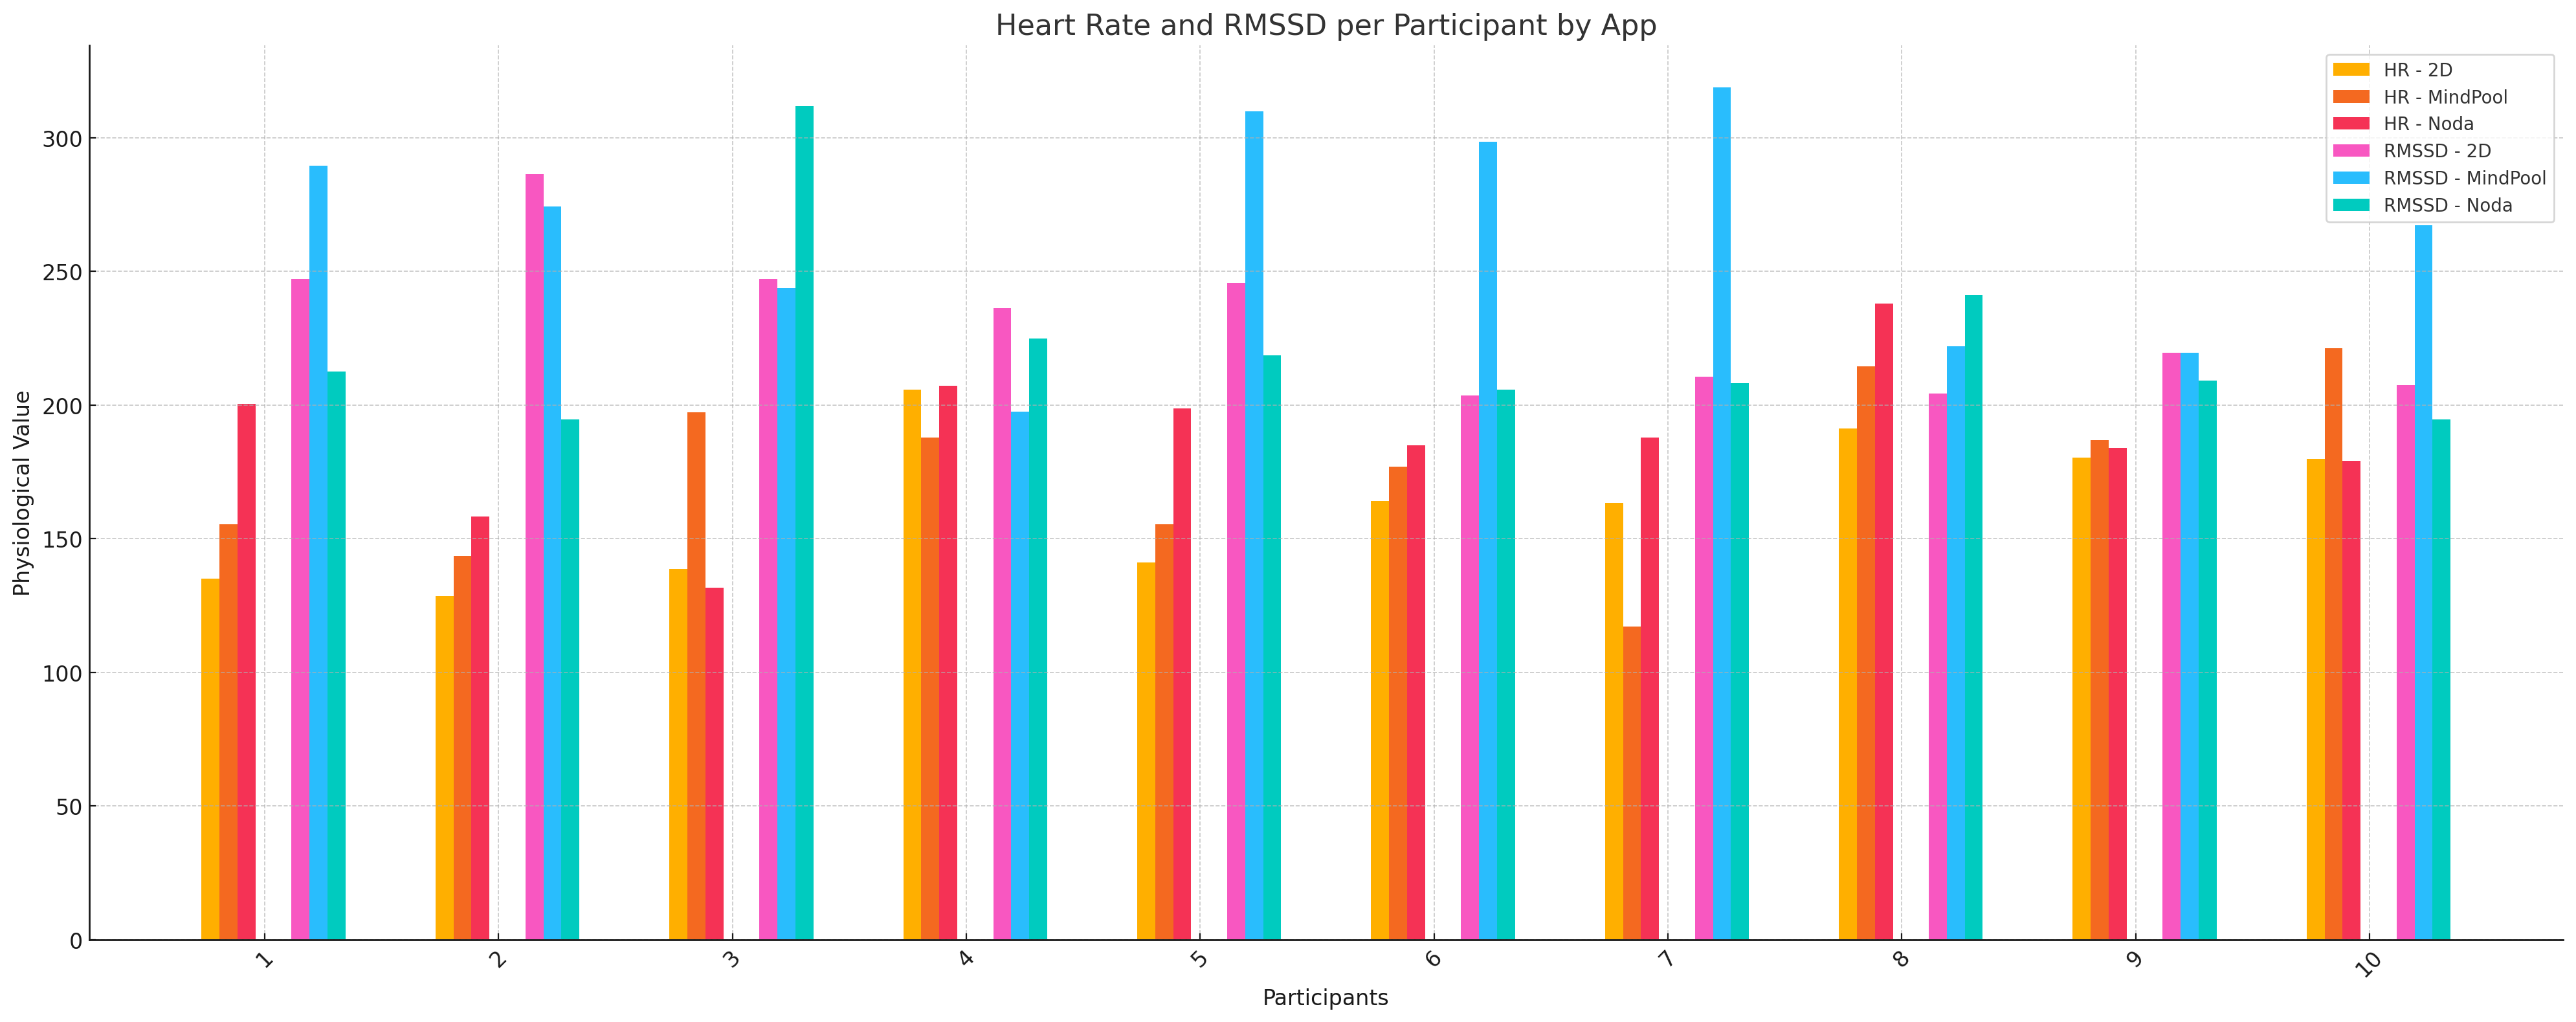
\includegraphics[width=1\textwidth]{fig/physiological/HR_RMSSD_per_Part_by_App.png}
\caption{Heart Rate and RMSSD per Participant by App.}
\label{fig:rmssd_boxplot}
\end{figure}


% A comparative analysis of physiological signals—specifically \textit{heart rate (HR)} and \textit{root mean square of successive differences (RMSSD)}—was conducted to infer participant stress and autonomic nervous system activity across the three application environments: Xmind (2D), Noda (VR), and (MindPool custom VR).

Overall, MindPool demonstrated competitive physiological profiles compared to both Noda and the Xmind 2D App. In terms of heart rate, which tends to increase under stress or elevated cognitive demand \citep{andreassi2000psychophysiology,solhjoo2019heart,ward2003physiological,wilson2001psychophysiological}, most of the participants (P1, P2, P4, P5, P6, P7) showed lower average BPM while using MindPool compared to Noda, suggesting reduced stress or more efficient cognitive engagement. This pattern was particularly notable in participants who exhibited elevated heart rates in the Noda condition but moderate levels in MindPool. However, the Xmind 2D app participants portrayed the lowest heart rates overall which was expected due to it not being as engaging as the VR counterparts.

Complementing this, RMSSD - a time-domain measure of heart rate variability linked to parasympathetic nervous system activity - was often higher in MindPool for several participants (P1, P2, P3, p4, p5, p10). Since higher RMSSD generally reflects better physiological regulation and lower mental strain \citep{Mehler2012,Fine2022}, these results may indicate that MindPool facilitated a calmer and more cognitively balanced interaction for a subset of users.

However, inter-participant variability was substantial, with no single app universally outperforming across all users. For instance, while MindPool led to favorable results in some cases, other participants (e.g., P3, P4) showed either comparable or slightly elevated stress indicators relative to Xmind or Noda.
% , highlighting the \textit{importance of individual differences in spatial navigation familiarity, VR tolerance, or cognitive style}.

In summary, although not universally dominant, MindPool appears to offer physiological advantages for many participants manifesting as reduced heart rate or increased HRV—suggesting potential improvements in user comfort and cognitive manageability over existing VR or 2D solutions.

It is also noteworthy that the average heart rate values across all participants were consistently reported above 120 BPM by the AcqKnowledge software during HRV analysis. This contrasts with raw signal observations, where heart rate readings generally remained closer to 100 BPM for most of the session duration. This discrepancy may be attributed to differences in how AcqKnowledge computes heart rate averages during HRV analysis, potentially involving preprocessing or epoch-level aggregation that differs from raw signal inspection. As such, while relative comparisons between application conditions remain valid, absolute heart rate values should be interpreted with caution.

\subsection{Descriptive Trends}

Descriptive statistics (see Table~\ref{tab:descriptive_statistics_of_physiological}) revealed that participants using the Noda app exhibited the highest mean heart rate (indicating higher physiological arousal or engagement), followed by MindPool and then XMind. In contrast, RMSSD values were relatively similar across conditions, suggesting comparable levels of autonomic balance and stress response. Task completion times showed substantial differences: participants completed the mind mapping task fastest in XMind, followed by MindPool, and slowest in Noda.

\begin{table}[ht]
\centering
\caption{Descriptive statistics of physiological measures by app condition (Mean ± SD)}
\begin{tabular}{|c|c|c|c|}
\hline
\textbf{App} & \textbf{Mean Heart Rate (BPM)} & \textbf{RMSSD (ms)} & \textbf{Total Task Time (min)} \\
\hline
2D (XMind)   & 149.73 ± 28.77 & 256.32 ± 20.61 & 7.65 ± 0.64 \\
MindPool     & 167.44 ± 21.51 & 262.53 ± 44.58 & 13.85 ± 1.67 \\
Noda         & 179.16 ± 30.82 & 232.87 ± 41.33 & 17.64 ± 2.80 \\
\hline
\end{tabular}
\label{tab:descriptive_statistics_of_physiological}
\end{table}

Boxplot visualizations provide additional insight into these patterns. The task time boxplot (Figure~\ref{fig:time_boxplot}) shows a tightly clustered distribution for XMind, while both VR conditions required more time, with Noda exhibiting the widest spread and longest durations. The heart rate boxplot (Figure~\ref{fig:hr_boxplot}) illustrates that participants in the Noda condition experienced elevated physiological arousal, whereas MindPool elicited moderate heart rate values and XMind the lowest. Finally, the RMSSD boxplot (Figure~\ref{fig:rmssd_boxplot}) shows a trend toward higher HRV values in the MindPool condition compared to 2D and Noda. While this visual pattern suggests a potential difference in autonomic stress regulation, the variation needs to be verified whether they are statistically significant according to the Friedman test for interpretation.

Taken together, these trends suggest that MindPool—while still more demanding than XMind—may offer an improved and more efficient experience than Noda, as reflected in reduced heart rate and task duration.


\begin{figure}[H]
\centering
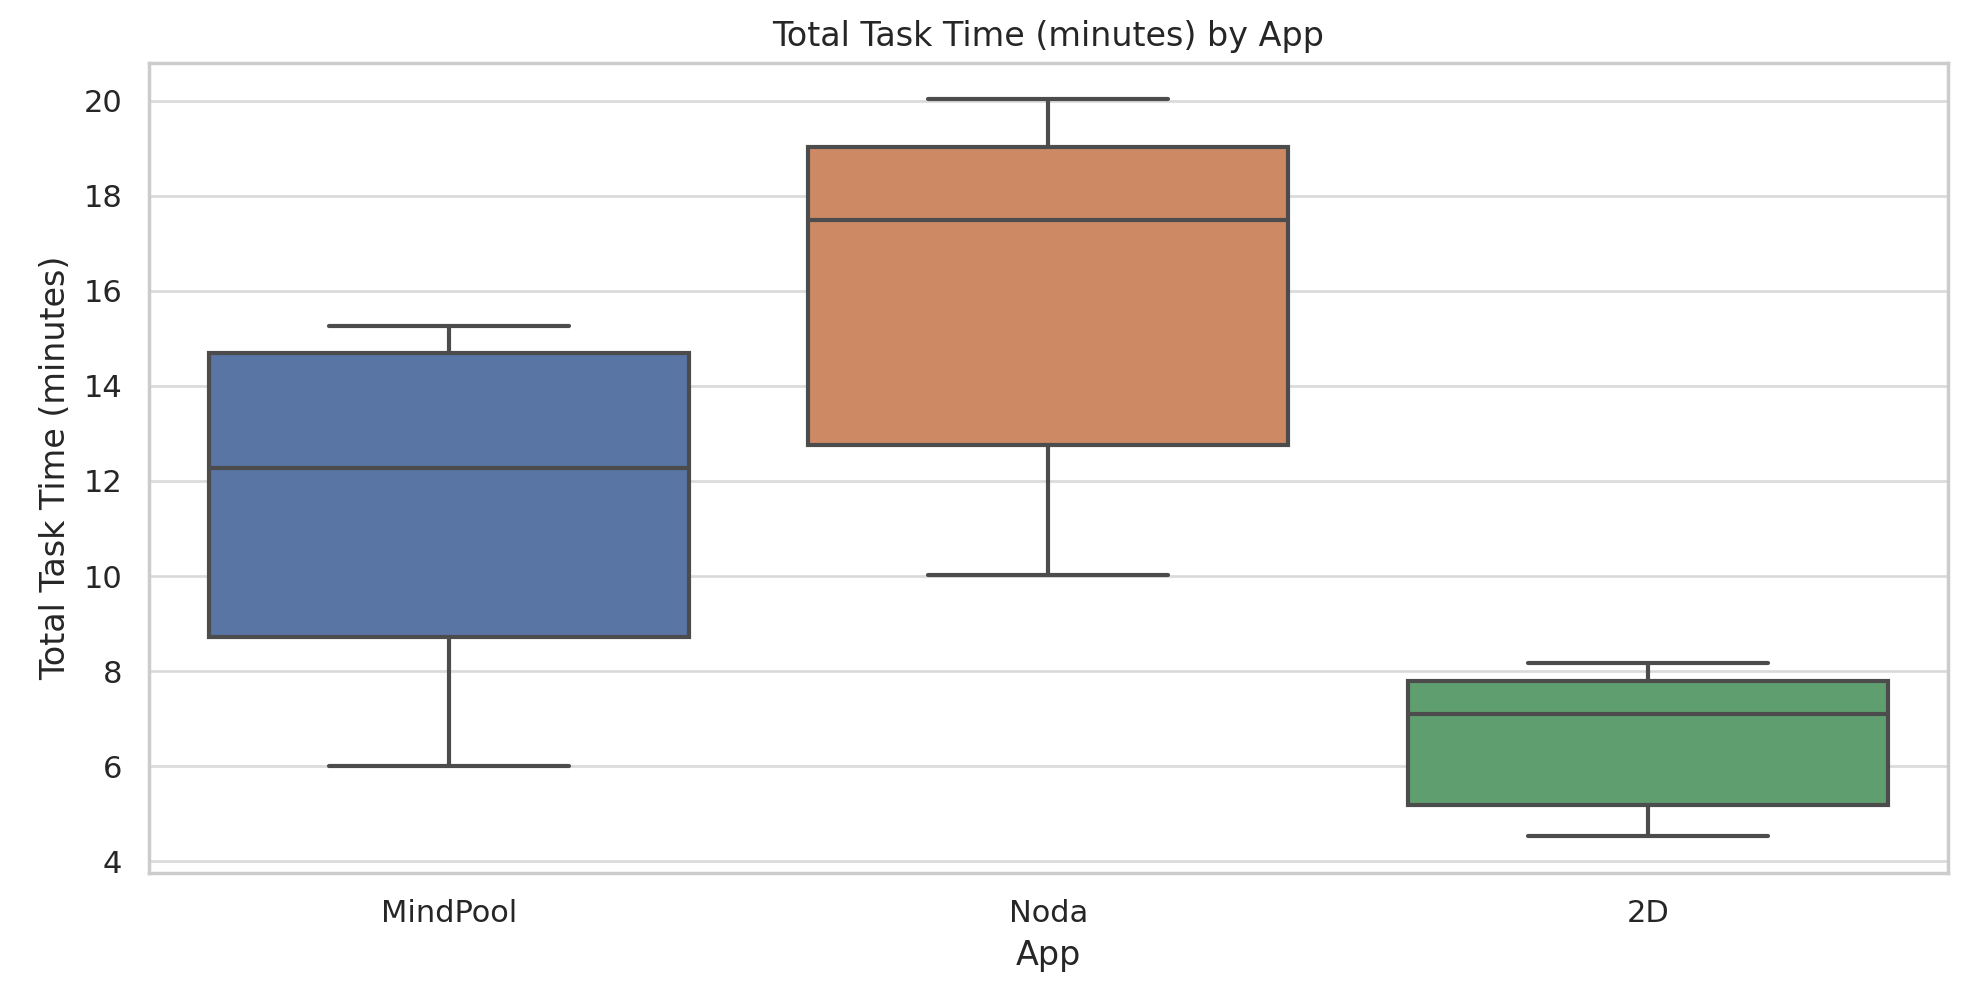
\includegraphics[width=0.8\textwidth]{fig/physiological/TaskTime_by_App.png}
\caption{Total Task Time by App.}
\label{fig:time_boxplot}
\end{figure}

\begin{figure}[H]
\centering
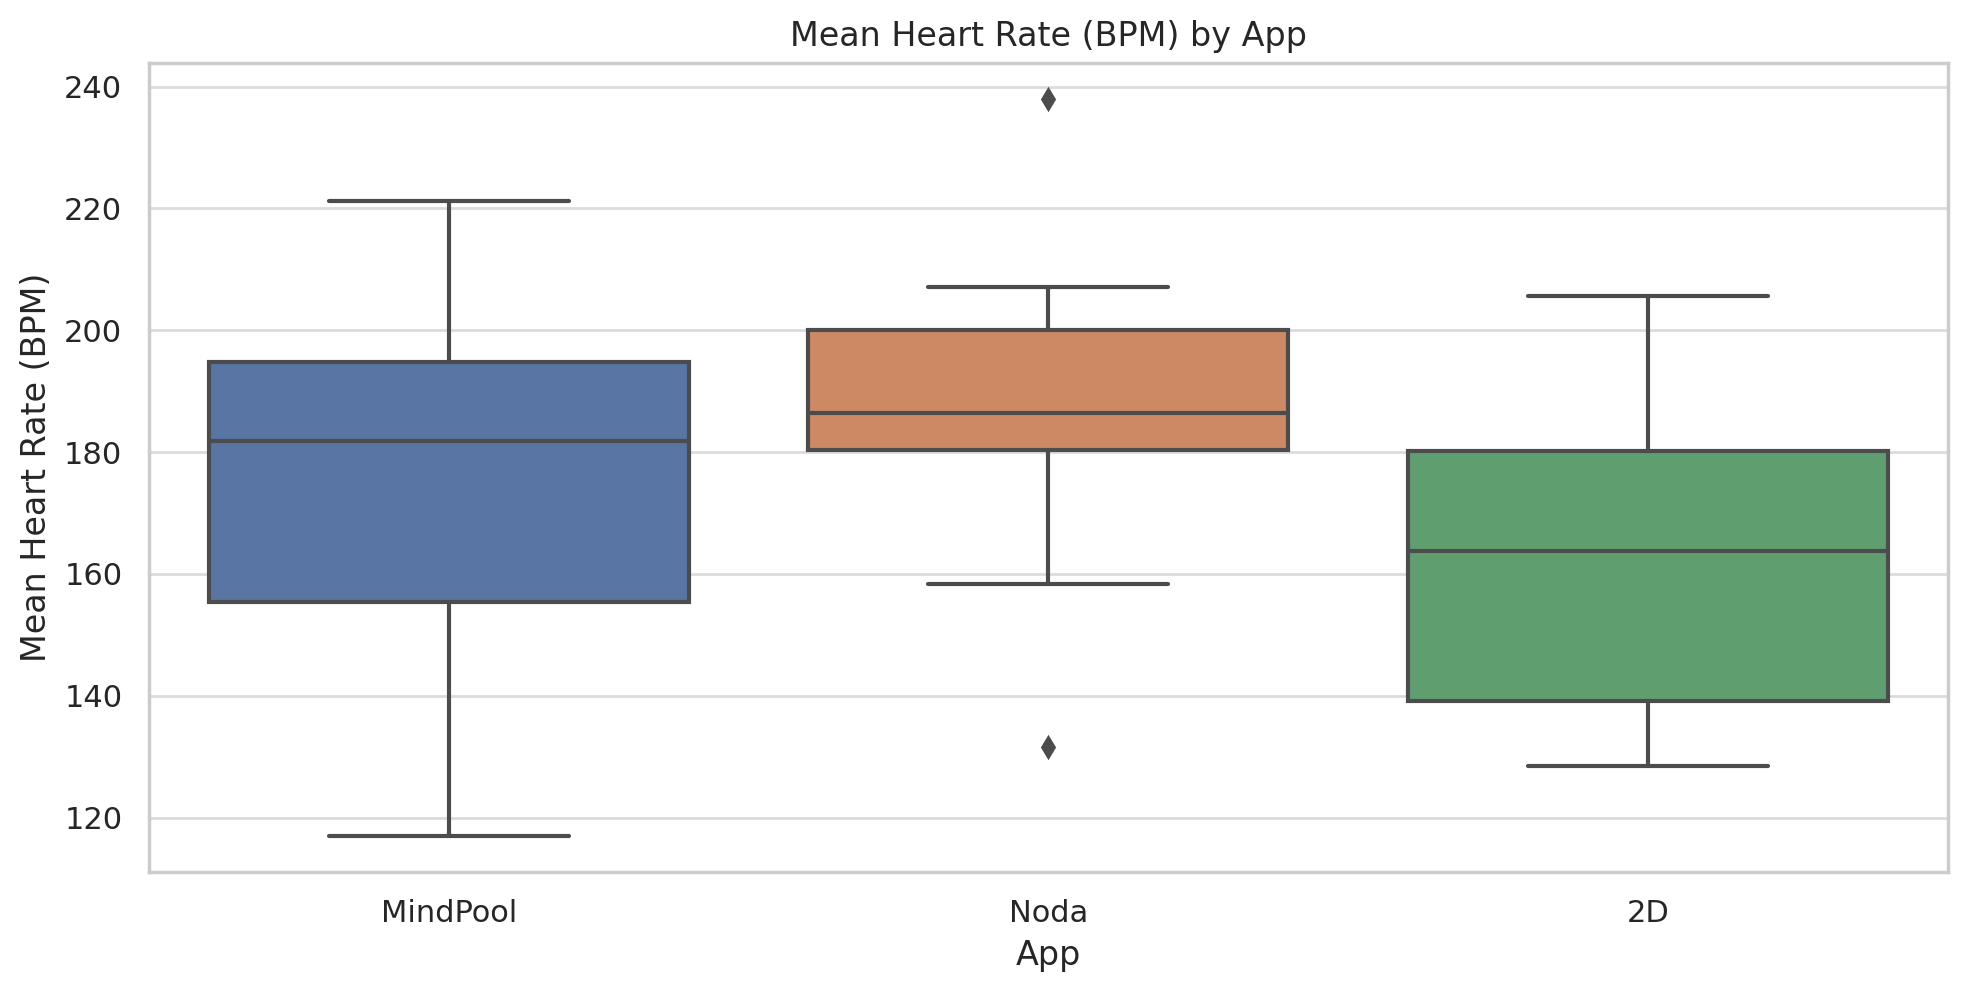
\includegraphics[width=0.8\textwidth]{fig/physiological/Mean_HR_by_App.png}
\caption{Mean Heart Rate by App.}
\label{fig:hr_boxplot}
\end{figure}

\begin{figure}[H]
\centering
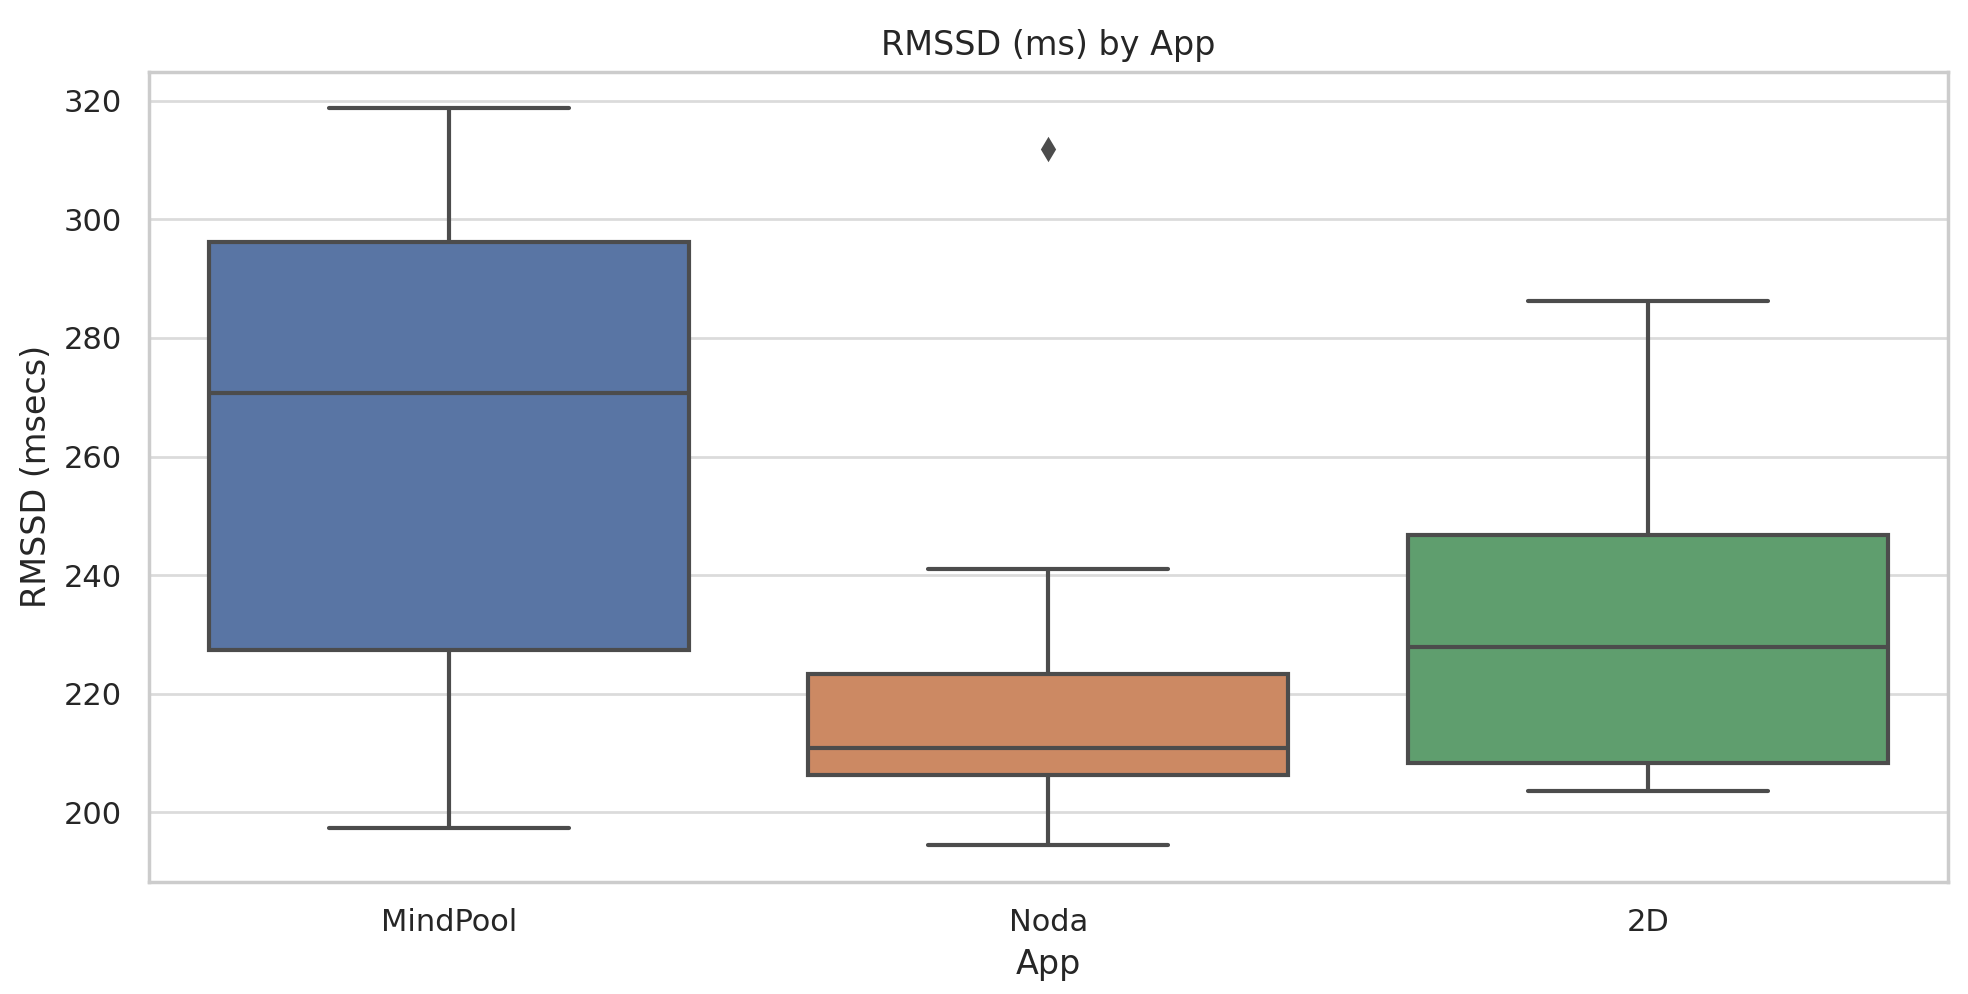
\includegraphics[width=0.8\textwidth]{fig/physiological/RMSSD_by_App.png}
\caption{RMSSD by App.}
\label{fig:rmssd_boxplot}
\end{figure}





\subsection{Statistical Testing}

To evaluate the significance of physiological differences across app conditions, non-parametric Friedman tests were conducted for each metric and is shown in Table~\ref{tab:friedman_phy}. 

\begin{table}[h!]
\centering
\caption{Friedman Test Results}
\begin{tabular}{|l|c|c|c|}
\hline
\textbf{Category} & \textbf{Friedman Statistic} & \textbf{p-value} & \textbf{Significant $(p < .05)$} \\
\hline
Total Task Time & 20.00 & 0.001 & Yes \\
Mean Heart Rate & 6.20 & 0.045 & Yes \\
RMSSD & 2.60 & 0.273 & No \\
\hline
\end{tabular}
\label{tab:friedman_phy}
\end{table}


Results indicated:

    A significant difference in mean heart rate across conditions $(\chi^2(2) = 6.20, p = .045)$.

    No significant difference in RMSSD values $(\chi^2(2) = 2.60, p = .273)$.

    A highly significant difference in task completion times $(\chi^2(2) = 20.00, p < .001)$.

\begin{table}[h!]
\centering
\caption{Wilcoxon Signed-Rank Test Results}
\begin{tabular}{|l|l|c|c|}
\hline
\textbf{Category} & \textbf{Comparison} & \textbf{Wilcoxon Statistic} & \textbf{p-value} \\
\hline
Mean Heart Rate & XMind vs Noda & 5.0 & 0.0195 \\
Total Task Time & XMind vs Noda & 0.0 & 0.002 \\
Total Task Time & XMind vs MindPool & 0.0 & 0.002 \\
Total Task Time & Noda vs MindPool & 0.0 & 0.002 \\
\hline
\end{tabular}
\label{tab:wilcoxon_phy}
\end{table}


Follow-up Wilcoxon signed-rank tests (see Table~\ref{tab:wilcoxon_phy}) pinpointed where these differences occurred:

    Heart Rate: Significant increase from XMind to Noda $(p = .0195)$; no significant differences between MindPool and either of the other two.

    Task Time: All pairwise comparisons were significant $(p = .002)$, with XMind requiring the least time, followed by MindPool, then Noda.

\subsection{Interpretation}

The significantly higher heart rate in the Noda condition may reflect greater physiological arousal or cognitive strain compared to the 2D app. However, the lack of significant differences in RMSSD suggests that stress-related autonomic regulation remained similar across conditions. The markedly longer task times in VR, especially in Noda, indicate usability challenges or increased cognitive demand. Notably, the custom-built MindPool app demonstrated improved task efficiency over Noda, aligning with its design goals for enhanced usability.

These physiological findings reinforce the questionnaire results and underscore the potential of HRV and heart rate metrics as complementary indicators of user experience in immersive technologies.




\section{Qualitative Insights}

At the conclusion of the study, participants completed a qualitative interview consisting of six open-ended questions. Their responses are summarized below by question category.

\subsection{App Enjoyment Ranking (Motivation)}
When asked to rank the apps by overall enjoyment:

\begin{itemize}
    \item 9 participants ranked MindPool as the most enjoyable app, followed by Noda, and then XMind.
    \item 1 participant ranked Noda as most enjoyable, followed by MindPool, and then XMind.
\end{itemize}

Participants cited MindPool's immersive environments, multiple browser functionality, AI features, and more natural interaction design as factors contributing to greater enjoyment.

\subsection{App Ease of Use}
In ranking the apps for ease of use:

\begin{itemize}
    \item 3 participants ranked MindPool first, followed by XMind, then Noda.
    \item 6 participants ranked XMind first, followed by MindPool, then Noda.
    \item 1 participants ranked XMind first, followed by Noda, then MindPool.
\end{itemize}

Ease of use perceptions reflected familiarity with 2D systems and appreciation for MindPool’s control labeling and improved UI compared to Noda.

\subsection{Ease of Getting Started (Tutorial Experience)}
Participants unanimously reported that MindPool was the easiest app to get started with, highlighting:
\begin{itemize}
    \item Clear visibility of the tutorial video player.
    \item Controller-mapped functionality labels.
    \item A comprehensive tutorial that covered all essential features.
\end{itemize}
In contrast, participants noted that XMind, had an overwhelming and segmented tutorial that was harder to navigate. Noda's progressive tutorial system was criticized for requiring task-by-task completion without having the the flexibility to revisit previous tutorial portions and failing to cover some important features (e.g., alternate ways to delete nodes).

\subsection{Perceived Cognitive Load During Thought Organization}

In response to the question, "In which app did you feel it was easiest to organize your thoughts without feeling overwhelmed?"—which was aimed at assessing perceived cognitive load—all 10 participants ranked the apps in the same order as their earlier usability ratings:
XMind $>$ MindPool $>$ Noda.
Participants cited XMind’s familiar interface and streamlined 2D layout as reasons it made thought organization feel less cognitively demanding.

\subsection{Long-Term Use Preference}

When asked which app they would prefer for regular, long-term mind mapping, all 10 participants again indicated a preference for:
XMind $>$ MindPool $>$ Noda.
They explained that for frequent use, XMind’s simplicity, speed, and familiarity made it the most appealing.

However, when specifically asked whether their preference would change for much larger and more complex mind maps, participants shifted their rankings to:
MindPool $>$ XMind $>$ Noda.
They noted that MindPool’s immersive space, scalable layout, and AI support made it better suited for handling expansive, multi-branching maps.

Additionally, 3 participants expressed a desire for a hybrid solution—preferring to start in XMind and transition to MindPool only when the mind map became too large for a 2D layout to remain manageable.


\subsection{Impressions of AI Features (AI Note and AI Avatar)}
All participants reported finding the AI features in MindPool useful and enjoyable. Common feedback included:
\begin{itemize}
    \item The AI Avatar interaction (voice-based) felt more natural, personal, and immersive compared to typing.
    \item AI-assisted responses helped speed up cognitive tasks and enhance engagement.
    \item Participants emphasized that AI should supplement, not replace the keyboard — preferring to have both modalities available.
\end{itemize}
\subsection{Likes, Dislikes, and Suggested Improvements}
Participants offered detailed feedback regarding app features:
\subsubsection{MindPool}
Strengths:
\begin{itemize}
    \item Better and more intuitive keyboard (leveraging Meta’s default).
    \item Reliable and clearer speech-to-text performance.
    \item Multiple browser spawning and resizing, resembling desktop experiences.
    \item Cleaner, simpler menu that followed user head movement.
    \item Ability to manipulate notes and browsers from a distance.
    \item Higher-quality environment options and more variety.
    \item Tutorial video player praised for being easy to access and covering all core features.
\end{itemize}
Areas for Improvement:
\begin{itemize}
    \item Some participants wished for a toggle to make the floating menu stationary if desired.
    \item A few commented that they wished the UI was even more streamlined aesthetically only if it does not come at the cost of ease of use.
    \item An auto-arrange feature was suggested by several participants, allowing users to automatically distribute elements (notes, browsers, AI avatar) around the scene for better visibility as maps grew larger since at times some of the elements were hidden behind other elements.
    \item In-app volume control for background music would be a helpful addition.
\end{itemize}
\subsubsection{Noda}
  Strengths:
  \begin{itemize}
    \item Participants praised the ease of creating a connection between nodes over MindPool
    \item One participant liked the immersive depth of the retro environment provided by Noda 
    
    \end{itemize}
Criticisms:
\begin{itemize}
    \item Participants universally disliked the trigger control behavior: accidental node creation when trying to select nodes.
    \item The keyboard UI was considered not user friendly (unclear backspace button, missing dollar symbol, auto-reverting number panel).
    \item Speech-to-text was reported to be inaccurate at times and lacking clear indicators for listening status especially while inserting prices in notes.
    \item Browser elements could not be resized, leading to information being partially cut off.
    \item Object manipulation required close physical proximity. Some participants preferred having the option to being able to manipulate over a distance.
    \item Participants preferred MindPool’s controller orientation-based pointing system over Noda’s static raycasting.
    \item Many participants liked Noda’s minimalistic visual design, but acknowledged that it came at the cost of usability.
\end{itemize}



\newpage

\chapter{Discussion}

\section{Cross-Modal Comparison: Physiological, Questionnaire, and Qualitative Insights}

The integration of physiological metrics, standardized questionnaire data, and qualitative participant feedback enables a triangulated interpretation of user experience across the three app conditions—XMind (2D), Noda (VR), and MindPool (custom VR). Each modality contributes a unique perspective on cognitive load, usability, and motivation, but taken together, they offer a coherent and mutually reinforcing narrative.

\subsection{Cognitive Load}

\subsubsection{Questionnaire Data (RTLX):}
 XMind received the lowest cognitive load ratings, followed by MindPool, and then Noda, which scored highest. The difference between XMind and Noda was statistically significant, indicating that participants perceived Noda to be considerably more mentally and physically demanding. MindPool’s intermediate scores suggest it successfully balanced immersion with efficiency.

\subsubsection{Physiological Data (Heart Rate & RMSSD):}
 Heart rate data supports these findings—Noda consistently induced the highest BPM values, while XMind maintained the lowest. MindPool again fell in between but trended closer to XMind for many participants. RMSSD, an HRV indicator associated with stress resilience, showed no significant difference overall, yet several participants had higher RMSSD in MindPool compared to Noda, reinforcing the idea that MindPool mitigates physiological stress more effectively.

\subsubsection{Qualitative Data:}
 Participants noted that Noda felt overwhelming due to control design and interaction inconsistencies. Conversely, they found MindPool’s tutorial, UI clarity, and flexible input options contributed to smoother interactions and less confusion. XMind’s familiarity also reduced cognitive overhead but lacked immersive engagement.

Taken together, these results converge to suggest that MindPool represents a viable middle ground—reducing VR-associated strain while introducing motivational benefits absent in traditional 2D systems.

\subsection{Usability}

\subsubsection{Questionnaire Data (SUS):}
 MindPool was rated highest in usability, significantly outperforming Noda and being comparable to XMind. Noda scored lowest, with participants highlighting frustrations related to the interface and control logic.

\subsubsection{Physiological Data (Task Time):}
 Task completion time serves as an indirect usability measure. XMind was the fastest, followed by MindPool, and then Noda. The significantly longer times required in Noda suggest usability barriers and learning curve inefficiencies. MindPool’s reduced task time, despite being in VR, validates its improved interface design.

\subsubsection{Qualitative Data:}
 Participants praised MindPool’s keyboard, browser spawning, and note manipulation features, specifically noting how these improvements addressed pain points encountered in Noda. While XMind benefited from its 2D simplicity, it lacked the rich interaction potential offered by VR environments. Noda’s usability was further criticized for issues like imprecise speech-to-text and non-intuitive controls.

This multimodal convergence supports the conclusion that MindPool’s design enhancements yield real usability improvements in immersive settings, bringing VR interaction quality closer to that of traditional platforms.

\subsection{Motivation and Engagement}

\subsubsection{Questionnaire Data (IMI):}
 MindPool achieved the highest scores across all motivation subscales, including interest/enjoyment, relatedness, and perceived competence. These were significantly higher than both Noda and XMind. Noda scored lowest in several motivation subcomponents.

\subsubsection{Physiological Data (Heart Rate):}
 Although high heart rate is not a direct measure of motivation, elevated BPM values in Noda—paired with low IMI scores—may indicate stress or discomfort rather than engagement. In contrast, MindPool maintained more moderate heart rates despite being immersive, suggesting a healthier engagement profile.

\subsubsection{Qualitative Data:}
 Participants overwhelmingly preferred MindPool for overall enjoyment and AI features. The AI avatar and note assistant were frequently mentioned as enjoyable, supportive tools that made the app feel more interactive and intelligent. This aligns with higher IMI scores, suggesting that immersive features can significantly boost intrinsic motivation when implemented effectively.

These cross-modal insights indicate that while VR does not inherently guarantee higher motivation, thoughtful design choices like those in MindPool can successfully leverage immersion to increase engagement.

\subsection{Summary}

MindPool consistently outperformed Noda and approached or surpassed XMind in various metrics, demonstrating that iterative improvements can close the gap between VR and traditional UIs in usability, reduce VR-induced cognitive load, and elevate user motivation. Importantly, the alignment between physiological, questionnaire-based, and qualitative measures strengthens the validity of these conclusions, supporting the core dissertation that a mixed-method evaluation strategy reveals deeper insights than any single modality alone.


% \section{App-Specific Observations}

% \section{Challenges}

% \subsection{Limitations}

% While the findings of this study provide valuable insights into the comparative user experience of 2D and XR mind mapping applications, several limitations should be acknowledged:

% \begin{enumerate}
%     \item \textbf{Small Sample Size:} The study involved only 10 participants, which limits the statistical power of inferential tests and the generalizability of results. The small sample size increases susceptibility to individual differences and may obscure subtle effects, particularly in analytical values like mean heart rate and RMSSD obtained from physiological data.
    
%     \item \textbf{Limited Demographic Diversity:} All participants were recruited via convenience sampling, primarily from similar academic groups (Bachelor's and Master's) and age groups (20-25). As such, the results may not represent the broader population, especially users with less technological proficiency or different cognitive profiles.

%     \item \textbf{Controlled Task Design:} While a uniform restaurant comparison task ensured consistency across conditions and a reasonable total study time per participant to be around one hour, it may not encompass the full spectrum of cognitive and creative demands typical of real-world mind mapping use, suggesting opportunities for broader exploration in future studies

%     \item \textbf{Learning Effects and Familiarity Bias:} Despite counterbalancing task order across participants, some learning effects may still have occurred. Additionally, users' familiarity with 2D interfaces likely favored XMind in usability and task speed, potentially disadvantaging the VR apps.

%     \item \textbf{Physiological Signal Interpretation:} Physiological metrics such as heart rate and RMSSD are influenced by numerous internal and external factors (e.g., movement, breathing patterns, baseline fitness) beyond cognitive load or stress. Furthermore, discrepancies between raw and HRV-processed heart rate values in AcqKnowledge raise concerns about the reliability of absolute measurements, though relative trends remained interpretable.

%     \item \textbf{VR Comfort and Tolerance Variability:} Some participants may have experienced motion sickness or VR fatigue, which could have affected both subjective and physiological responses. These individual differences were not explicitly controlled for or measured.

%     \item \textbf{Prototype vs. Production Quality:} MindPool was a custom-built prototype. While it aimed to improve upon Noda, it may have benefited from novelty effects or researcher enthusiasm. Conversely, its prototype status may have introduced rough edges not present in commercially polished apps, influencing user impressions.

%     \item \textbf{Qualitative Data Interpretation:} Although qualitative feedback enriched the findings, participant comments were not systematically coded or analyzed using rigorous qualitative analysis frameworks, limiting the depth and reproducibility of this component.
% \end{enumerate}



% \section{Future Research Directions}


\section{Limitations and Future Work}

While this study provides valuable insights into the comparative experience of 2D and XR mind mapping applications, several limitations constrain the scope and generalizability of the findings. These limitations also offer clear directions for future research:

\begin{itemize}
    \item \textbf{Small Sample Size:} The study involved only 10 participants, which limits the statistical power of inferential tests and the generalizability of results. The small sample size increases susceptibility to individual differences and may obscure subtle effects, particularly in analytical values like mean heart rate and RMSSD obtained from physiological data. Future studies should recruit a larger and more diverse participant pool to enable more robust statistical conclusions and generalizability across user types.

    \item \textbf{Demographic Homogeneity:} Most participants were of similar academic background (Bachelor's and Master's) and age range (20--25). Future work should include participants from a broader demographic spectrum—such as different age groups, educational levels, and levels of technological familiarity—to better reflect real-world user diversity.

    \item \textbf{Controlled Task Constraints:} While a uniform task enabled consistency in measurement, it may not capture the full complexity of mind mapping use in authentic scenarios. Subsequent research should investigate more open-ended or domain-specific tasks (e.g., brainstorming, academic planning) to assess real-world applicability and flexibility.

    \item \textbf{Learning Effects and Familiarity Bias:} Although counterbalancing was used, participants' prior familiarity with 2D interfaces may have skewed usability and performance ratings. Future research could include longer pre-study VR training sessions or longitudinal designs to better assess adaptation effects over time.

    \item \textbf{Physiological Signal Complexity:} Heart rate and HRV metrics can be affected by a range of external variables (e.g., posture, motion, respiration). To improve physiological signal reliability, future studies should consider multi-sensor setups (e.g., combining EEG or eye tracking), baseline normalization techniques, and additional preprocessing steps to isolate cognitive load-specific responses.

    \item \textbf{VR Comfort and Tolerance Differences:} Variability in VR tolerance (e.g., susceptibility to motion sickness) was not measured due to the stationary nature and short duration of the tasks. Future work could include standardized VR comfort questionnaires or pre-screening to account for such variability and better contextualize participant responses.

    \item \textbf{Prototype Design Constraints:} MindPool, as a research prototype, may have introduced novelty effects or imperfections not found in commercial applications. Future iterations could aim for higher fidelity and extended user testing in production-like environments to validate findings under more realistic conditions.

    \item \textbf{Qualitative Analysis Depth:} While open-ended responses enriched the findings, they were not formally coded or thematically analyzed. Future studies could employ rigorous qualitative methodologies (e.g., thematic coding, inter-rater reliability) to extract deeper insights from user feedback and triangulate them more formally with quantitative data.

    \item \textbf{Heart Rate Data Discrepancy:} A key limitation observed during post-analysis was that average pulse rate values appeared much higher than expected across all applications and participants. While the AcqKnowledge software displayed acceptable values during live recording, further inspection revealed that pulse rate data derived from PPG was filtered during display to cap any value above 120 bpm. However, in the recorded data used for analysis, actual values exceeding 120 bpm were retained, skewing average heart rate calculations. This discrepancy, possibly compounded by limitations in the Biopac ring’s accuracy, highlights the need for future studies to replicate the analysis using alternative physiological sensors or devices to validate the findings. Due to time constraints, the current study includes the originally calculated average heart rate values, but an updated analysis with capped values will be published in future work.

    \item \textbf{Stress Induction Limitations in Task Design:} The chosen task—creating a mind map—may not have elicited sufficiently high levels of cognitive or emotional stress to clearly differentiate physiological responses across conditions. While the task enabled controlled comparison, it may lack the intensity required to observe pronounced stress-induced differences using tools like the Biopac ring. Future research could incorporate more stress-inducing tasks (e.g., timed problem-solving, driving simulators, or VR horror environments) to explore how varying levels of cognitive or emotional load influence usability perceptions and physiological responses between 2D and XR mind mapping applications.
\end{itemize}

Addressing these limitations in future work will strengthen the validity and applicability of results, offering a more comprehensive understanding of how XR and 2D mind mapping tools impact user experience across cognitive, emotional, and physiological dimensions.



\newpage

\chapter{Conclusion}








\section{Summary of Findings}

This study set out to compare the cognitive load, usability, and intrinsic motivation associated with 2D and XR mind mapping applications using a combination of physiological signal analysis and traditional questionnaire-based evaluation. The findings demonstrated that XMind (2D) was the least cognitively demanding, while MindPool—an iteratively improved VR application—emerged as the most engaging and usable. Noda, the baseline VR app, consistently underperformed across most metrics.

From a physiological perspective, heart rate and HRV data provided objective support for participants' subjective impressions. Higher heart rates and longer task times were observed in Noda, indicating higher cognitive strain and lower usability. In contrast, MindPool showed a more balanced physiological response, suggesting a successful design balance between immersion and efficiency.

Traditional questionnaires (RTLX, IMI, SUS) reinforced these patterns: XMind yielded the lowest cognitive load scores, while MindPool achieved the highest ratings for usability and motivation. Qualitative feedback further corroborated these results, with participants overwhelmingly favoring MindPool for its AI features, intuitive UI, and immersive yet manageable environment.

Collectively, these findings affirm that XR environments, when thoughtfully designed, can provide not only engaging but also efficient and usable alternatives to traditional 2D tools.

\section{Contributions Revisited}

This thesis makes two primary contributions to the field of human-computer interaction and educational technology:

\subsection{Physiological Signal Integration in XR Usability Research} This study is among the first to incorporate physiological data—specifically heart rate and HRV derived from PPG signals—into the comparative evaluation of 2D and XR mind mapping applications. By coupling objective physiological metrics with established subjective questionnaires (RTLX, IMI, SUS), this research introduces a novel, multimodal methodology for assessing cognitive load, stress, and engagement in immersive systems.

\subsection{Iterative Development of an AI-Enhanced XR Mind Mapping App}
 The custom-built VR application, MindPool, represents a substantial advancement over existing tools like Noda. MindPool’s improvements include a better-designed keyboard, multiple browser support, expandable notes, and the introduction of AI-enhanced features such as a voice-interactive AI avatar and content-aware AI note assistant. These additions significantly improved usability and motivation without increasing cognitive strain, as demonstrated by both subjective and physiological data.

Together, these contributions not only advance methodological approaches in XR research but also provide a practical design case study illustrating how iterative improvements and AI integration can meaningfully enhance user experience in immersive environments.

\section{Final Thoughts on XR Mind Mapping’s Potential}

The results of this study offer evidence that XR has the potential to revolutionize digital knowledge work, especially in areas like brainstorming, concept mapping, and structured note-taking. While traditional 2D tools remain valuable for their simplicity and efficiency, XR tools—if well-designed—can provide richer, more engaging experiences without necessarily increasing user burden.

MindPool exemplifies how careful attention to usability, feature integration, and user feedback can transform XR from a novelty into a viable productivity platform. With the added benefit of AI augmentation, XR mind mapping applications may soon evolve into intelligent, immersive cognitive companions that adapt to users’ workflows and enhance both creative and analytical thinking.

As XR hardware becomes more accessible and AI continues to evolve, the fusion of these technologies promises to reshape not only how we visualize ideas but also how we think, learn, and collaborate. This study serves as a foundation for future research and development in this promising intersection of immersive technology and cognitive tools.

\section{Software Availability}

MindPool, the XR mind mapping app developed for this study, is scheduled for release on the Meta Quest Store. Access to the source code may be requested by contacting the author.


% \begin{thebibliography}{99}
% \addcontentsline{toc}{chapter}{{Bibiliography}}

% \bibitem{ber} F. Bermudez, A. Medina, A. Rosin, E. Scott. {\it Are Stupid Dice Necessary?}, The College Mathematics Journal, Vol. 44, No. 4, September 2013.

% \bibitem{gal} J. Gallian, {\it Contemporary Abstract Algebra}, Houghton Mifflin Company, 2008.

% \bibitem{gas} W. Gasarch, C. Kruskal, {\it When Can One Load a Set of Dice so That the Sum Is Uniformly Distributed?}, Mathematics Magazine 72, 1999.

% \end{thebibliography}


\SuppChap  % So the ToC doesn't prepend "Chapter" to your bibliography
\addcontentsline{toc}{chapter}{Bibliography}
\bibliographystyle{apalike}  % You can change this to plain, IEEEtran, etc.
\bibliography{references}    % Use your actual .bib file name, no extension

% \SuppChap % Disable chapter prefixes in ToC

% \chapter*{Bibliography}
% \addcontentsline{toc}{chapter}{Bibliography}
% \bibliographystyle{plain}
% \bibliography{myrefs}


\SuppChap  % So the ToC doesn't prepend "Chapter" to your bibliography

\chapter*{Appendix}
\addcontentsline{toc}{chapter}{Appendix}

% \AddAppendix % Updates the style for the Table of Contents
% \begin{appendices}
 % \chapter{Appendix}


\begin{table}
\centering
\caption{HRV Data for 2D App}
\label{tab:2d_hrv}
\begin{tabular}{|c|c|c|c|}
 \hline
 Participant & Total Task Time (mins) & Mean Heart Rate (BPM) & RMSSD (msecs) \\
 \hline
 1  & 8.16 & 135.11 & 247.06 \\
 2  & 7.62 & 128.43 & 286.30 \\
 3  & 8.01 & 138.57 & 247.21 \\
 4  & 6.25 & 205.70 & 236.23 \\
 5  & 7.60 & 141.11 & 245.76 \\
 6  & 6.57 & 164.07 & 203.59 \\
 7  & 7.86 & 163.33 & 210.68 \\
 8  & 4.82 & 191.16 & 204.41 \\
 9  & 4.67 & 180.25 & 219.60 \\
 10 & 4.54 & 179.86 & 207.48 \\
 \hline
\end{tabular}
\end{table}





\begin{table}
\centering
\caption{HRV Data for MindPool App}
\label{tab:mindpool_hrv}
\begin{tabular}{|c|c|c|c|}
 \hline
 Participant & Total Task Time (mins) & Mean Heart Rate (BPM) & RMSSD (msecs) \\
 \hline
 1  & 15.25 & 155.32 & 289.53 \\
 2  & 14.89 & 143.54 & 274.16 \\
 3  & 10.02 & 197.20 & 243.79 \\
 4  & 14.09 & 187.75 & 197.41 \\
 5  & 15.00 & 155.38 & 309.75 \\
 6  & 11.00 & 176.86 & 298.39 \\
 7  &  8.28 & 117.02 & 318.70 \\
 8  & 13.54 & 214.53 & 221.87 \\
 9  &  6.00 & 186.86 & 219.54 \\
 10 &  6.62 & 221.21 & 267.15 \\
 \hline
\end{tabular}
\end{table}


\begin{table}
\centering
\caption{HRV Data for Noda App}
\label{tab:noda_hrv}
\begin{tabular}{|c|c|c|c|}
 \hline
 Participant & Total Task Time (mins) & Mean Heart Rate (BPM) & RMSSD (msecs) \\
 \hline
 1  & 18.76 & 200.47 & 212.43 \\
 2  & 19.35 & 158.32 & 194.54 \\
 3  & 11.51 & 131.57 & 311.86 \\
 4  & 16.52 & 207.09 & 224.88 \\
 5  & 20.03 & 198.82 & 218.62 \\
 6  & 18.45 & 184.96 & 205.68 \\
 7  & 19.11 & 187.74 & 208.19 \\
 8  & 16.50 & 237.87 & 241.08 \\
 9  & 10.02 & 183.94 & 209.24 \\
 10 & 10.02 & 179.09 & 194.66 \\
 \hline
\end{tabular}
\end{table}



\begin{figure}
    \centering
    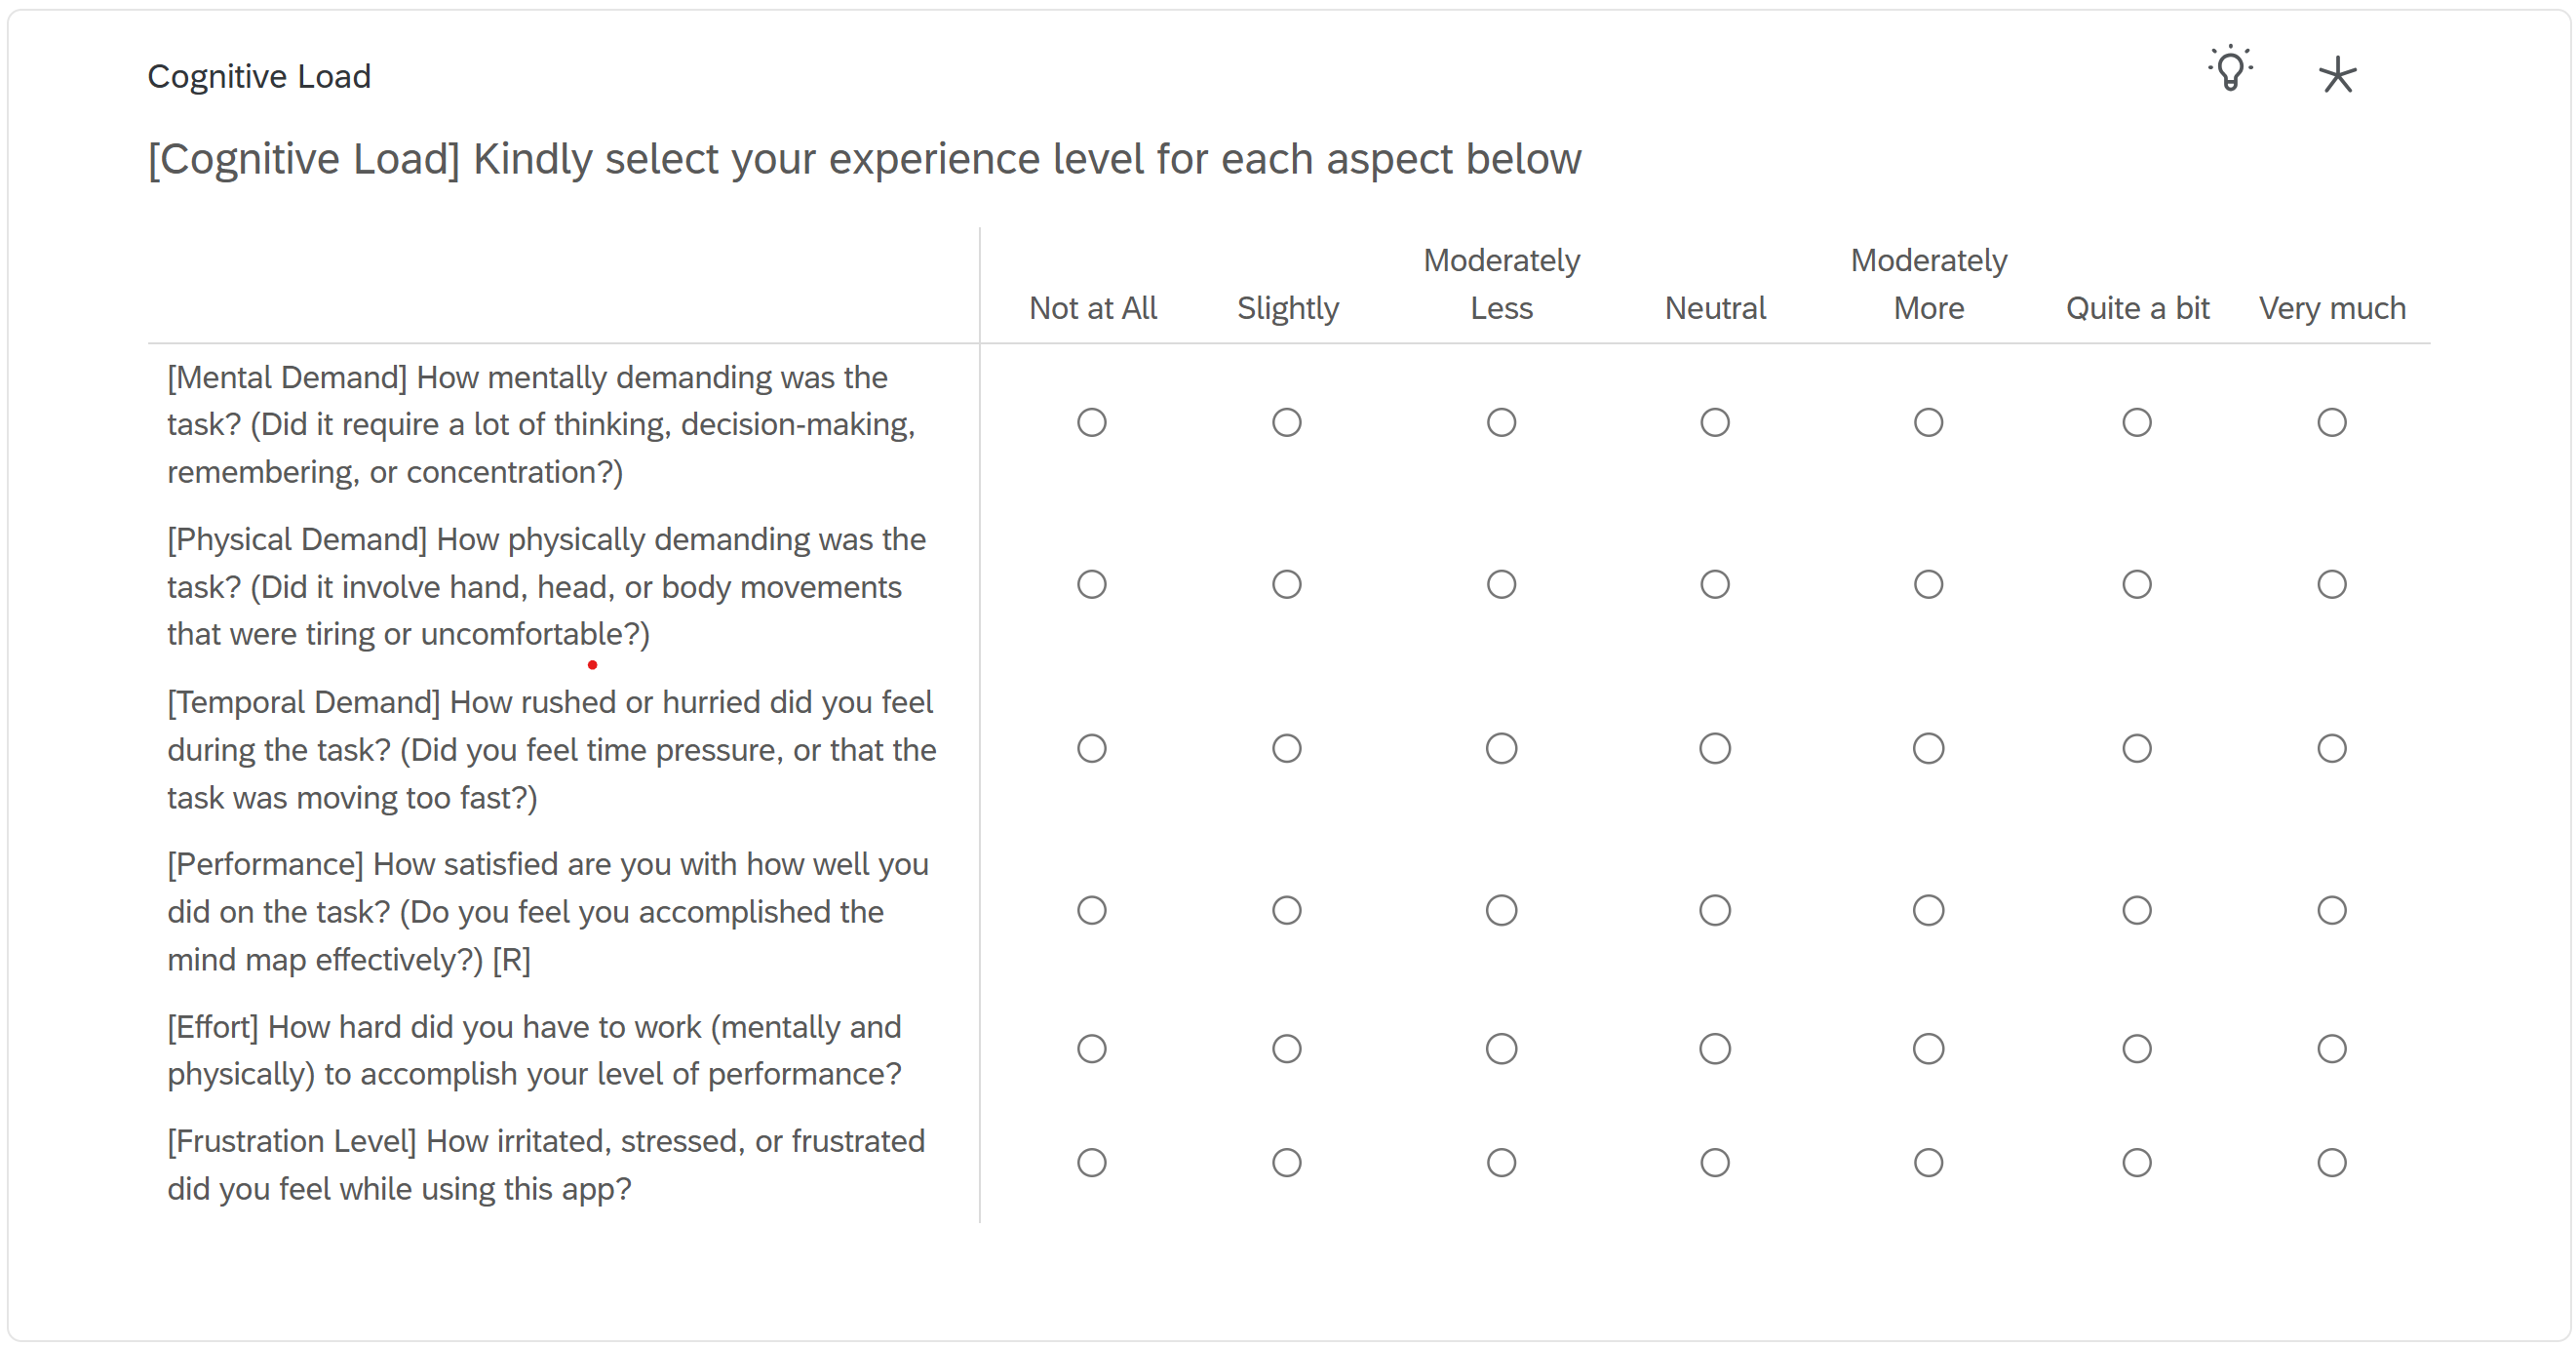
\includegraphics[width=1\linewidth]{fig/Questionnaire/RTLX_1.png}
    \caption{RTLX part of Questionnaire}
    \label{fig:RTLX_1}
\end{figure}


\begin{figure}
    \centering
    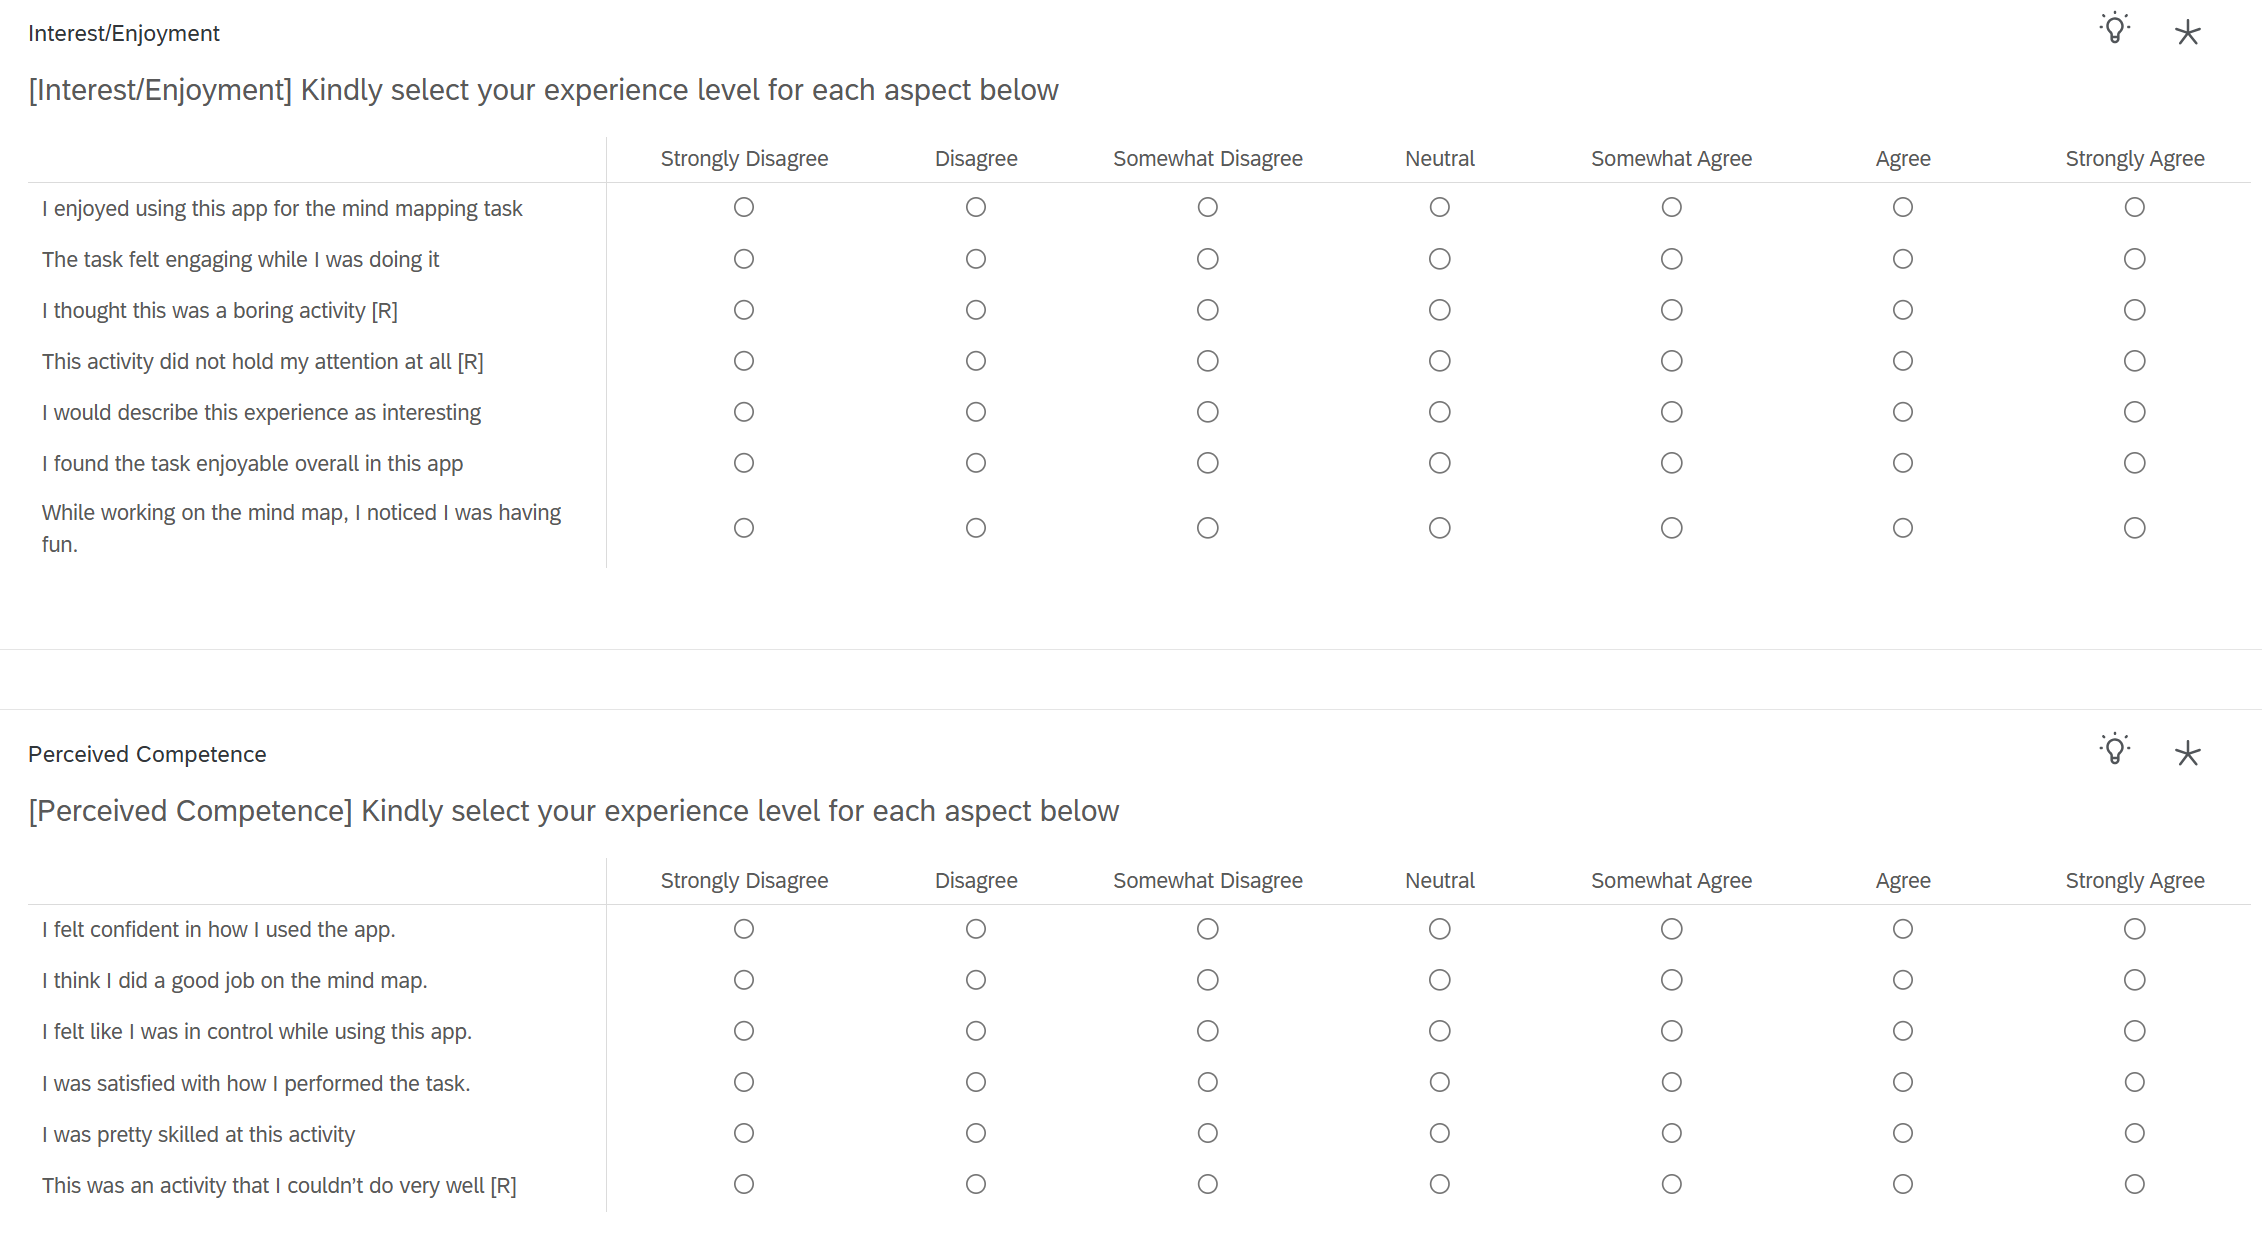
\includegraphics[width=1\linewidth]{fig/Questionnaire/IMI_1_2.png}
    \caption{IMI Part of Questionnaire (Part 1 of 3)}
    \label{fig:IMI_1_2}
\end{figure}

\begin{figure}
    \centering
    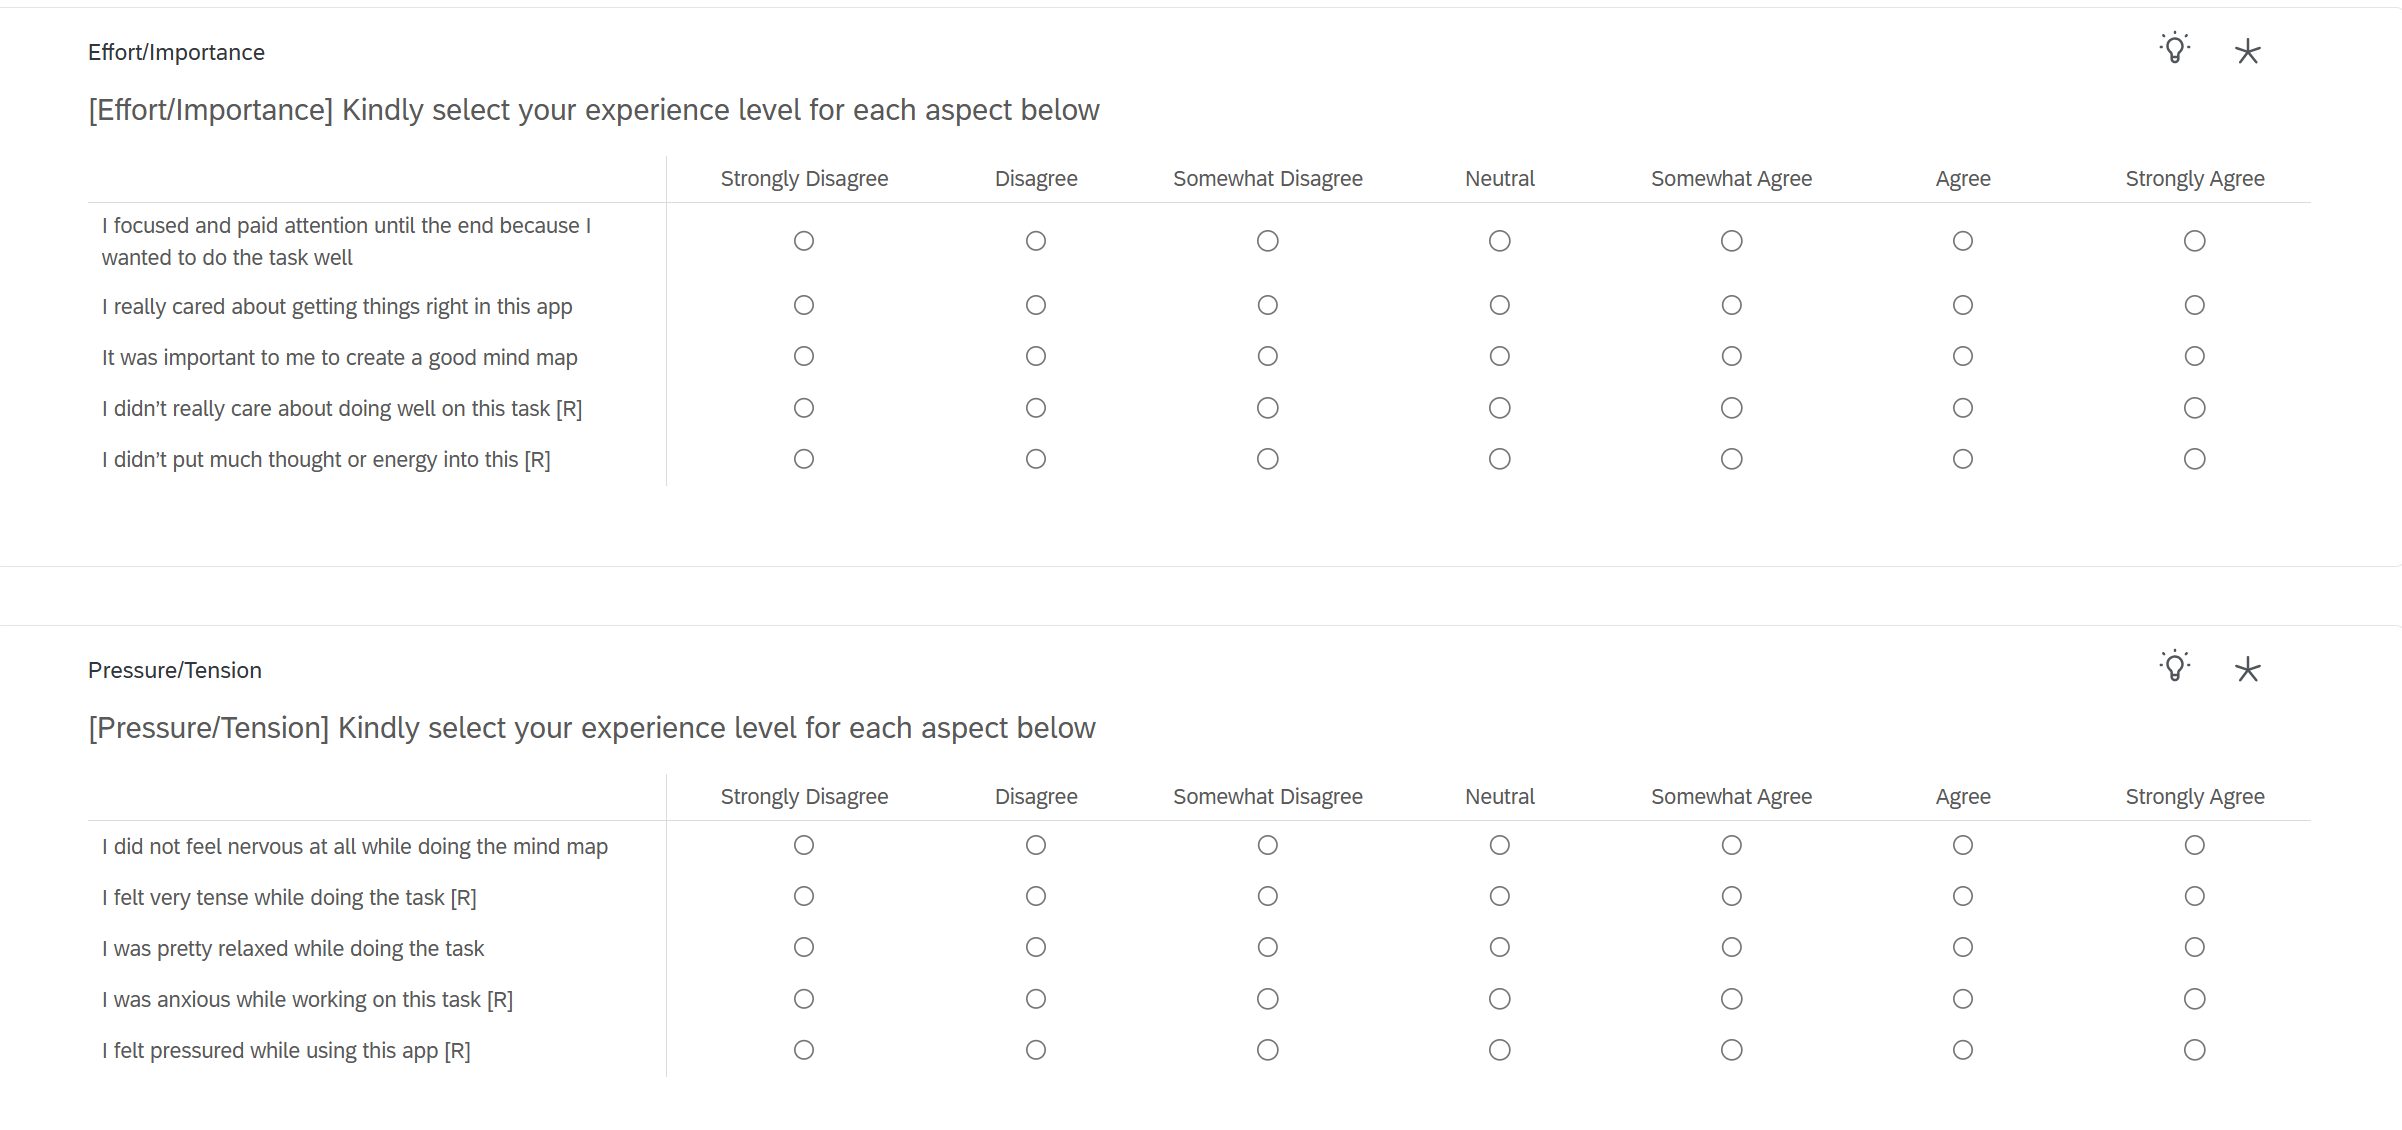
\includegraphics[width=1\linewidth]{fig/Questionnaire/IMI_3_4.png}
    \caption{IMI Part of Questionnaire (Part 2 of 3)}
    \label{fig:IMI_3_4}
\end{figure}

\begin{figure}
    \centering
    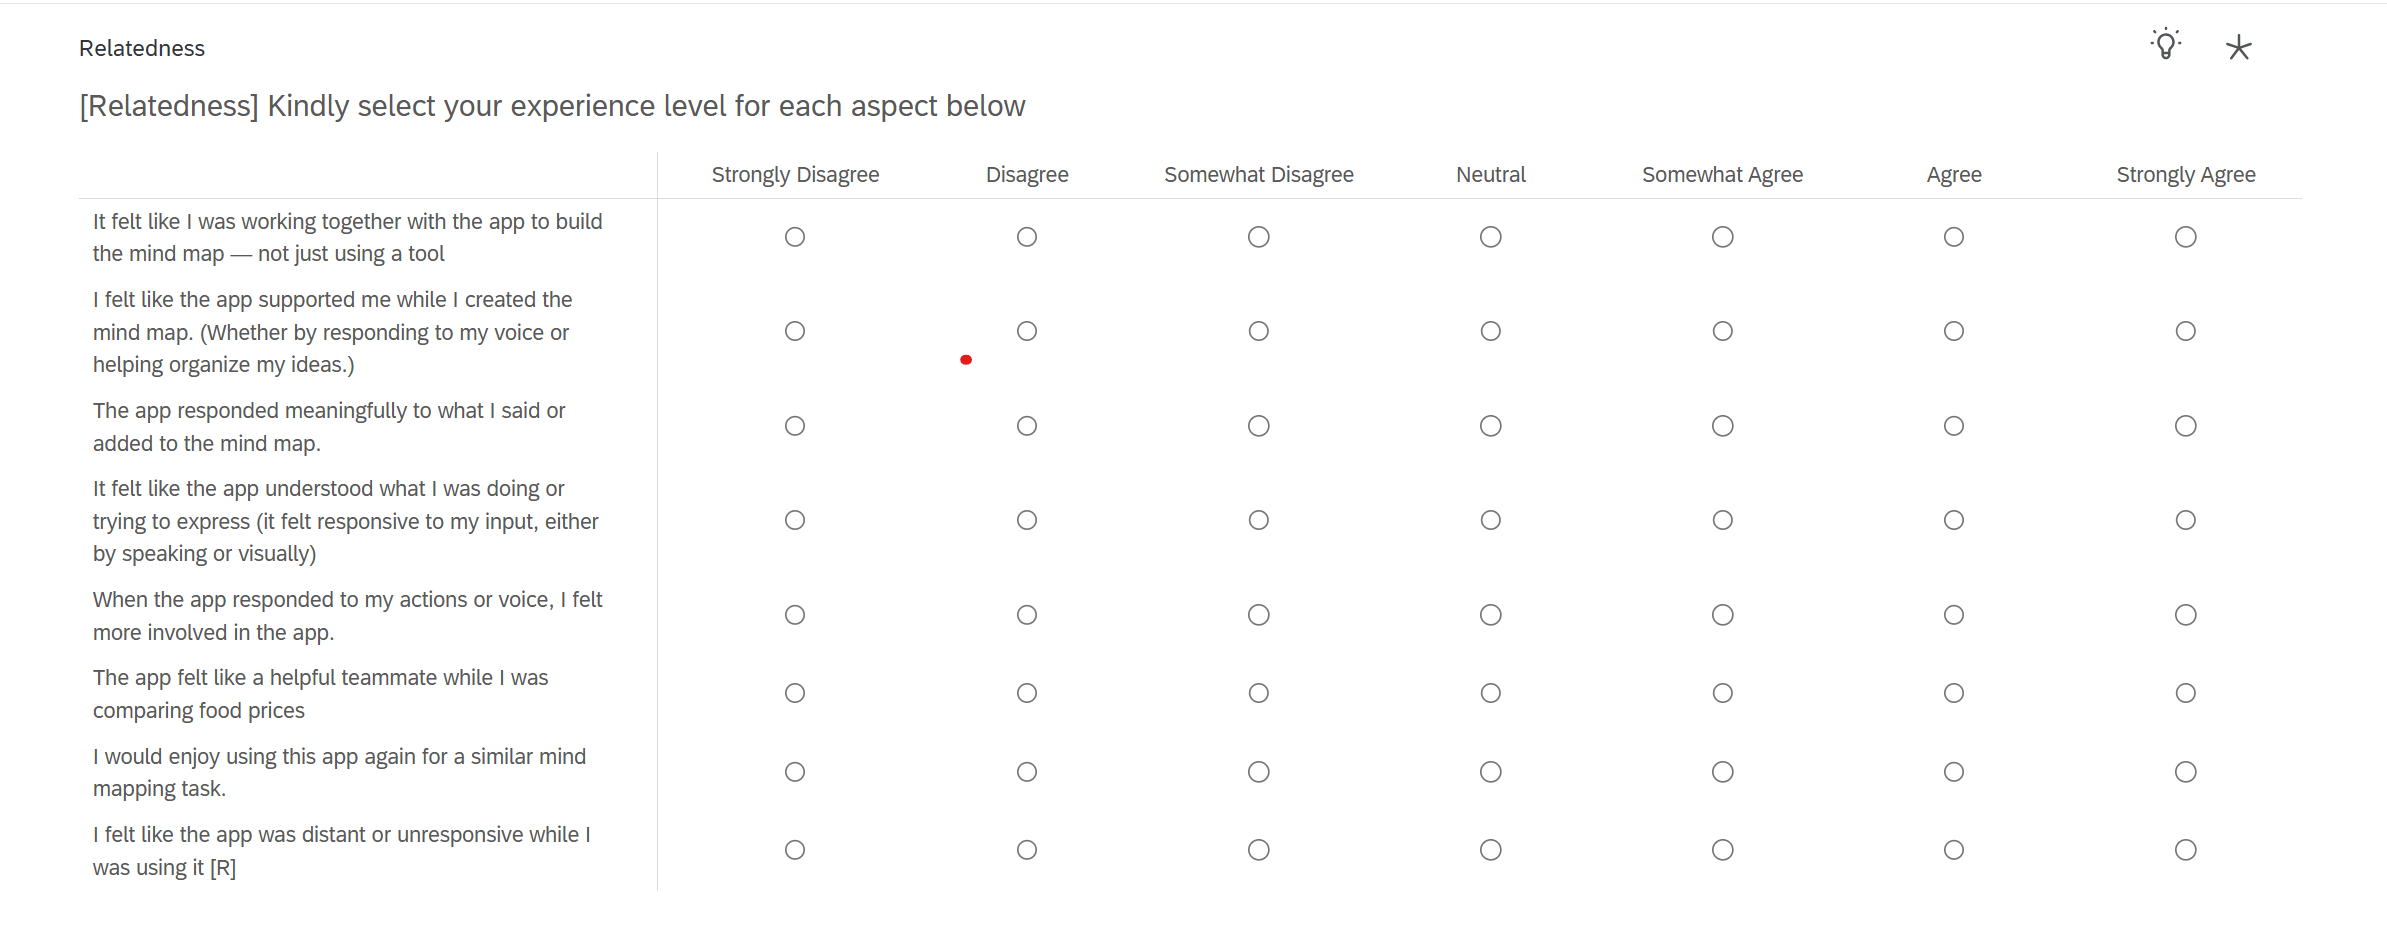
\includegraphics[width=1\linewidth]{fig/Questionnaire/IMI_5.png}
    \caption{IMI Part of Questionnaire (Part 3 of 3)}
    \label{fig:IMI_5}
\end{figure}

\begin{figure}
    \centering
    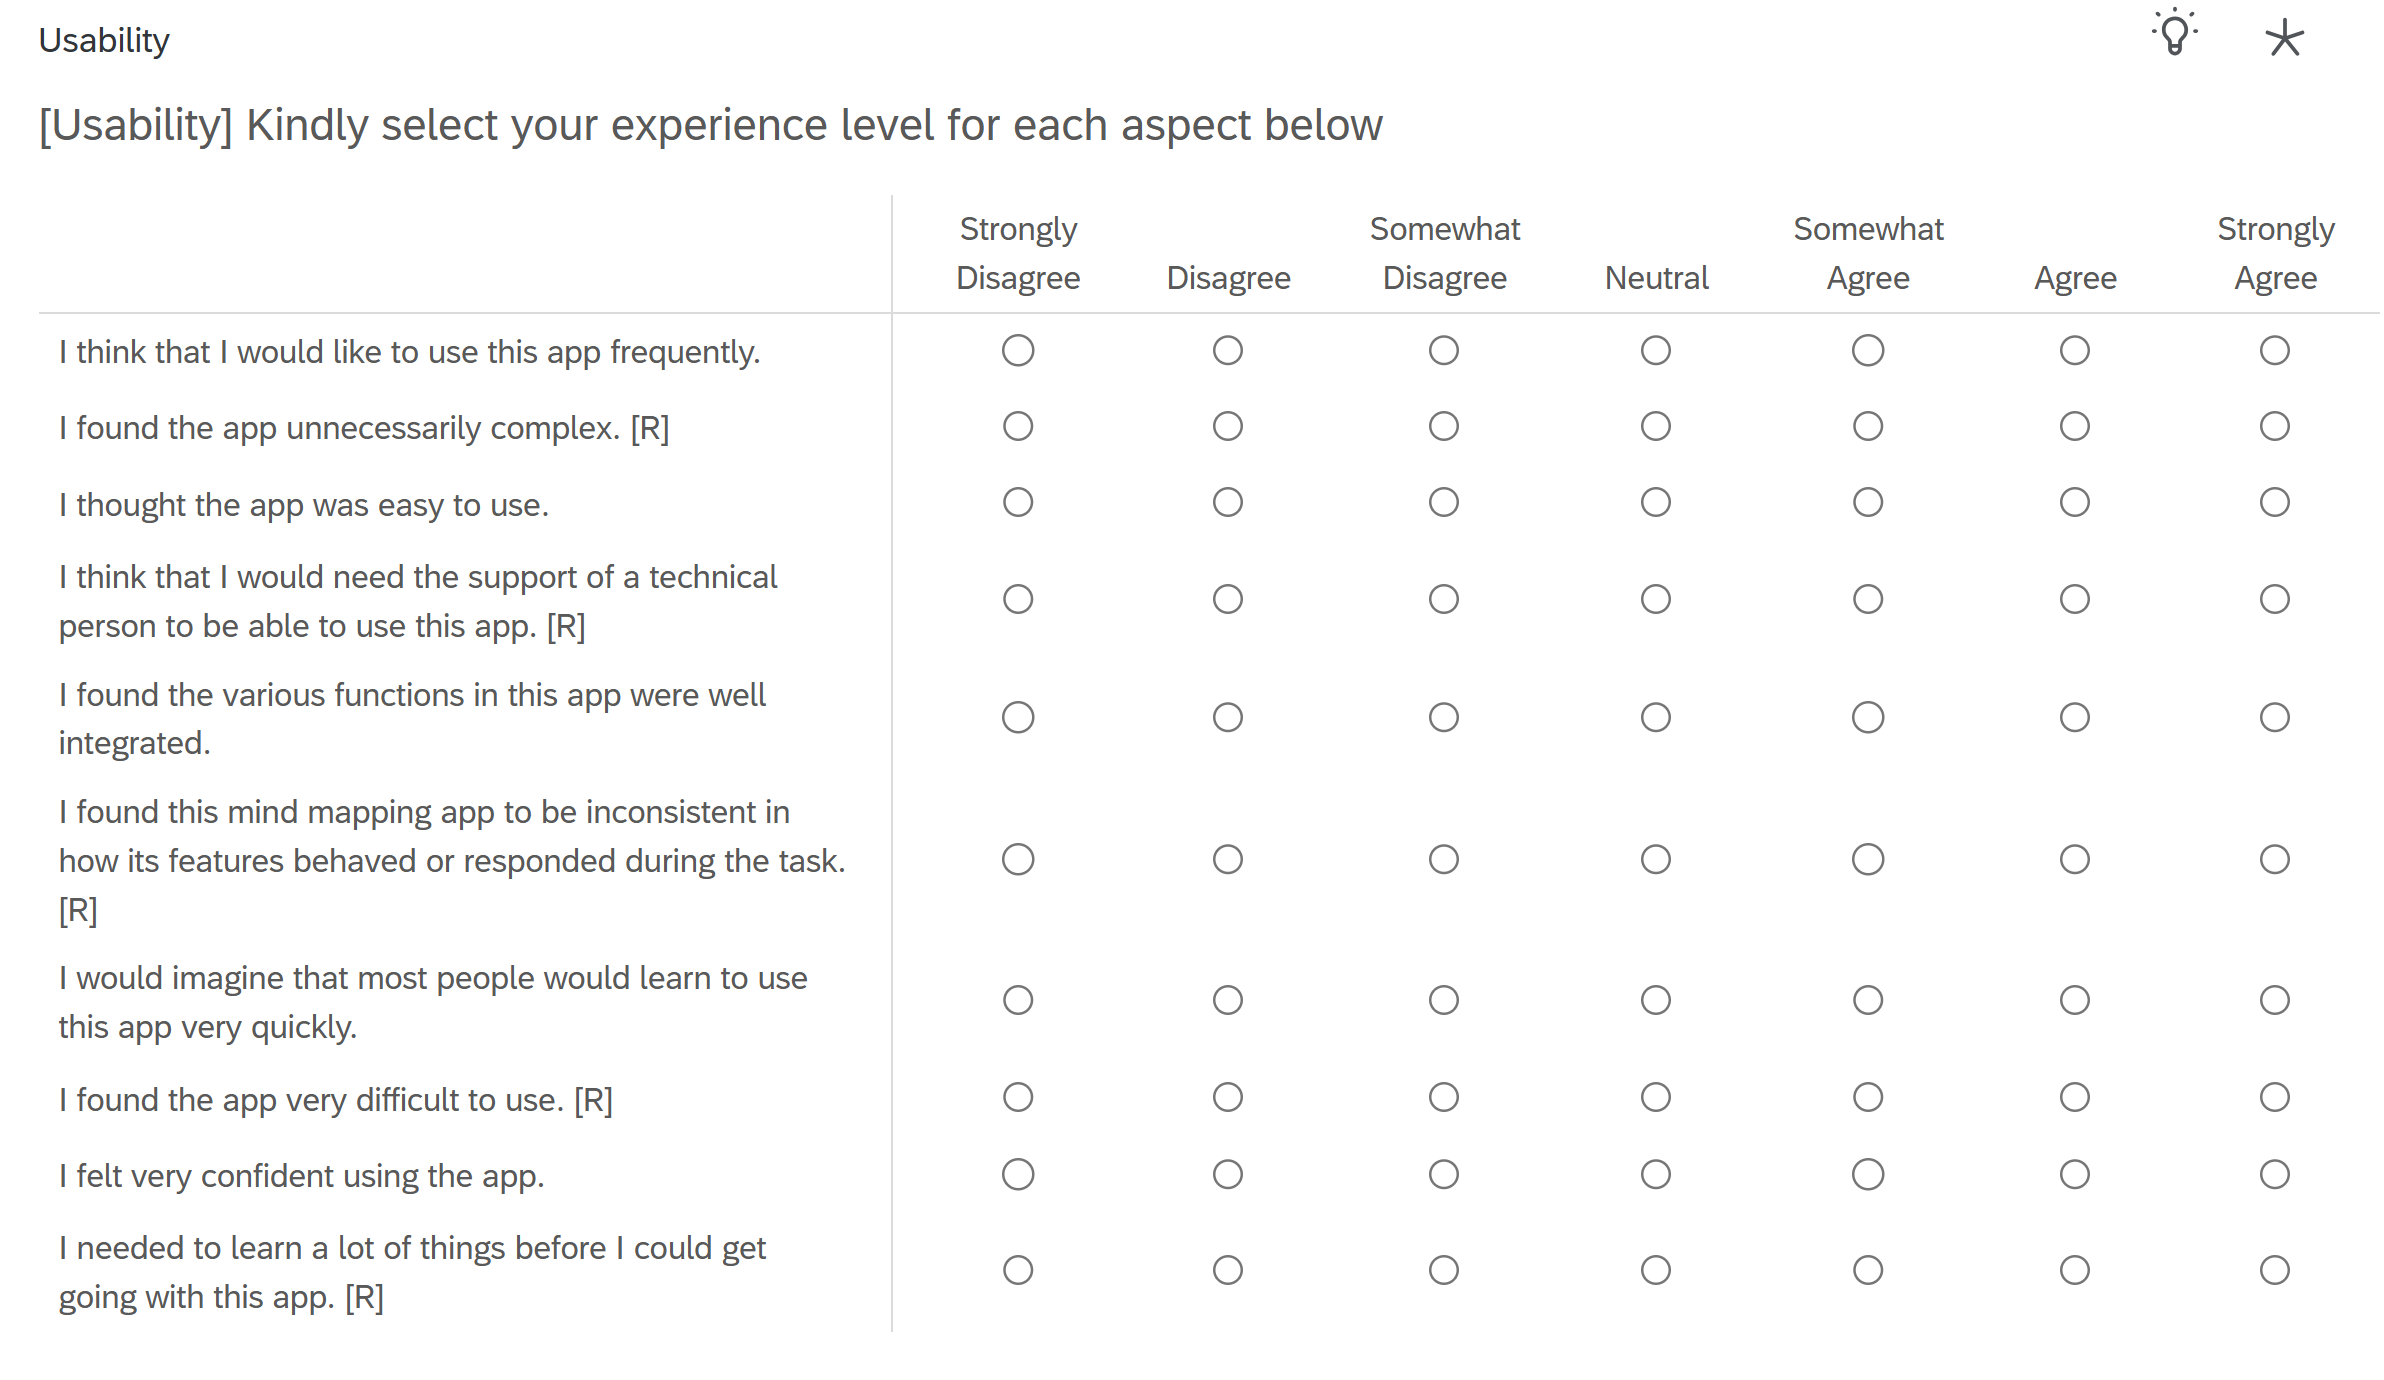
\includegraphics[width=1\linewidth]{fig/Questionnaire/SUS_1.png}
    \caption{SUS part of Questionnaire}
    \label{fig:SUS_1}
\end{figure}


\begin{figure}
    \centering
    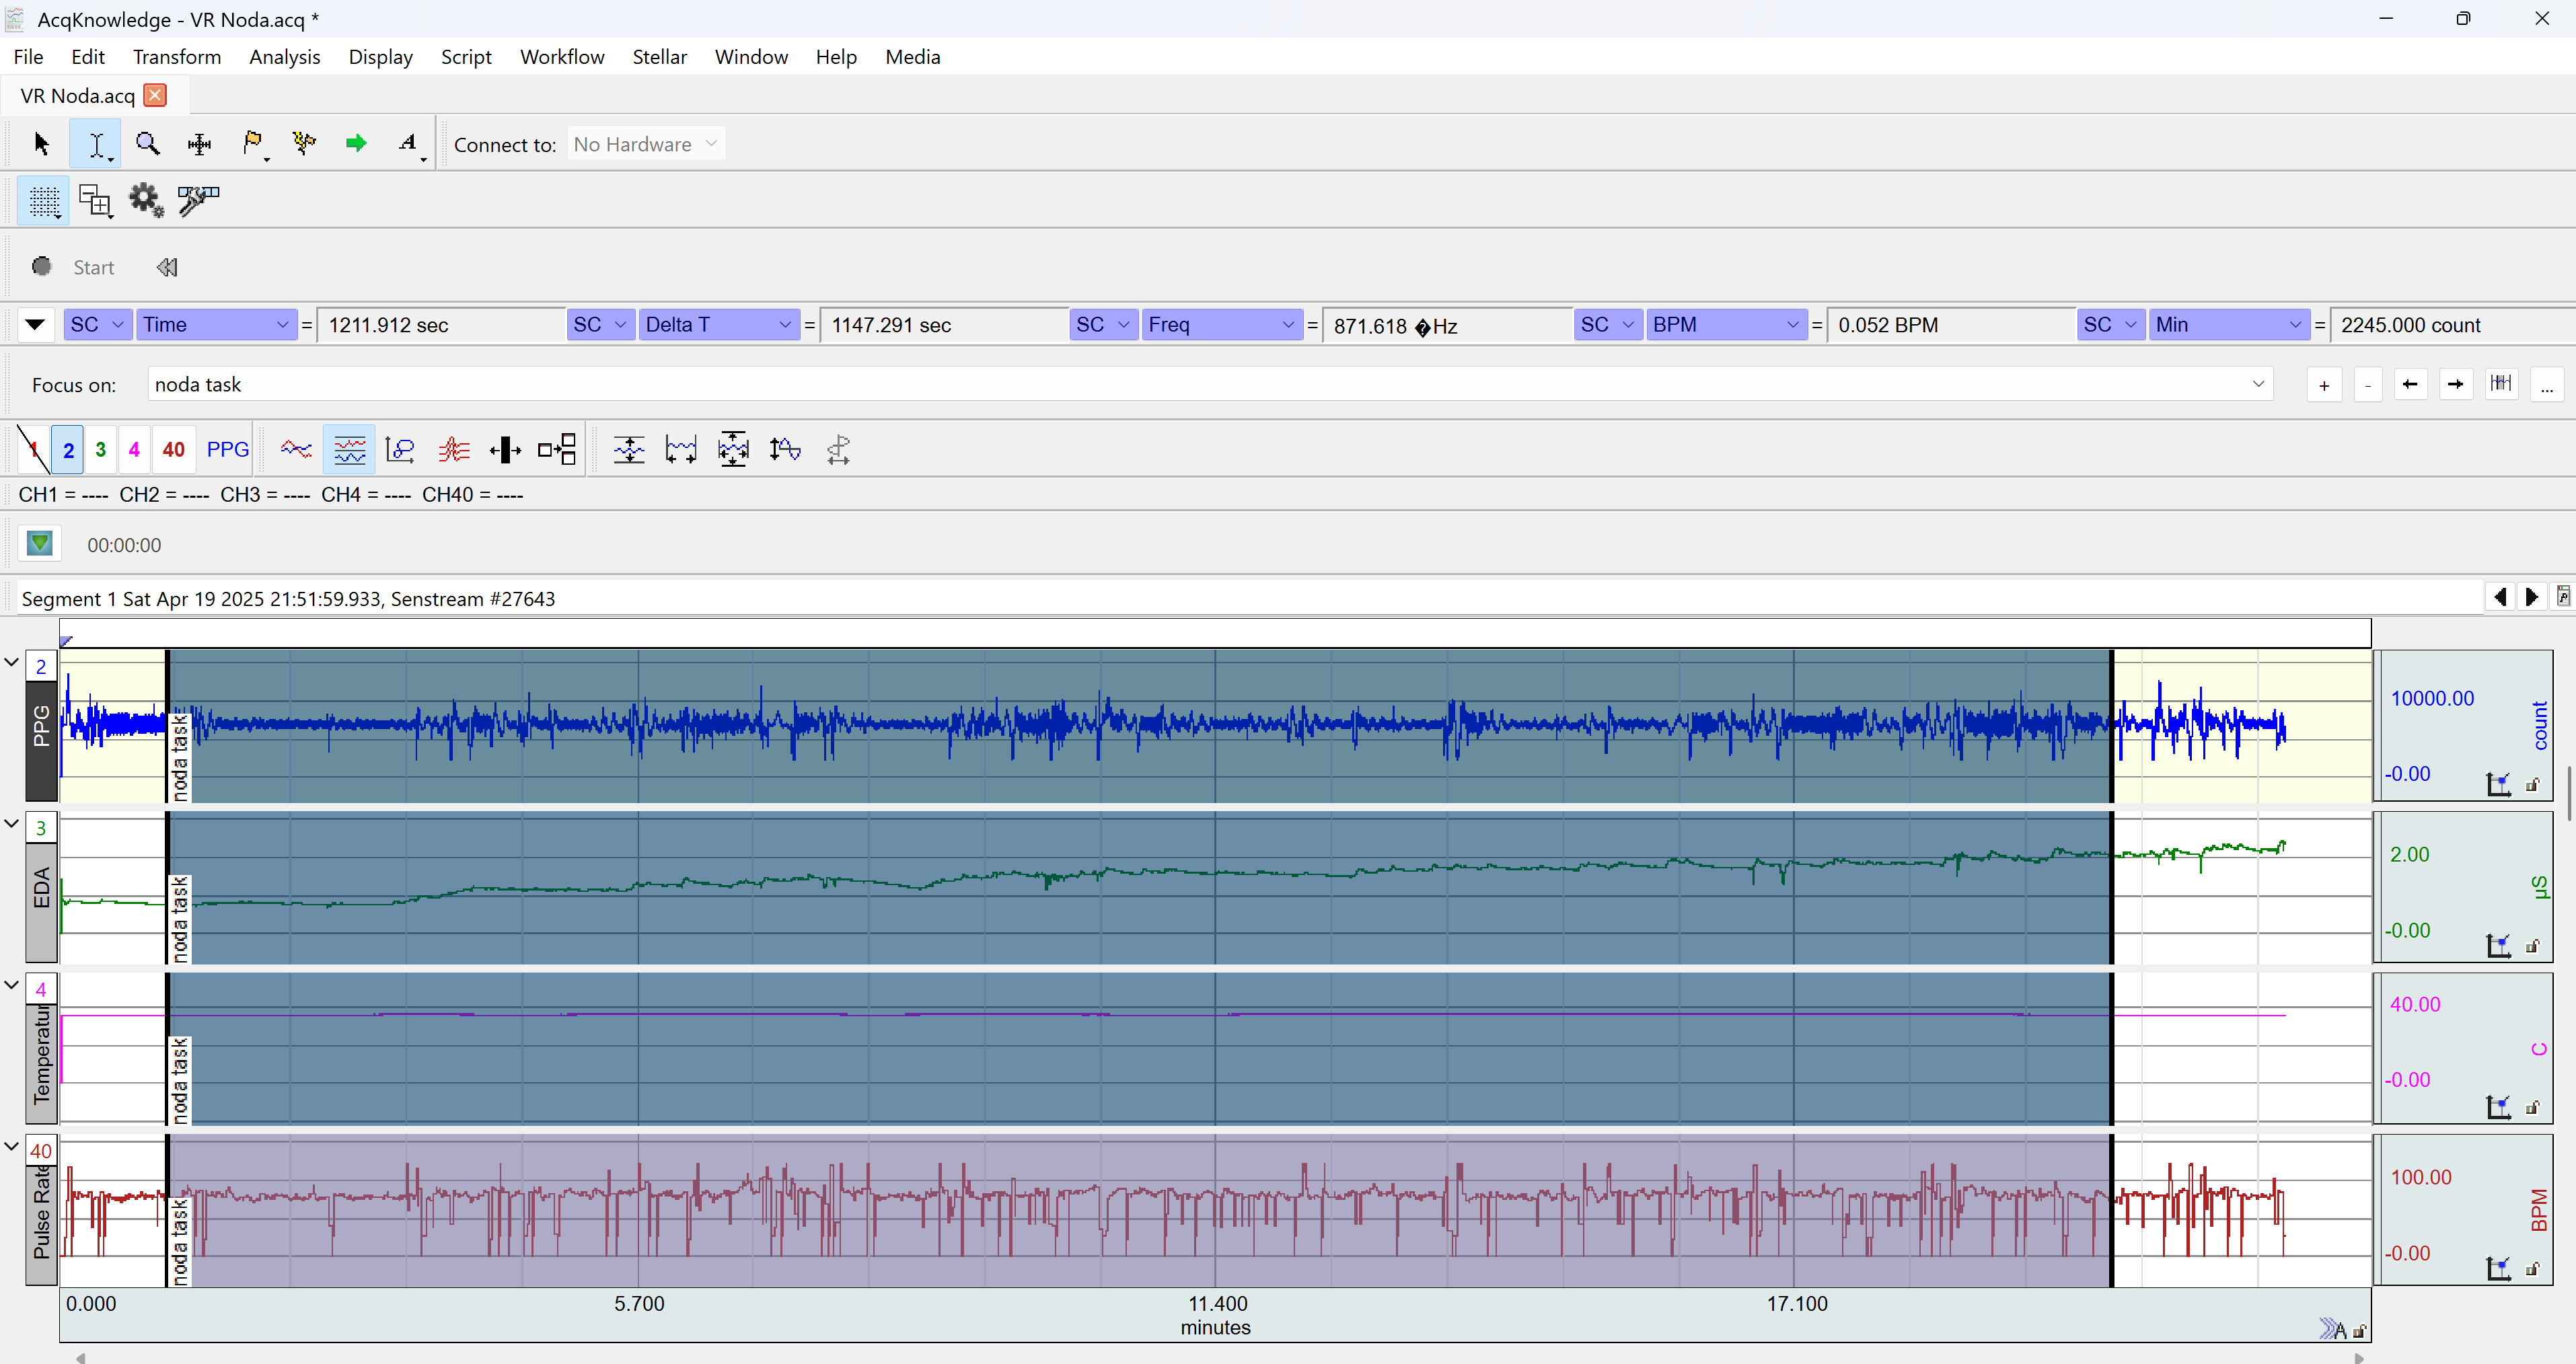
\includegraphics[width=1\linewidth]{fig/physiological/Raw_Noda_FocusArea.png}
    \caption{Raw signals with a selected focus area collected from participant that used Noda}
    \label{fig:Raw_Noda_FocusArea}
\end{figure}


% \end{appendices}



\end{document}


